\chapter{Deploying Liferay DXP}\label{deploying-liferay-dxp}

Liferay DXP is one of the most flexible applications on the market today
with respect to database and application server support. Liferay DXP
supports a wide variety of databases and application servers, freeing
you to use the ones you think are best. Liferay DXP also scales very
well. You can install Liferay DXP on a shared hosting account, on a
multi-node cluster running a commercial application server, or on
anything in between. In fact, Liferay DXP is used successfully in all of
these scenarios every day.

You'll find that because Liferay DXP is extremely flexible in its
deployment options, it is also easy to install. If you already have an
application server, you can use your application server's deployment
tools to install Liferay DXP. If you don't already have an application
server, Liferay provides several application server bundles from which
to choose. These are pre-configured application servers with Liferay DXP
already installed on them. They're easy to install and with a small
amount of configuration can be made into production-ready systems.

Read on to learn how you can prepare to install Liferay DXP.

\section{Preparing for Install}\label{preparing-for-install}

Installing Liferay DXP is easy. But before you begin, you should answer
a few questions.

\begin{itemize}
\tightlist
\item
  Which version of Liferay will you install?
\item
  On which application server will you install Liferay DXP?
\item
  Can you install a Liferay DXP bundle or do you need to install Liferay
  DXP on an existing application server?
\item
  Which database will you use with Liferay DXP?
\item
  How do you plan to store your data?
\item
  Can your network support Liferay DXP?
\end{itemize}

Next, you'll answer these questions and learn the basic steps for
installing Liferay DXP.

\subsection{Obtaining Liferay DXP}\label{obtaining-liferay-dxp}

Anyone can download Liferay DXP from
\href{https://www.liferay.com}{liferay.com}. Click Product →
\emph{Downloads}, and you'll be able to download either the open source
version of Liferay DXP or a trial of the commercial version in several
different formats. These include our convenient bundles as well as
\texttt{.war} files for installing Liferay DXP on your application
server of choice.

Liferay enterprise subscribers can download Liferay DXP from the
\href{https://help.liferay.com/hc}{Help Center}.

So what is a Liferay DXP bundle anyway? A Liferay DXP bundle is an
application server with Liferay DXP pre-installed. Bundles after Liferay
DXP 7.1 GA1 and Liferay Portal CE 7.1 GA1 are released in 7-Zip
(\texttt{.7z}) and gzipped tar (\texttt{.tar.gz}) compressed file
archive formats. Bundles are the easiest way to install Liferay DXP.
Liferay DXP is bundled with a number of application servers; choose the
one that best fits your needs. If you don't currently have an
application server preference, consider starting with the Tomcat bundle.
Tomcat is one of the most lightweight and straightforward bundles to
configure. If you have an open source application server preference,
choose the server you prefer from the available Liferay DXP bundles.
Liferay DXP requires a Java JDK 8 or 11.

\noindent\hrulefill

\textbf{Note:} Please see
\href{https://www.liferay.com/documents/10182/246659966/Liferay+DXP+7.1+Compatibility+Matrix.pdf/c8805b72-c693-1f26-3f2d-731ffc301366}{the
compatibility matrix} for information on supported JDKs, databases, and
environments.

\noindent\hrulefill

Please note that Liferay DXP is not able to provide application server
bundles for proprietary application servers such as WebLogic or
WebSphere, because the licenses for these servers don't allow for
redistribution. Liferay DXP's commercial offering, however, runs just as
well on these application servers as it does on the others. You must
follow our manual installation procedure using a \texttt{.war} file to
install Liferay DXP on proprietary application servers.

Once you have Liferay DXP, you can plan out your installation. First,
prepare your database. Second, install Liferay DXP. Third, configure
your network. Fourth, configure search. You can install Liferay DXP
either by using a bundle or by installing it manually on your existing
application server. Next, we'll go over the steps it takes to install
Liferay DXP.

\subsection{Liferay DXP Installation
Steps}\label{liferay-dxp-installation-steps}

Before you begin installing Liferay DXP, you should review these basic
installation steps:

\begin{enumerate}
\def\labelenumi{\arabic{enumi}.}
\item
  Choose a database server to use with Liferay DXP and create a new
  database. Determine whether you want Liferay DXP to manage your
  database connection or your application server to manage your database
  connection. We recommend that you let Liferay DXP manage your database
  connection. Liferay DXP can connect with several open source or
  enterprise level document repositories.
\item
  Gather mail credentials for sending email notifications to users.
  Determine whether you want Liferay DXP to manage your mail session or
  your application server to manage your mail session. Liferay DXP
  provides a built-in mail session but also supports a JNDI mail
  session. We recommend that you let Liferay DXP manage your mail
  session.
\item
  Install either a Liferay DXP bundle or install Liferay DXP on an
  existing application server (further instructions below).
\item
  Choose IPv4 or IPv6. Determine which address format is best for your
  network (further instructions below).
\item
  Determine how you'll configure Elasticsearch. Liferay DXP's default
  embedded configuration is not supported for production use, so you
  must install Elasticsearch separately, either on the same
  infrastructure or on its own.
\item
  Configure ports (optional). Liferay's application server (e.g., Tomcat
  or Wildfly) uses certain ports for purposes like handling incoming
  HTTP requests, HTTPS requests, or AJP requests, etc. If you start your
  application server in debug mode, there's a port listening for a
  debugger to connect. If desired, you can configure these ports. Please
  refer to your application server's documentation for information on
  its default ports and how to configure them.

  Liferay also provides access to its OSGi framework through a
  configurable port:

  \texttt{module.framework.properties.osgi.console=localhost:11311}

  You can override this default property by copying the line above to
  your \texttt{LIFERAY\_HOME/portal-ext.properties} file and adjusting
  the port number.
\end{enumerate}

We'll go through the steps in order, so first we'll look at the Liferay
DXP database.

\subsection{Step 1: Choose a Database Server and Create a New
Database}\label{step-1-choose-a-database-server-and-create-a-new-database}

The recommended way of setting up your Liferay DXP database is also the
simplest. Liferay DXP takes care of just about everything. You only need
to take two simple steps:

\begin{enumerate}
\def\labelenumi{\arabic{enumi}.}
\tightlist
\item
  Create a blank database encoded with the character set UTF-8. Liferay
  DXP is a multilingual application and needs UTF-8 encoding to display
  all of its supported character sets.
\end{enumerate}

\noindent\hrulefill

\begin{verbatim}
 **Note:** If you plan to migrate from one database vendor to another,
 [configure the database to use the default query result order you expect for entities Liferay DXP lists](/docs/7-0/tutorials/-/knowledge_base/t/sort-order-changed-with-a-different-database).
\end{verbatim}

\noindent\hrulefill

\noindent\hrulefill

\begin{verbatim}
 **Note:** If you use Sybase, configure the database to allow null values by
 default.
\end{verbatim}

\noindent\hrulefill

\begin{enumerate}
\def\labelenumi{\arabic{enumi}.}
\setcounter{enumi}{1}
\tightlist
\item
  Create a database user for accessing this database. Grant this
  database user all rights, including the rights to create and drop
  tables, to the blank Liferay DXP database.
\end{enumerate}

\noindent\hrulefill

\begin{verbatim}
 **Important:** Liferay requires reading from and writing to the database.
 The Liferay database user must therefore have permissions to read and
 write data.
\end{verbatim}

\noindent\hrulefill

Liferay DXP uses this database user's credentials to connect to the
Liferay DXP database either directly or through its application server.
During its initial startup, Liferay DXP creates the tables it needs in
the database you just created. It does this automatically, complete with
indexes.

This is the recommended way to set up Liferay DXP. It enables Liferay
DXP to maintain its database automatically during upgrades or when
various Liferay DXP plugins that create database tables of their own are
installed. This method is by far the best way to set up your Liferay DXP
database.

\noindent\hrulefill

\textbf{Warning:} If you're using an Oracle database, use the
\texttt{ojdbc8.jar} driver library with at least Oracle 12.2.0.1.0 JDBC
4.2 versioning because
\href{https://issues.liferay.com/browse/LPS-79229}{data truncation
issues} have been detected reading data from CLOB columns.

\noindent\hrulefill

If you choose to set up Liferay DXP's database with the recommended
permissions described in this section, you can skip to the next section.

\noindent\hrulefill

\textbf{Warning:} The instructions below are not ideal for Liferay DXP
installations. This procedure is documented here so that enterprises
with more restrictive standards can install Liferay DXP with stricter
(but sub-optimal) database settings. If it's at all possible, we
recommend that you use the method described in the previous section
instead of the procedure outlined below.

\noindent\hrulefill

Even though Liferay DXP can create its database automatically, some
enterprises prefer \emph{not} to allow the database user configured in
an application server to have the database permissions necessary for
Liferay DXP and its plugins to maintain their tables. For these
organizations, Select, Insert, Update and Delete are the only allowed
permissions. Thus, in this section we explain how to set up the database
manually. If your organization \emph{is} willing to grant the Liferay
DXP database user the permissions to create and drop tables in the
database--and this is the recommended configuration--then simply use the
recommended configuration described in the previous section.

\begin{enumerate}
\def\labelenumi{\arabic{enumi}.}
\item
  Create a new, blank, database for Liferay DXP.
\item
  Grant full rights to do anything to the Liferay DXP database to the
  Liferay DXP database user.
\item
  Install Liferay DXP and start it so that it automatically populates
  its database.
\item
  Once the database has been populated with the Liferay DXP tables,
  remove the permissions for creating and dropping tables from the
  Liferay DXP database user.
\end{enumerate}

There are some caveats to running Liferay DXP like this. Many Liferay
DXP plugins create new tables when they're deployed. Additionally,
Liferay DXP has an automatic database upgrade function that runs when
Liferay DXP is upgraded. If the Liferay DXP database user doesn't have
enough rights to create/modify/drop tables in the database, you must
grant those rights to the ID before you deploy one of these plugins or
start upgrading Liferay DXP. Once the tables are created or the upgrade
is complete, you can remove those rights until the next deploy or
upgrade. Additionally, your own developers might create plugins that
need to create their own tables. These are just like Liferay DXP's
plugins that do the same thing, and they cannot be installed if Liferay
DXP can't create database tables. If you wish to install these plugins,
you will need to grant rights to create tables in the database each time
before you attempt to install them.

Liferay DXP offers several configurations to store Documents and Media
files by setting the \texttt{dl.store.impl=} property. Available options
are Simple File System Store, Advanced File System Store, CMIS Store,
DBStore, JCRStore, and Amazon S3Store. In addition, Liferay DXP can be
connected to various open source and enterprise-level document
repositories. All of the repositories are connected to Liferay DXP
through hooks available on Liferay Marketplace (see below).

Once you have your database and document repository ready, you can
install Liferay DXP on your server.

\subsection{Step 2: Gather Your Mail
Credentials}\label{step-2-gather-your-mail-credentials}

Liferay DXP uses a mail server to send email notifications. As part of
the install, therefore, you will need to have credentials that Liferay
DXP can use to connect to your mail server. Specifically, you'll need to
have the following information:

\begin{itemize}
\tightlist
\item
  Incoming POP Server and port
\item
  POP User Name
\item
  POP Password
\item
  Outgoing SMTP Server and port
\item
  SMTP User Name
\item
  SMTP Password
\item
  A list of JavaMail properties that would override a default
  configuration
\end{itemize}

Once you've gathered this information, you're ready to move on to the
next step.

\subsection{Step 3: Install}\label{step-3-install}

The next step is to install Liferay DXP. You can do this in one of two
ways: by
\href{/docs/7-1/deploy/-/knowledge_base/d/installing-liferay}{installing
Liferay DXP bundled with an application server}, or by
\href{/docs/7-1/deploy/-/knowledge_base/d/installing-liferay-manually}{installing
Liferay DXP manually on an existing application server}. Each Liferay
DXP installation's
\href{/docs/7-1/deploy/-/knowledge_base/d/installing-liferay\#liferay-home}{Liferay
Home contains several folders}.

By far the easiest way to get Liferay DXP installed is to use a bundle.
Though bundles are pre-packaged for demo purposes, it is very easy to
turn them into full, production-ready Liferay DXP instances.

\subsection{Step 4: Network
Configuration}\label{step-4-network-configuration}

Liferay DXP supports both IPv4 and IPv6 address formats. You must
\href{/docs/7-0/deploy/-/knowledge_base/d/choosing-ipv4-or-ipv6}{choose
between IPv4 or IPv6}. By default, Liferay DXP uses IPv4 addresses. If
you are using IPv6, you will have to configure Liferay DXP. There are
two simple steps.

\begin{enumerate}
\def\labelenumi{\arabic{enumi}.}
\item
  In the application server's environment settings, set
  \texttt{-Djava.net.preferIPv4Stack=false}.
\item
  Create a \texttt{portal-ext.properties} file in your portal's
  \href{/docs/7-1/deploy/-/knowledge_base/d/installing-liferay\#liferay-home}{Liferay
  Home folder} (if one does not already exist) and set the
  \texttt{tunnel.servlet.hosts.allowed} property to the target hosts you
  want to allow (e.g., \emph{0:0:0:0:0:0:0:1}).
\end{enumerate}

\subsection{Step 5: Configure
Elasticsearch}\label{step-5-configure-elasticsearch}

Liferay DXP by default ships with an embedded version of Elasticsearch.
While this configuration works well for demo purposes, it is not
supported in a production installation. After you install Liferay DXP,
you'll need to configure it to connect to a standalone Elasticsearch
server or cluster. Depending on the size of your installation, this
standalone instance of Elasticsearch can reside either on the same
machine you have Liferay DXP on or a different machine. For performance
purposes, it is better to
\href{/docs/7-1/deploy/-/knowledge_base/d/installing-elasticsearch}{install
Elasticsearch on a separate machine}.

\subsection{Step 6: Liferay Marketplace and Portal
Security}\label{step-6-liferay-marketplace-and-portal-security}

The Liferay Marketplace is an integral part of the Liferay DXP
experience. The Marketplace plugin is required to be installed on
Liferay DXP. The Marketplace plugin enables a host of features that
extend beyond just access to the online Liferay Marketplace. Some of the
key features the Marketplace plugin enables are

\begin{itemize}
\tightlist
\item
  Liferay Marketplace: direct access to our online Marketplace
\item
  App Manager: ability to install, uninstall, and update apps
\item
  Bundled Apps: easily manage apps that may come bundled with your
  Liferay DXP
\item
  Developer Apps: ability to manage apps that you're developing
\item
  License Manager: streamlined license management for your Liferay DXP
  and apps
\end{itemize}

The portal installation process deploys and registers the Marketplace
plugin automatically. If you're installing Liferay DXP in an environment
that would prevent this from happening, you'll have to perform one of
several workarounds.

Now that you know where you're headed, you can install Liferay DXP. If
you have decided to install Liferay DXP using a bundle, continue with
the next section. If you're installing Liferay DXP manually, skip to the
section for your application server of choice. Once you have Liferay DXP
installed manually or via a bundle, you can move on to
\href{/docs/7-1/deploy/-/knowledge_base/d/installing-liferay\#\#using-liferays-setup-wizard}{using
Liferay DXP's Setup Wizard},
\href{/docs/7-1/deploy/-/knowledge_base/d/installing-liferay\#configuring-mail}{configuring
mail}, and
\href{/docs/7-1/deploy/-/knowledge_base/d/installing-elasticsearch}{installing
Elasticsearch}.

\section{Installing Liferay DXP}\label{installing-liferay-dxp}

Now that you've performed the steps needed to
\href{/docs/7-1/deploy/-/knowledge_base/d/preparing-for-install}{prepare
for your installation}, you're ready to install Liferay DXP! Since
bundles are the easiest way to complete an installation, all the
installation steps below assume you're installing a Liferay DXP bundle.
If you plan to install Liferay DXP manually, please refer to the article
for your app server of choice, and then come back here to complete the
configuration steps.

Now you're ready. You've created a blank database for Liferay DXP and
have gathered the credentials you need for your mail server. The next
step is to install Liferay DXP.

\subsection{Liferay Home}\label{liferay-home}

Liferay DXP bundles contain the same folder structure regardless of
application server. The top-level folder is named for the Liferay DXP
release. This folder is called \emph{Liferay Home}. This folder is
usually the application server's parent folder. This is why Liferay DXP
bundles place the application server inside the bundle's root folder. On
a manual installation, the location of this folder varies by application
server. In a bundle, it's part of the bundle. If you're doing a manual
installation, please refer to the article covering that app server for
its location.

Liferay Home has folders for various purposes:

\begin{itemize}
\tightlist
\item
  \textbf{\hyperref[liferay-home]{Liferay Home}}

  \begin{itemize}
  \item
    \textbf{{[}Application Server{]}}: The name of this folder varies
    depending on the bundle you're using. This folder contains the
    application server in which Liferay DXP has been installed.
  \item
    \texttt{data}: Stores an embedded HSQL database, Liferay DXP's file
    repository, and Liferay DXP's search indexes. Liferay DXP is
    initially configured to use the embedded HSQL database but the HSQL
    database is primarily intended for demonstration and trial purposes.
    \href{https://docs.liferay.com/dxp/portal/7.1-latest/propertiesdoc/portal.properties.html\#JDBC}{Portal
    property \texttt{jdbc.default.url}} sets the Hypersonic embedded
    HSQL database location.
  \item
    \texttt{deploy}: To auto-deploy Liferay DXP plugins, copy them to
    this folder. Legacy style \texttt{.war} files, 7.0 style
    \texttt{.jar} files, and \texttt{.lpkg} files from Liferay
    Marketplace are supported.
    \href{https://docs.liferay.com/dxp/portal/7.1-latest/propertiesdoc/portal.properties.html\#Auto\%20Deploy}{Portal
    property \texttt{auto.deploy.deploy.dir}} sets the auto-deploy
    location.
  \item
    \texttt{license}: Liferay DXP's copyright and version files are
    here.
  \item
    \texttt{logs}: This folder contains Liferay DXP's log files. The
    information in Liferay DXP's log files can be quite valuable for
    system administrators, especially when trying to diagnose a problem.
    \texttt{portal-impl.jar}'s
    \texttt{portal-impl/src/META-INF/portal-log4j.xml} file sets the
    location for the log files. To override the log file location, you
    must
    \href{/docs/7-0/tutorials/-/knowledge_base/t/advanced-customization-with-ext-plugins\#using-advanced-configuration-files}{use
    an \texttt{ext-impl/src/META-INF/portal-log4j-ext.xml} file in an
    Ext plugin}.
  \item
    \texttt{osgi}: All the JAR files and a few configuration files for
    Liferay DXP's OSGi runtime belong in this folder.
    \href{https://docs.liferay.com/dxp/portal/7.1-latest/propertiesdoc/portal.properties.html\#Module\%20Framework}{Portal
    property \texttt{module.framework.base.dir}} sets the OSGi folder
    location. Here are its subfolders:

    \begin{itemize}
    \tightlist
    \item
      \texttt{configs}: Component configuration files go here
    \item
      \texttt{core}: Liferay DXP's core modules
    \item
      \texttt{marketplace}: Marketplace applications and application
      suites
    \item
      \texttt{modules}: Modules you've deployed
    \item
      \texttt{portal}: Liferay DXP's non-core modules
    \item
      \texttt{state}: Contains OSGi internal state files for such things
      as OSGi bundle installation, bundle storage, and more
    \item
      \texttt{target-platform}: Target platform index
    \item
      \texttt{test}: Modules that support test integration
    \item
      \texttt{war}: WAR plugins you've deployed
    \end{itemize}
  \item
    \texttt{patching-tool}: (Liferay DXP only) This folder contains
    patches for Liferay DXP and files for installing the patches.
  \item
    \texttt{tools}: For Liferay DXP upgrade and target platform indexer.
  \item
    \texttt{work}: Module Jasper work files.
  \end{itemize}
\end{itemize}

If Liferay DXP is unable to create the resources it needs in the Liferay
Home folder or if it finds itself running on certain application
servers, it creates a folder called \texttt{liferay} in the home folder
of the operating system user that is running Liferay DXP. In this case,
the \texttt{liferay} folder becomes Liferay Home. For example, if the
operating system user's name is jbloggs, the Liferay Home folder is
\texttt{/home/jbloggs/liferay} or
\texttt{C:\textbackslash{}Users\textbackslash{}jbloggs\textbackslash{}liferay}.

\subsection{Extracting a Liferay
Bundle}\label{extracting-a-liferay-bundle}

Getting a Liferay DXP bundle up and running involves uncompressing the
archive, possibly copying a JDBC driver, and then starting the
application server. Let's use the Liferay DXP Tomcat bundle as an
example.

\begin{enumerate}
\def\labelenumi{\arabic{enumi}.}
\tightlist
\item
  Extract your Liferay DXP bundle.
\item
  If you're using a supported open source database or if you're setting
  up Liferay DXP for demo purposes, you can skip this step. Otherwise,
  copy your database's JDBC driver \texttt{.jar} file to
  \texttt{{[}Tomcat{]}/lib/ext}.
\end{enumerate}

That's it! You've extracted Liferay DXP, and it's ready for use. This is
much easier than doing a manual installation on an app server. If,
however, that's what you need to do, please at this point click the link
on the left and go through the installation procedure for your app
server of choice. When you're finished with the installation (and before
you've started Liferay DXP for the first time), come back to this spot,
because you must hook it up to your database.

\noindent\hrulefill

\textbf{Important:} On JDK 11, the setting
\texttt{-Djava.locale.providers=JRE,COMPAT,CLDR} is required to display
four-digit years. Since JDK 9, the Unicode Common Locale Data Repository
(CLDR) is the default locales provider. CLDR does not provide years in a
four-digit format (see
\href{https://issues.liferay.com/browse/LPS-87191}{LPS-87191}). This
setting works around the issue by using JDK 8's default locales
provider. Please see
\href{/docs/7-1/deploy/-/knowledge_base/d/installing-product-on-tomcat\#configuring-tomcat}{Installing
Liferay DXP on Tomcat} for more information.

\noindent\hrulefill

\subsection{Connecting to Your
Database}\label{connecting-to-your-database}

You can connect to your database with JNDI on your app server or the
data source shipped with Liferay DXP (recommended). Refer to the article
on your app server for instructions on using JNDI. For the internal data
source, you can configure it by specifying the configuration in a
\texttt{portal-ext.properties} file or the
\href{/docs/7-1/deploy/-/knowledge_base/d/installing-liferay\#using-the-setup-wizard}{Setup
Wizard}:

\begin{enumerate}
\def\labelenumi{\arabic{enumi}.}
\item
  Create a \texttt{portal-ext.properties} file in your Liferay Home
  folder.
\item
  Copy a relevant example data source configuration from one of the
  \href{/docs/7-1/deploy/-/knowledge_base/d/database-templates}{data
  source configuration templates} or
  \href{https://docs.liferay.com/dxp/portal/7.1-latest/propertiesdoc/portal.properties.html\#JDBC}{portal
  properties reference's JDBC section} and paste it into the
  \texttt{portal-ext.properties} file.
\item
  Customize the configuration with the proper host name and user and
  password credentials for your database, and save the file.
\end{enumerate}

You're ready to start Liferay DXP.

\subsection{Running for the First
Time}\label{running-for-the-first-time}

Next, start your app server, or start the Liferay DXP app in your app
server. Liferay DXP writes log files to folder
\texttt{{[}Liferay\ Home{]}/logs}.

The first time Liferay DXP starts, it creates all of its database
tables. Once it has successfully started, it automatically launches a
web browser that displays the Basic Configuration page. If for some
reason your browser doesn't load the Basic Configuration page, launch it
and navigate to your app server's address and port (for example,
http://localhost:8080).

\subsection{Using the Setup Wizard}\label{using-the-setup-wizard}

The Setup Wizard runs when you start Liferay DXP for the first time. The
title of the setup wizard page is Basic Configuration. This page
provides a convenient way to make an initial configuration.

There are two sections of the wizard: the portal and the administrator.
For the portal, you need to supply the following information:

\textbf{Portal Name:} the name of the portal you're powering with
Liferay DXP.

\textbf{Default Language:} choose the default locale of your portal.

\textbf{Time Zone:} select your Liferay DXP instance's default time
zone.

For the administrator, you need to supply the following information:

\textbf{First Name:} the first name of the default administrator user

\textbf{Last Name:} the last name of the default administrator user

\textbf{Email:} the email address of the default administrator user

\noindent\hrulefill

\textbf{Note:} the administrator user's email domain is used as the
Liferay DXP instance's default domain (i.e., the
\href{https://docs.liferay.com/dxp/portal/7.1-latest/propertiesdoc/portal.properties.html\#Company}{\texttt{company.default.web.id}}
portal property).

\noindent\hrulefill

\begin{figure}
\centering
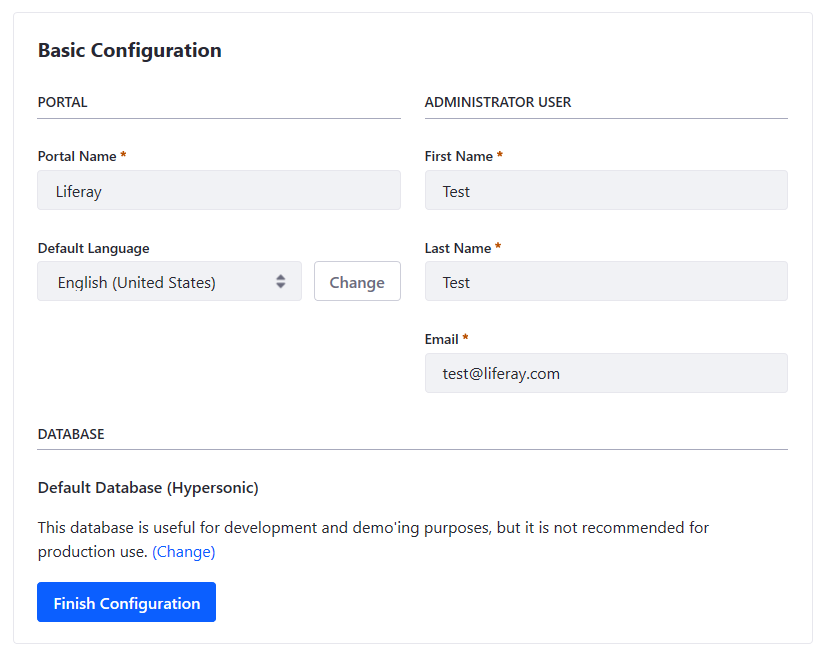
\includegraphics{./images/basic-configuration1.png}
\caption{Supply the information for your portal and your portal's
default administrator user on the Basic Configuration page.}
\end{figure}

The Basic Configuration page also includes a checkbox labeled \emph{Add
Sample Data}. If you check this box, sample data is added to your
database. This data includes users, sites, and organizations. The sample
data is for demo purposes. If you're installing Liferay DXP on your own
machine to explore its features, the sample data may be useful. If,
however, you're installing Liferay DXP on a real server, start with a
clean system.

Once you've filled out the form, click \emph{Finish Configuration}. The
setup wizard creates a \texttt{portal-setup-wizard.properties} file
which stores the settings that you entered. When you begin customizing
your portal's configuration, however, use the
\texttt{portal-ext.properties} file you created earlier. All the
possible properties that can be placed in this file are documented in
\href{http://docs.liferay.com/portal/7.0/propertiesdoc}{our reference
documentation}.

\noindent\hrulefill

\textbf{Tip:} The wizard is an extremely helpful tool, especially if
you're setting up Liferay DXP for the first time. If you're a veteran
and you already have your various properties set up, you can disable the
setup wizard. If you disable the setup wizard, you must configure
everything manually from the \texttt{portal-ext.properties} file. To
disable the setup wizard, enter \texttt{setup.wizard.enabled=false} in
your \texttt{portal-ext.properties} file. Note that property values in
\texttt{portal-setup-wizard.properties} (the file created in Liferay
Home by the setup wizard) override property values in
\texttt{portal-ext.properties}.

\noindent\hrulefill

After you've entered the information requested by the Basic
Configuration page, the home page appears. You should set up your mail
configuration next.

\subsection{Configuring Mail}\label{configuring-mail}

Log in as the administrative user you created in the setup wizard. Click
the menu icon and then go to Control Panel → Server Administration →
Mail, and have your mail credentials ready.

Fill out the form. You're asked for the following information:

\textbf{Incoming POP Server:} The hostname for a server running the Post
Office Protocol. Liferay DXP checks this mailbox for incoming messages,
such as message board replies.

\textbf{Incoming Port:} The port on which the POP server is listening.

\textbf{Use a Secure Network Connection:} Use an encrypted connection
when connecting to the POP server.

\textbf{User Name:} The user ID Liferay DXP should use to log into the
POP server.

\textbf{Password:} The password Liferay DXP should use to log into the
POP server.

\textbf{Outgoing SMTP Server:} The hostname for a server running the
Simple Mail Transfer Protocol. Liferay DXP uses this server to send
emails, such as password change emails and other notifications.

\textbf{Outgoing Port:} The port on which the SMTP server is listening.

\textbf{Use a Secure Network Connection:} Use an encrypted connection
when connecting to the SMTP server.

\textbf{User Name:} The user ID Liferay DXP should use to log into the
SMTP server.

\textbf{Password:} The password Liferay DXP should use to log into the
SMTP server.

\textbf{Manually specify additional JavaMail properties to override the
above configuration:} If there are additional properties you need to
specify, supply them here.

When you're finished setting up your mail configuration, click
\emph{Save}.

Your next step is to convert the search implementation from its default
demo mode into a production-ready mode.

\section{Installing Liferay DXP
Manually}\label{installing-liferay-dxp-manually}

The easiest way to install Liferay DXP is to
\href{/docs/7-1/deploy/-/knowledge_base/d/installing-liferay}{use a
bundle}. However, this is not always possible. Some organizations have
an existing infrastructure into which Liferay DXP must be installed.
Other organizations have standardized on a particular application
server. Liferay DXP works well with many leading application servers.
Before you get started, note that there are two distinct approaches to
managing Liferay DXP's data source and mail session. All these topics
are covered:

\begin{itemize}
\tightlist
\item
  \hyperref[using-data-sources]{Using data sources}
\item
  \hyperref[using-mail-sessions]{Using mail sessions}
\item
  \hyperref[manual-configuration]{Manual configuration for data sources
  and mail sessions}
\end{itemize}

Start with data sources.

\subsection{Using Data Sources}\label{using-data-sources}

Liferay DXP provides two ways to configure your data source:

\begin{itemize}
\tightlist
\item
  Use Liferay DXP's built-in data source
\item
  Use your application's server's JNDI data source
\end{itemize}

We recommend the built-in data source. Liferay DXP's data source is
configured by properties set in a properties file. By default, you can
enter database connection information on the
\href{/docs/7-1/deploy/-/knowledge_base/d/installing-liferay\#using-the-setup-wizard}{Basic
Configuration page} that appears when Liferay DXP starts for the first
time. The Setup Wizard stores the information you entered in a
configuration file called \texttt{portal-setup-wizard.properties} in
your
\href{/docs/7-1/deploy/-/knowledge_base/d/installing-liferay\#liferay-home}{Liferay
Home} folder. The built-in data source uses this information to connect
to the database.

Although using the built-in data source is recommended, that's not the
only option. You might prefer to use the data source your application
server provides. In this case, a JNDI lookup provides a handle to the
data source and the application server manages the connection pools.

To configure your application server's data source, you must create your
own configuration file and skip the setup wizard. Since you'd be
creating this file \emph{after} the wizard anyway, this isn't a big
deal. The \hyperref[manual-configuration]{Manual Configuration} section
below demonstrates configuring a JNDI data source.

Since mail sessions are configured similarly to data sources, they're
next.

\subsection{Using Mail Sessions}\label{using-mail-sessions}

Liferay DXP uses SMTP to send mail. As with databases, you have two ways
to configure your mail server:

\begin{itemize}
\tightlist
\item
  Use Liferay DXP's built-in mail session
\item
  Use your application server's mail session
\end{itemize}

Using the built-in mail session is recommended. After you've started
Liferay DXP, you can configure a mail server through the Control Panel.
The default configuration is a mail server on the same machine running
Liferay DXP. If this is not your configuration, you must modify the
defaults. To do this, use a \texttt{portal-ext.properties} file in your
Liferay Home folder (see below).

To use your application server's mail session, you must create it in
your application server. Once you've created a mail session, you can
point Liferay DXP to it through your \texttt{portal-ext.properties} file
or through the Control Panel.

If you plan to use Liferay DXP to manage both your database connection
and mail session, enter your database connection information on the
Basic Configuration page when Liferay DXP first starts, and then enter
your mail server information through the Control Panel.

If you plan to let your application server manage your database
connection or your mail server, you can't use Liferay DXP's setup
wizard: you must follow the instructions in the
\hyperref[manual-configuration]{Manual Configuration} section below.

The installation articles for each application server also include
instructions for configuring your application server to manage the
database connection and mail server.

\subsection{Manual Configuration}\label{manual-configuration}

To have your application server manage your database connection or mail
server (or both), you must manually create this configuration. Create a
text file called \texttt{portal-ext.properties} in your Liferay Home
folder. This file overrides the default properties.

To use your application server's data source, create a connection pool
in your application server that points to your database. The connection
pool should be called \texttt{jdbc/LiferayPool}. This is spelled out for
each application server in its article. To tell Liferay DXP to use your
\texttt{jdbc/LiferayPool} connection pool, add the following directive
to your \texttt{portal-ext.properties} file:

\begin{verbatim}
jdbc.default.jndi.name=jdbc/LiferayPool
\end{verbatim}

Next, install Liferay DXP according to the article for your application
server. Once it's installed, you can set up the mail configuration.

You should use the Control Panel to create the mail configuration. Go to
\emph{Control Panel → Configuration → Server Administration → Mail} and
enter your settings for your mail session settings.

You can also configure this with the \texttt{portal-ext.properties}
file, which lets you do the configuration once and then copy the
configuration file to multiple machines. To use the built-in mail
session, use the following properties and customize their values for
your environment:

\begin{verbatim}
mail.session.mail.pop3.host=localhost
mail.session.mail.pop3.password=
mail.session.mail.pop3.port=110
mail.session.mail.pop3.user=
mail.session.mail.smtp.auth=false
mail.session.mail.smtp.host=localhost
mail.session.mail.smtp.password=
mail.session.mail.smtp.port=25
mail.session.mail.smtp.user=
mail.session.mail.store.protocol=pop3
mail.session.mail.transport.protocol=smtp
\end{verbatim}

To use your application server's mail session, create it first. Then
specify it in the \texttt{portal-ext.properties} file:

\begin{verbatim}
mail.session.jndi.name=mail/MailSession
\end{verbatim}

When you're finished, save the file.

\subsection{Logging}\label{logging}

After deploying Liferay DXP, you may see excessive warnings and log
messages, such as the ones below, involving \texttt{PhaseOptimizer}.
These are benign and can be ignored. Make sure to adjust your app
server's logging level or log filters to avoid excessive benign log
messages.

\begin{verbatim}
May 02, 2018 9:12:27 PM com.google.javascript.jscomp.PhaseOptimizer$NamedPass process
WARNING: Skipping pass gatherExternProperties
May 02, 2018 9:12:27 PM com.google.javascript.jscomp.PhaseOptimizer$NamedPass process
WARNING: Skipping pass checkControlFlow
May 02, 2018 9:12:27 PM com.google.javascript.jscomp.PhaseOptimizer$NamedPass process
INFO: pass supports: [ES3 keywords as identifiers, getters, reserved words as properties, setters, string continuation, trailing comma, array pattern rest, arrow function, binary literal, block-scoped function declaration, class, computed property, const declaration, default parameter, destructuring, extended object literal, for-of loop, generator, let declaration, member declaration, new.target, octal literal, RegExp flag 'u', RegExp flag 'y', rest parameter, spread expression, super, template literal, modules, exponent operator (**), async function, trailing comma in param list]
current AST contains: [ES3 keywords as identifiers, getters, reserved words as properties, setters, string continuation, trailing comma, array pattern rest, arrow function, binary literal, block-scoped function declaration, class, computed property, const declaration, default parameter, destructuring, extended object literal, for-of loop, generator, let declaration, member declaration, new.target, octal literal, RegExp flag 'u', RegExp flag 'y', rest parameter, spread expression, super, template literal, exponent operator (**), async function, trailing comma in param list, object literals with spread, object pattern rest]
\end{verbatim}

\section{Installing Liferay DXP on
Tomcat}\label{installing-liferay-dxp-on-tomcat}

7.0 bundled with Tomcat 9 is available on the
\href{https://help.liferay.com/hc}{Help Center} (DXP) or
\href{https://www.liferay.com/downloads}{Liferay Downloads} (Portal CE).
The Tomcat bundle contains JARs, scripts, and configuration files
required for installing Liferay DXP on a clean Tomcat 9 application
server. Copying these files from a Liferay DXP Tomcat bundle facilitates
installing Liferay DXP on Tomcat.

Whether you copy bundle files (recommended) or download and create the
files, you must download these \emph{Additional Files} for
\href{https://help.liferay.com/hc}{DXP} or
\href{https://www.liferay.com/downloads-community}{Portal CE}:

\begin{itemize}
\tightlist
\item
  Liferay DXP WAR file
\item
  Dependencies ZIP file
\item
  OSGi Dependencies ZIP file
\end{itemize}

Liferay DXP requires a Java JDK 8 or 11.

\noindent\hrulefill

\textbf{Note:} Please see
\href{https://www.liferay.com/documents/10182/246659966/Liferay+DXP+7.1+Compatibility+Matrix.pdf/c8805b72-c693-1f26-3f2d-731ffc301366}{the
compatibility matrix} for information on supported JDKs, databases, and
environments.

\noindent\hrulefill

Here are the basic steps for installing Liferay DXP on Tomcat:

\begin{itemize}
\tightlist
\item
  \hyperref[installing-dependencies]{Installing dependencies to your
  application server}
\item
  \hyperref[configuring-tomcat]{Configuring your application server for
  Liferay DXP}
\item
  \hyperref[deploying-liferay]{Deploying the Liferay DXP WAR file to
  your application server}
\end{itemize}

\href{/docs/7-1/deploy/-/knowledge_base/d/installing-liferay\#liferay-home}{\emph{Liferay
Home}} is the folder containing your Tomcat server folder. After
installing and deploying Liferay DXP, Liferay Home contains
\texttt{data}, \texttt{deploy}, \texttt{license}, and \texttt{osgi}
folders. \texttt{\$TOMCAT\_HOME} refers to your Tomcat server folder. It
is usually named \texttt{tomcat-{[}version{]}} or
\texttt{apache-tomcat-{[}version{]}}.

\subsection{Installing Dependencies}\label{installing-dependencies}

Liferay DXP depends on many JARs included by Liferay DXP Tomcat bundle.
Some of the bundle's JARs are not strictly required but can still be
useful. If you don't have a bundle, download the required JARs from
third-parties, as described below.

\begin{enumerate}
\def\labelenumi{\arabic{enumi}.}
\item
  Unzip the Dependencies ZIP file contents in the
  \texttt{\$TOMCAT\_HOME/lib/ext} folder (create this folder if it
  doesn't exist).
\item
  Download a database driver \texttt{.jar} file and copy it to the
  \texttt{\$CATALINA\_BASE/lib/ext} folder. For a list of supported
  databases, see Liferay's
  \href{https://web.liferay.com/documents/14/21598941/Liferay+DXP+7.1+Compatibility+Matrix/9f9c917a-c620-427b-865d-5c4b4a00be85}{compatibility
  matrix}
\item
  Download the following JARs or copy them from a Liferay DXP Tomcat
  bundle to the \texttt{\$TOMCAT\_HOME/lib/ext} folder:

  \begin{itemize}
  \tightlist
  \item
    \href{http://www.oracle.com/technetwork/java/javase/jaf-136260.html}{\texttt{activation.jar}}
  \item
    \href{http://mvnrepository.com/artifact/javax.ccpp/ccpp/1.0}{\texttt{ccpp.jar}}
  \item
    \href{http://www.oracle.com/technetwork/java/docs-136352.html}{\texttt{jms.jar}}
  \item
    \href{http://www.oracle.com/technetwork/java/javaee/jta/index.html}{\texttt{jta.jar}}
  \item
    \href{http://mvnrepository.com/artifact/com.beetstra.jutf7/jutf7}{\texttt{jutf7.jar}}
  \item
    \href{http://www.oracle.com/technetwork/java/index-138643.html}{\texttt{mail.jar}}
  \item
    \href{http://mvnrepository.com/artifact/org.eclipse.persistence/javax.persistence/2.1.1}{\texttt{persistence.jar}}
  \item
    \href{http://mvnrepository.com/artifact/com.liferay.portal/com.liferay.support.tomcat}{\texttt{support-tomcat.jar}}
  \end{itemize}
\item
  Unzip the OSGi Dependencies ZIP file contents in the
  \texttt{{[}Liferay\ Home{]}/osgi} folder (create this folder if it
  doesn't exist).
\end{enumerate}

\subsection{Configuring Tomcat}\label{configuring-tomcat}

Configuring Tomcat to run Liferay DXP includes these things:

\begin{itemize}
\tightlist
\item
  Setting environment variables
\item
  Specifying a web application context for Liferay DXP
\item
  Setting properties and descriptors
\end{itemize}

Optionally, you can configure Tomcat to manage these things for Liferay
DXP:

\begin{itemize}
\tightlist
\item
  \hyperref[database-configuration]{Data source}
\item
  \hyperref[mail-configuration]{Mail session}
\end{itemize}

Start with configuring Tomcat to run Liferay DXP.

\begin{enumerate}
\def\labelenumi{\arabic{enumi}.}
\item
  If you have a Liferay DXP Tomcat bundle, copy the \texttt{setenv.bat}
  and \texttt{setenv.sh} files from it to your
  \texttt{\$CATALINA\_BASE/bin} folder. If not, create these scripts.

  The scripts set JVM options for Catalina, which is Tomcat's servlet
  container. Among these options is the location of the Java runtime
  environment. If this environment is not available on your server
  globally, you must set its location in in these files so Tomcat can
  run. Do this by pointing the \texttt{JAVA\_HOME} environment variable
  to a Liferay DXP-supported JRE:

\begin{verbatim}
export JAVA_HOME=/usr/lib/jvm/java-8-jdk
export PATH=$JAVA_HOME/bin:$PATH
\end{verbatim}

  Then configure Catalina's JVM options to support Liferay DXP.

  Unix:

\begin{verbatim}
CATALINA_OPTS="$CATALINA_OPTS -Dfile.encoding=UTF-8 -Djava.net.preferIPv4Stack=true -Dorg.apache.catalina.loader.WebappClassLoader.ENABLE_CLEAR_REFERENCES=false -Duser.timezone=GMT -Xmx2048m -XX:MaxMetaspaceSize=512m"
\end{verbatim}

  Windows:

\begin{verbatim}
set "CATALINA_OPTS=%CATALINA_OPTS% -Dfile.encoding=UTF-8 -Djava.net.preferIPv4Stack=true -Dorg.apache.catalina.loader.WebappClassLoader.ENABLE_CLEAR_REFERENCES=false -Duser.timezone=GMT -Xmx2048m -XX:MaxMetaspaceSize=512m"
\end{verbatim}

  This sets the file encoding to UTF-8, prefers an IPv4 stack over IPv6,
  prevents Tomcat from working around garbage collection bugs relating
  to static or final fields (these bugs don't exist in Liferay DXP and
  working around them causes problems with the logging system), sets the
  time zone to GMT, gives the JVM 2GB of RAM, and limits Metaspace to
  500MB.
\end{enumerate}

\noindent\hrulefill

\begin{verbatim}
 **Important:** For Liferay DXP to work properly, the application server JVM
 must use the `GMT` time zone and `UTF-8` file encoding.
\end{verbatim}

\noindent\hrulefill

\noindent\hrulefill

\begin{verbatim}
 **Important:** On JDK 11, the setting `-Djava.locale.providers=JRE,COMPAT,CLDR` is required to display four-digit years. Since JDK 9, the Unicode Common Locale Data Repository (CLDR) is the default locales provider. CLDR does not provide years in a four-digit format (see [LPS-87191](https://issues.liferay.com/browse/LPS-87191)). This setting works around the issue by using JDK 8's default locales provider.
\end{verbatim}

\noindent\hrulefill

\begin{verbatim}
After installation, tune your system (including these JVM options) for
performance. 
\end{verbatim}

\begin{enumerate}
\def\labelenumi{\arabic{enumi}.}
\setcounter{enumi}{1}
\item
  If you have a Liferay DXP Tomcat bundle, copy its
  \texttt{\$CATALINA\_BASE/conf/Catalina/localhost/ROOT.xml} file to the
  corresponding location in your application server. Create the file
  path if it doesn't exist. If you don't have a Liferay DXP Tomcat
  bundle, create a \texttt{ROOT.xml} file.

  The \texttt{ROOT.xml} file specifies a web application context for
  Liferay DXP. \texttt{ROOT.xml} looks like this:

\begin{verbatim}
<Context crossContext="true" path="">

    <!-- JAAS -->

    <!--<Realm
        className="org.apache.catalina.realm.JAASRealm"
        appName="PortalRealm"
        userClassNames="com.liferay.portal.kernel.security.jaas.PortalPrincipal"
        roleClassNames="com.liferay.portal.kernel.security.jaas.PortalRole"
    />-->

    <!--
    Uncomment the following to disable persistent sessions across reboots.
    -->

    <!--<Manager pathname="" />-->

    <!--
    Uncomment the following to not use sessions. See the property
    "session.disabled" in portal.properties.
    -->

    <!--<Manager className="com.liferay.support.tomcat.session.SessionLessManagerBase" />-->

    <Resources>
        <PreResources
            base="${catalina.base}/lib/ext/portal"
            className="com.liferay.support.tomcat.webresources.ExtResourceSet"
            webAppMount="/WEB-INF/lib"
        />
    </Resources>
</Context>
\end{verbatim}

  Setting \texttt{crossContext="true"} lets multiple web applications
  use the same class loader. This configuration includes commented
  instructions and tags for configuring a JAAS realm, disabling
  persistent sessions, and disabling sessions entirely.
\item
  Provide Catalina access to the JARs in
  \texttt{\$CATALINA\_BASE/lib/ext} by opening your
  \texttt{\$CATALINA\_BASE/conf/catalina.properties} file and appending
  this value to the \texttt{common.loader} property:

\begin{verbatim}
,"${catalina.home}/lib/ext/global","${catalina.home}/lib/ext/global/*.jar","${catalina.home}/lib/ext","${catalina.home}/lib/ext/*.jar"
\end{verbatim}
\item
  Make sure to use UTF-8 URI encoding consistently. If you have a
  Liferay DXP Tomcat bundle, copy the
  \texttt{\$CATALINA\_BASE/conf/server.xml} file to your server. If not,
  open your \texttt{\$CATALINA\_BASE/conf/server.xml} file and add the
  attribute \texttt{URIEncoding="UTF-8"} to HTTP and AJP connectors that
  use \texttt{redirectPort=8443}. Here are examples:

  Old:

\begin{verbatim}
<Connector port="8080" protocol="HTTP/1.1" connectionTimeout="20000" redirectPort="8443" />
\end{verbatim}

  New:

\begin{verbatim}
<Connector port="8080" protocol="HTTP/1.1" connectionTimeout="20000" redirectPort="8443" URIEncoding="UTF-8" />
\end{verbatim}

  Old:

\begin{verbatim}
<Connector port="8009" protocol="AJP/1.3" redirectPort="8443" />
\end{verbatim}

  New:

\begin{verbatim}
<Connector port="8009" protocol="AJP/1.3" redirectPort="8443" URIEncoding="UTF-8" />
\end{verbatim}
\item
  If you're on Unix, Linux, or Mac OS, make the shell scripts in your
  \texttt{\$CATALINA\_HOME/bin} and \texttt{\$CATALINA\_BASE/bin}
  folders executable by running this command in each folder:

  \texttt{chmod\ a+x\ *.sh}
\end{enumerate}

\textbf{Checkpoint:}

Your application server is configured to run Liferay DXP.

\begin{enumerate}
\def\labelenumi{\arabic{enumi}.}
\item
  The file encoding, user time-zone, and preferred protocol stack are
  set in \texttt{setenv.sh}.
\item
  The default memory available and Metaspace limit are set.
\item
  \texttt{\$CATALINA\_BASE/conf/Catalina/localhost/ROOT.xml} declares
  the web application context.
\item
  The \texttt{common.loader} property in
  \texttt{\$CATALINA\_BASE/conf/catalina.properties} grants Catalina
  access to the JARs in \texttt{\$CATALINA\_BASE/lib/ext}.
\item
  \texttt{\$CATALINA\_BASE/conf/server.xml} sets UTF-8 encoding.
\item
  The scripts in Tomcat's \texttt{bin} folders are executable.
\end{enumerate}

\subsubsection{Database Configuration}\label{database-configuration}

The easiest way to handle your database configuration is to let Liferay
DXP manage your data source. Liferay DXP's
\href{/docs/7-1/deploy/-/knowledge_base/d/installing-liferay\#using-the-setup-wizard}{Basic
Configuration} page lets you configure Liferay DXP's built-in data
source. If you want to use the built-in data source, skip this section.

If you want Tomcat to manage your data source, follow these steps:

\begin{enumerate}
\def\labelenumi{\arabic{enumi}.}
\item
  Make sure your database server is installed and working. If it's
  installed on a different machine, make sure it's accessible from your
  Liferay DXP machine.
\item
  Open \texttt{\$CATALINA\_BASE/conf/Catalina/localhost/ROOT.xml} and
  add your data source as a \texttt{Resource} in your web application
  \texttt{Context}:

\begin{verbatim}
<Context...>
    ...
    <Resource
        name="jdbc/LiferayPool"
        auth="Container"
        type="javax.sql.DataSource"
        driverClassName="com.mysql.jdbc.Driver"
        url="jdbc:mysql://localhost/lportal?useUnicode=true&amp;characterEncoding=UTF-8"
        username="root"
        password="root"
        maxTotal="100"
        maxIdle="30"
        maxWaitMillis="10000"
    />
</Context>
\end{verbatim}

  The resource definition above is for a MySQL database named
  \texttt{lportal} that has a user named \texttt{root} whose password is
  \texttt{root}. Replace these values with your own.
\item
  In a \texttt{portal-ext.properties} file in your Liferay Home, specify
  your data source:

\begin{verbatim}
jdbc.default.jndi.name=jdbc/LiferayPool
\end{verbatim}
\end{enumerate}

You created a data source for Tomcat to manage and configured Liferay
DXP to use it. Mail session configuration is next.

\subsubsection{Mail Configuration}\label{mail-configuration}

As with database configuration, the easiest way to configure mail is to
let Liferay DXP handle your mail session. If you want to use Liferay
DXP's built-in mail session, skip this section and
\href{/docs/7-1/deploy/-/knowledge_base/d/installing-liferay\#configuring-mail}{configure
the mail session} in the Control Panel.

If you want to manage your mail session with Tomcat, follow these steps:

\begin{enumerate}
\def\labelenumi{\arabic{enumi}.}
\item
  Open \texttt{\$CATALINA\_BASE/conf/Catalina/localhost/ROOT.xml} and
  add your mail session as a \texttt{Resource} in your web application
  \texttt{Context}. Make sure to replace the example mail session values
  with your own.

\begin{verbatim}
<Context...>
    ...
    <Resource
        name="mail/MailSession"
        auth="Container"
        type="javax.mail.Session"
        mail.pop3.host="pop.gmail.com"
        mail.pop3.port="110"
        mail.smtp.host="smtp.gmail.com"
        mail.smtp.port="465"
        mail.smtp.user="user"
        mail.smtp.password="password"
        mail.smtp.auth="true"
        mail.smtp.starttls.enable="true"
        mail.smtp.socketFactory.class="javax.net.ssl.SSLSocketFactory"
        mail.imap.host="imap.gmail.com"
        mail.imap.port="993"
        mail.transport.protocol="smtp"
        mail.store.protocol="imap"
    />
</Context>
\end{verbatim}
\item
  In your \texttt{portal-ext.properties} file in Liferay Home, reference
  your mail session:

\begin{verbatim}
mail.session.jndi.name=mail/MailSession
\end{verbatim}
\end{enumerate}

You've created a mail session for Tomcat to manage and configured
Liferay DXP to use it.

\subsection{Deploying Liferay}\label{deploying-liferay}

Now you're ready to deploy Liferay DXP using the Liferay DXP WAR file.

\begin{enumerate}
\def\labelenumi{\arabic{enumi}.}
\item
  If you are manually installing Liferay DXP on a clean Tomcat server,
  delete the contents of the \texttt{\$CATALINA\_BASE/webapps/ROOT}
  folder. This removes the default Tomcat home page.
\item
  Extract the Liferay DXP \texttt{.war} file to
  \texttt{\$CATALINA\_BASE/webapps/ROOT}.

  It's time to launch Liferay DXP on Tomcat!
\item
  Start Tomcat by navigating to \texttt{\$CATALINA\_HOME/bin} and
  executing \texttt{./startup.sh}. Alternatively, execute
  \texttt{./catalina.sh\ run} to tail Liferay DXP's log file. The log
  audits startup activities and is useful for debugging deployment.
\end{enumerate}

Congratulations on successfully installing and deploying Liferay DXP on
Tomcat!

\noindent\hrulefill

After deploying Liferay DXP, you may see excessive warnings and log
messages, such as the ones below, involving \texttt{PhaseOptimizer}.
These are benign and can be ignored. Make sure to adjust your app
server's logging level or log filters to avoid excessive benign log
messages.

\begin{verbatim}
 May 02, 2018 9:12:27 PM com.google.javascript.jscomp.PhaseOptimizer$NamedPass process
 WARNING: Skipping pass gatherExternProperties
 May 02, 2018 9:12:27 PM com.google.javascript.jscomp.PhaseOptimizer$NamedPass process
 WARNING: Skipping pass checkControlFlow
 May 02, 2018 9:12:27 PM com.google.javascript.jscomp.PhaseOptimizer$NamedPass process
 INFO: pass supports: [ES3 keywords as identifiers, getters, reserved words as properties, setters, string continuation, trailing comma, array pattern rest, arrow function, binary literal, block-scoped function declaration, class, computed property, const declaration, default parameter, destructuring, extended object literal, for-of loop, generator, let declaration, member declaration, new.target, octal literal, RegExp flag 'u', RegExp flag 'y', rest parameter, spread expression, super, template literal, modules, exponent operator (**), async function, trailing comma in param list]
 current AST contains: [ES3 keywords as identifiers, getters, reserved words as properties, setters, string continuation, trailing comma, array pattern rest, arrow function, binary literal, block-scoped function declaration, class, computed property, const declaration, default parameter, destructuring, extended object literal, for-of loop, generator, let declaration, member declaration, new.target, octal literal, RegExp flag 'u', RegExp flag 'y', rest parameter, spread expression, super, template literal, exponent operator (**), async function, trailing comma in param list, object literals with spread, object pattern rest]
\end{verbatim}

\section{Installing Liferay DXP on
Wildfly}\label{installing-liferay-dxp-on-wildfly}

7.0 bundled with Wildfly 11 is available on the
\href{https://help.liferay.com/hc}{Help Center} (DXP) or
\href{https://www.liferay.com/downloads}{Liferay Downloads} (Portal CE).
7.0 supports deployment to Wildfly 10 and Wildfly 11. Even if you want
to manually install Liferay DXP on an existing Wildfly application
server, it can be helpful to download a Liferay DXP Wildfly bundle to
make gathering the dependencies easier. Before proceeding, also download
these \emph{Additional Files} for
\href{https://help.liferay.com/hc}{DXP} or
\href{https://www.liferay.com/downloads-community}{Portal CE}:

\begin{itemize}
\tightlist
\item
  Liferay DXP WAR file
\item
  Dependencies ZIP file
\item
  OSGi Dependencies ZIP file
\end{itemize}

Liferay DXP requires a Java JDK 8 or 11.

\noindent\hrulefill

\textbf{Note:} Please see
\href{https://www.liferay.com/documents/10182/246659966/Liferay+DXP+7.1+Compatibility+Matrix.pdf/c8805b72-c693-1f26-3f2d-731ffc301366}{the
compatibility matrix} for information on supported JDKs, databases, and
environments.

\noindent\hrulefill

Installing Liferay DXP manually takes three steps:

\begin{itemize}
\tightlist
\item
  \hyperref[installing-dependencies]{Installing dependencies to your
  application server}
\item
  \hyperref[configuring-wildfly]{Configuring your application server for
  Liferay DXP}
\item
  \hyperref[deploying-product]{Deploying the Liferay DXP WAR file to
  your application server}
\end{itemize}

\href{/docs/7-1/deploy/-/knowledge_base/d/installing-liferay\#liferay-home}{\emph{Liferay
Home}} is the folder containing your Wildfly server folder. After
installing and deploying Liferay DXP, the Liferay Home folder contains
the Wildfly server folder as well as \texttt{data}, \texttt{deploy},
\texttt{logs}, and \texttt{osgi} folders. \texttt{\$WILDFLY\_HOME}
refers to your Wildfly server folder. It is usually named
\texttt{wildfly-{[}version{]}}.

\subsection{Installing Dependencies}\label{installing-dependencies-1}

Liferay DXP depends on many JARs that are included in the Liferay DXP
Wildfly bundle. Some of the bundle's JARs are not strictly required but
can still be useful. If you don't have a Liferay DXP Wildfly bundle,
download the required JARs from third-parties as described below.

\begin{enumerate}
\def\labelenumi{\arabic{enumi}.}
\item
  Create the folder
  \texttt{\$WILDFLY\_HOME/modules/com/liferay/portal/main} if it doesn't
  exist and extract the dependencies ZIP JARs to it.
\item
  Download your database driver \texttt{.jar} file and copy it into the
  same folder. Please see the
  \href{https://web.liferay.com/documents/14/21598941/Liferay+DXP+7.1+Compatibility+Matrix/9f9c917a-c620-427b-865d-5c4b4a00be85}{compatibility
  matrix} for a list of supported databases.
\item
  Create the file \texttt{module.xml} in the
  \texttt{\$WILDFLY\_HOME/modules/com/liferay/portal/main} folder. In
  the file, declare the portal module and all of its required resources
  and dependencies:

\begin{verbatim}
<?xml version="1.0"?>

<module xmlns="urn:jboss:module:1.0" name="com.liferay.portal">
    <resources>
        <resource-root path="[place your database vendor's JAR file name here]" />
        <resource-root path="[place a Liferay dependencies JAR file name here]" />
        <!-- Add a resource-root element for each Liferay dependencies JAR -->
    </resources>
    <dependencies>
        <module name="javax.api" />
        <module name="javax.mail.api" />
        <module name="javax.servlet.api" />
        <module name="javax.servlet.jsp.api" />
        <module name="javax.transaction.api" />
    </dependencies>
</module>
\end{verbatim}

  Replace
  \texttt{{[}place\ your\ database\ vendor\textquotesingle{}s\ JAR\ file\ name\ here{]}}
  with the driver JAR for your database.

  For each JAR in the Liferay dependencies ZIP, add a
  \texttt{resource-root} element with its \texttt{path} attribute set to
  the JAR name. For example, add a \texttt{resource-root} element like
  this for the \texttt{com.liferay.petra.concurrent.jar} file:

\begin{verbatim}
<resource-root path="com.liferay.petra.concurrent.jar" />
\end{verbatim}
\item
  Create an \texttt{osgi} folder in your Liferay Home folder. Extract
  the OSGi ZIP file that you downloaded into the \texttt{osgi} folder.

  The \texttt{osgi} folder provides the necessary modules for Liferay
  DXP's OSGi runtime.
\end{enumerate}

\textbf{Checkpoint:}

\begin{enumerate}
\def\labelenumi{\arabic{enumi}.}
\tightlist
\item
  The contents of the Dependencies zip have been placed in the
  \texttt{\$WILDFLY\_HOME/modules/com/liferay/portal/main} folder:
\item
  Your database vendor's JDBC driver has been placed in
  \texttt{\$WILDFLY\_HOME/modules/com/liferay/portal/main} folder and
  listed as a dependency.
\item
  The \texttt{module.xml} has listed all JARs in the
  \texttt{\textless{}resource-root\textgreater{}} elements.
\item
  The OSGi dependencies have been unzipped in the \texttt{osgi} folder
  located inside the \texttt{\$\{Liferay.home\}} folder.
\end{enumerate}

\subsection{Running Liferay DXP on Wildfly in Standalone Mode vs.~Domain
Mode}\label{running-liferay-dxp-on-wildfly-in-standalone-mode-vs.-domain-mode}

Wildfly can be launched in either \emph{standalone} mode or
\emph{domain} mode. Domain mode allows multiple application server
instances to be managed from a single control point. A collection of
such application servers is known as a \emph{domain}. For more
information on standalone mode vs.~domain mode, please refer to the
section on this topic in the
\href{https://docs.jboss.org/author/display/WFLY/Admin+Guide\#AdminGuide-Operatingmodes}{Wildfly
Admin Guide}. Liferay DXP fully supports Wildfly in standalone mode but
not in domain mode.

You can run Liferay DXP on Wildfly in domain mode, but this method is
not fully supported. In particular, Liferay DXP's hot-deploy does not
work with a managed deployment, since Wildfly manages the content of a
managed deployment by copying files (exploded or non-exploded). This
prevents JSP hooks and Ext plugins from working as intended. For
example, JSP hooks don't work on Wildfly running in managed domain mode,
since Liferay DXP's JSP override mechanism relies on the application
server. Since both of these features are deprecated, however, you may
not be using them.

The command line interface is recommended for domain mode deployments.

\noindent\hrulefill

\textbf{Note:} This does not prevent Liferay DXP from running in a
clustered environment on multiple Wildfly servers. You can set up a
cluster of Liferay DXP instances running on Wildfly servers running in
standalone mode. Please refer to the chapter of this guide on
\href{/docs/7-1/deploy/-/knowledge_base/d/liferay-clustering}{Liferay
DXP Clustering} for information on setting up a Liferay DXP cluster.

\noindent\hrulefill

\subsection{Configuring Wildfly}\label{configuring-wildfly}

Configuring Wildfly to run Liferay DXP includes these things:

\begin{itemize}
\tightlist
\item
  Setting environment variables
\item
  Setting properties and descriptors
\item
  Removing unnecessary configurations
\end{itemize}

Optionally, you can configure Wildfly to manage Liferay DXP's data
source and mail session.

Start with configuring Wildfly to run Liferay DXP.

Make the following modifications to
\texttt{\$WILDFLY\_HOME/standalone/configuration/standalone.xml}:

\begin{enumerate}
\def\labelenumi{\arabic{enumi}.}
\item
  In the \texttt{\textless{}jsp-config\textgreater{}} tag, set the Java
  VM compatibility for Liferay source and class files. They are
  compatible with Java 8 by default.

\begin{verbatim}
<jsp-config development="true" source-vm="1.8" target-vm="1.8" />
\end{verbatim}
\item
  Locate the closing \texttt{\textless{}/extensions\textgreater{}} tag.
  Directly beneath that tag, insert the following system properties:

\begin{verbatim}
<system-properties>
    <property name="org.apache.catalina.connector.URI_ENCODING" value="UTF-8" />
    <property name="org.apache.catalina.connector.USE_BODY_ENCODING_FOR_QUERY_STRING" value="true" />
</system-properties>
\end{verbatim}
\item
  Add the following \texttt{\textless{}filter-spec\textgreater{}} tag
  within the \texttt{\textless{}console-handler\textgreater{}} tag,
  directly below the
  \texttt{\textless{}level\ name="INFO"/\textgreater{}} tag:

\begin{verbatim}
<filter-spec value="not(any(match(&quot;WFLYSRV0059&quot;),match(&quot;WFLYEE0007&quot;)))" />
\end{verbatim}
\item
  Add a timeout for the deployment scanner by setting
  \texttt{deployment-timeout="360"} as seen in the excerpt below.

\begin{verbatim}
<subsystem xmlns="urn:jboss:domain:deployment-scanner:2.0">
    <deployment-scanner deployment-timeout="360" path="deployments" relative-to="jboss.server.base.dir" scan-interval="5000" runtime-failure-causes-rollback="${jboss.deployment.scanner.rollback.on.failure:false}"/>
</subsystem>
\end{verbatim}
\item
  Add the following JAAS security domain to the security subsystem
  \texttt{\textless{}security-domains\textgreater{}} defined in element
  \texttt{\textless{}subsystem\ \ \ \ \ xmlns="urn:jboss:domain:security:2.0"\textgreater{}}.

\begin{verbatim}
<security-domain name="PortalRealm">
    <authentication>
        <login-module code="com.liferay.portal.kernel.security.jaas.PortalLoginModule" flag="required" />
    </authentication>
</security-domain>
\end{verbatim}
\item
  Remove the two code snippets providing welcome content:

\begin{verbatim}
<location name="/" handler="welcome-content"/>
\end{verbatim}

  and

\begin{verbatim}
<handlers>
    <file name="welcome-content" path="${jboss.home.dir}/welcome-content"/>
</handlers>
\end{verbatim}
\end{enumerate}

\textbf{Checkpoint:}

Before continuing, verify the following properties have been set in the
\texttt{standalone.xml} file:

\begin{enumerate}
\def\labelenumi{\arabic{enumi}.}
\item
  The new \texttt{\textless{}system-property\textgreater{}} is added.
\item
  The new \texttt{\textless{}filter-spec\textgreater{}} is added.
\item
  The \texttt{\textless{}deployment-timeout\textgreater{}} is set to
  \texttt{360}.
\item
  The new \texttt{\textless{}security-domain\textgreater{}} is created.
\item
  Welcome content is removed.
\item
  The \texttt{\textless{}jsp-config\textgreater{}} tag contains its new
  attributes.
\end{enumerate}

Now you must configure your JVM and startup scripts.

In the \texttt{\$WILDFLY\_HOME/bin/} folder, you must make these
modifications to your standalone domain's configuration script file
\texttt{standalone.conf} (\texttt{standalone.conf.bat} on Windows):

\begin{itemize}
\tightlist
\item
  Set the file encoding
\item
  Set the user time-zone
\item
  Set the preferred protocol stack
\item
  Increase the default amount of memory available.
\end{itemize}

Make the following edits as applicable for your operating system:

\textbf{Windows:}

\begin{enumerate}
\def\labelenumi{\arabic{enumi}.}
\item
  Comment out the initial \texttt{JAVA\_OPTS} assignment like this:

\begin{verbatim}
rem set "JAVA_OPTS=-Xms64M -Xmx512M -XX:MetaspaceSize=96M -XX:MaxMetaspaceSize=256m"
\end{verbatim}
\item
  Add the following \texttt{JAVA\_OPTS} assignment one line above the
  \texttt{:JAVA\_OPTS\_SET} line found at end of the file:

\begin{verbatim}
set "JAVA_OPTS=%JAVA_OPTS% -Dfile.encoding=UTF-8 -Djava.net.preferIPv4Stack=true -Djboss.as.management.blocking.timeout=480 -Duser.timezone=GMT -Xmx2048m -XX:MaxMetaspaceSize=512m -XX:MetaspaceSize=200m"
\end{verbatim}
\end{enumerate}

\textbf{Unix:}

\begin{enumerate}
\def\labelenumi{\arabic{enumi}.}
\item
  Below the \texttt{if\ {[}\ "x\$JAVA\_OPTS"\ =\ "x"\ {]};} statement,
  replace this \texttt{JAVA\_OPTS} statement:

\begin{verbatim}
JAVA_OPTS="-Xms64m -Xmx512m -XX:MetaspaceSize=96M -XX:MaxMetaspaceSize=256m -Djava.net.preferIPv4Stack=true"
\end{verbatim}

  with this:

\begin{verbatim}
JAVA_OPTS="-Djava.net.preferIPv4Stack=true"
\end{verbatim}
\item
  Add the following statement to the bottom of the file:

\begin{verbatim}
JAVA_OPTS="$JAVA_OPTS -Dfile.encoding=UTF-8 -Djava.net.preferIPv4Stack=true  -Djboss.as.management.blocking.timeout=480 -Duser.timezone=GMT -Xmx2048m -XX:MaxMetaspaceSize=512m -XX:MetaspaceSize=200m"
\end{verbatim}
\end{enumerate}

\noindent\hrulefill

\textbf{Important:} For Liferay DXP to work properly, the application
server JVM must use the \texttt{GMT} time zone and \texttt{UTF-8} file
encoding.

\noindent\hrulefill

\noindent\hrulefill

\textbf{Important:} On JDK 11, the setting
\texttt{-Djava.locale.providers=JRE,COMPAT,CLDR} is required to display
four-digit years. Since JDK 9, the Unicode Common Locale Data Repository
(CLDR) is the default locales provider. CLDR does not provide years in a
four-digit format (see
\href{https://issues.liferay.com/browse/LPS-87191}{LPS-87191}). This
setting works around the issue by using JDK 8's default locales
provider.

\noindent\hrulefill

\noindent\hrulefill

\textbf{Note:} If you plan on using the IBM JDK with your Wildfly
server, you must complete some additional steps. First, navigate to the
\texttt{\$WILDFLY\_HOME/modules/com/liferay/portal/main/module.xml} file
and insert the following dependency within the
\texttt{\textless{}dependencies\textgreater{}} element:

\begin{verbatim}
 <module name="ibm.jdk" />
\end{verbatim}

Then navigate to the
\texttt{\$WILDFLY\_HOME/modules/system/layers/base/sun/jdk/main/module.xml}
file and insert the following path names inside the
\texttt{\textless{}paths\textgreater{}...\textless{}/paths\textgreater{}}
element:

\begin{verbatim}
 <path name="com/sun/crypto" />
 <path name="com/sun/crypto/provider" />
 <path name="com/sun/org/apache/xml/internal/resolver" />
 <path name="com/sun/org/apache/xml/internal/resolver/tools" />
\end{verbatim}

The added paths resolve issues with deployment exceptions and image
uploading problems.

\noindent\hrulefill

\textbf{Checkpoint:}

At this point, you've finished configuring the application server's JVM
settings.

\begin{enumerate}
\def\labelenumi{\arabic{enumi}.}
\item
  The file encoding, user time-zone, preferred protocol stack have been
  set in the \texttt{JAVA\_OPTS} in the \texttt{standalone.conf.bat}
  file.
\item
  The default amount of memory available has been increased.
\end{enumerate}

The prescribed script modifications are now complete for your Liferay
DXP installation on Wildfly. Next you'll configure your database.

\subsubsection{Database Configuration}\label{database-configuration-1}

The easiest way to handle database configuration is to let Liferay DXP
manage your data source. The
\href{/docs/7-1/deploy/-/knowledge_base/d/installing-liferay\#using-the-setup-wizard}{Basic
Configuration} page lets you configure Liferay DXP's built-in data
source. If you want to use the built-in data source, skip this section.

If you want Wildfly to manage your data source, follow these steps:

\begin{enumerate}
\def\labelenumi{\arabic{enumi}.}
\item
  Add the data source inside the
  \texttt{\$WILDFLY\_HOME/standalone/configuration/standalone.xml}
  file's the \texttt{\textless{}datasources\textgreater{}} element.

\begin{verbatim}
<datasource jndi-name="java:jboss/datasources/ExampleDS" pool-name="ExampleDS" enabled="true" jta="true" use-java-context="true" use-ccm="true">
    <connection-url>[place the URL to your database here]</connection-url>
    <driver>[place the driver name here]</driver>
    <security>
        <user-name>[place your user name here]</user-name>
        <password>[place your password here]</password>
    </security>
</datasource>
\end{verbatim}

  Make sure to replace the database URL, user name, and password with
  the appropriate values.
\end{enumerate}

\noindent\hrulefill

\begin{verbatim}
 **Note:** If you must change your datasource `jndi-name` to something
 different, you must also edit the `datasource` element in the
 `<default-bindings>` tag.
\end{verbatim}

\noindent\hrulefill

\begin{enumerate}
\def\labelenumi{\arabic{enumi}.}
\setcounter{enumi}{1}
\item
  Add the driver to the \texttt{standalone.xml} file's
  \texttt{\textless{}drivers\textgreater{}} element also found within
  the \texttt{\textless{}datasources\textgreater{}} element.

\begin{verbatim}
<drivers>
    <driver name="[name of driver must match name above]" module="com.liferay.portal">
        <driver-class>[place your JDBC driver class here]</driver-class>
    </driver>
</drivers>
\end{verbatim}

  A final data source subsystem that uses MySQL should look like this:

\begin{verbatim}
<subsystem xmlns="urn:jboss:domain:datasources:5.0">
    <datasources>
        <datasource jndi-name="java:jboss/datasources/ExampleDS" pool-name="ExampleDS" enabled="true" jta="true" use-java-context="true" use-ccm="true">
            <connection-url>jdbc:mysql://localhost/lportal</connection-url>
            <driver>mysql</driver>
            <security>
                <user-name>root</user-name>
                <password>root</password>
            </security>
        </datasource>
        <drivers>
            <driver name="mysql" module="com.liferay.portal"/>
        </drivers>
    </datasources>
</subsystem>
\end{verbatim}
\item
  In a \texttt{portal-ext.properties} file in your Liferay Home, specify
  your data source:

\begin{verbatim}
jdbc.default.jndi.name=java:jboss/datasources/ExampleDS
\end{verbatim}
\end{enumerate}

Now that you've configured your data source, the mail session is next.

\subsubsection{Mail Configuration}\label{mail-configuration-1}

As with database configuration, the easiest way to configure mail is to
let Liferay DXP handle your mail session. If you want to use Liferay
DXP's built-in mail session, skip this section and
\href{/docs/7-1/deploy/-/knowledge_base/d/installing-liferay\#configuring-mail}{configure
the mail session} in the Control Panel.

If you want to manage your mail session with Wildfly, follow these
steps:

\begin{enumerate}
\def\labelenumi{\arabic{enumi}.}
\item
  Specify your mail subsystem in the
  \texttt{\$WILDFLY\_HOME/standalone/configuration/standalone.xml} file
  like this:

\begin{verbatim}
<subsystem xmlns="urn:jboss:domain:mail:3.0">
    <mail-session jndi-name="java:jboss/mail/MailSession" name="mail-smtp">
        <smtp-server ssl="true" outbound-socket-binding-ref="mail-smtp" username="USERNAME" password="PASSWORD"/>
   </mail-session>
</subsystem>
...
<socket-binding-group name="standard-sockets" default-interface="public" port-offset="${jboss.socket.binding.port-offset:0}">
...
<outbound-socket-binding name="mail-smtp">
        <remote-destination host="smtp.gmail.com" port="465"/>
    </outbound-socket-binding>
</socket-binding-group>
\end{verbatim}
\item
  In your \texttt{portal-ext.properties} file in Liferay Home, reference
  your mail session:

\begin{verbatim}
mail.session.jndi.name=java:jboss/mail/MailSession
\end{verbatim}
\end{enumerate}

You've got mail! Next, you'll deploy Liferay DXP to your Wildfly app
server.

\subsection{Deploying Liferay DXP}\label{deploying-liferay-dxp-1}

Now you're ready to deploy Liferay DXP using the Liferay DXP WAR file.

\begin{enumerate}
\def\labelenumi{\arabic{enumi}.}
\item
  If the folder \texttt{\$WILDFLY\_HOME/standalone/deployments/ROOT.war}
  already exists in your Wildfly installation, delete all of its
  subfolders and files. Otherwise, create a new folder called
  \texttt{\$WILDFLY\_HOME/standalone/deployments/ROOT.war}.
\item
  Unzip the Liferay DXP \texttt{.war} file into the \texttt{ROOT.war}
  folder.
\item
  To trigger deployment of \texttt{ROOT.war}, create an empty file named
  \texttt{ROOT.war.dodeploy} in your
  \texttt{\$WILDFLY\_HOME/standalone/deployments/} folder. On startup,
  Wildfly detects the presence of this file and deploys it as a web
  application.
\item
  Start the Wildfly application server by navigating to
  \texttt{\$WILDFLY\_HOME/bin} and running \texttt{standalone.bat} or
  \texttt{standalone.sh}.
\end{enumerate}

Congratulations; you've deployed Liferay DXP on Wildfly!

\noindent\hrulefill

After deploying Liferay DXP, you may see excessive warnings and log
messages, such as the ones below, involving \texttt{PhaseOptimizer}.
These are benign and can be ignored. Make sure to adjust your app
server's logging level or log filters to avoid excessive benign log
messages.

\begin{verbatim}
 May 02, 2018 9:12:27 PM com.google.javascript.jscomp.PhaseOptimizer$NamedPass process
 WARNING: Skipping pass gatherExternProperties
 May 02, 2018 9:12:27 PM com.google.javascript.jscomp.PhaseOptimizer$NamedPass process
 WARNING: Skipping pass checkControlFlow
 May 02, 2018 9:12:27 PM com.google.javascript.jscomp.PhaseOptimizer$NamedPass process
 INFO: pass supports: [ES3 keywords as identifiers, getters, reserved words as properties, setters, string continuation, trailing comma, array pattern rest, arrow function, binary literal, block-scoped function declaration, class, computed property, const declaration, default parameter, destructuring, extended object literal, for-of loop, generator, let declaration, member declaration, new.target, octal literal, RegExp flag 'u', RegExp flag 'y', rest parameter, spread expression, super, template literal, modules, exponent operator (**), async function, trailing comma in param list]
 current AST contains: [ES3 keywords as identifiers, getters, reserved words as properties, setters, string continuation, trailing comma, array pattern rest, arrow function, binary literal, block-scoped function declaration, class, computed property, const declaration, default parameter, destructuring, extended object literal, for-of loop, generator, let declaration, member declaration, new.target, octal literal, RegExp flag 'u', RegExp flag 'y', rest parameter, spread expression, super, template literal, exponent operator (**), async function, trailing comma in param list, object literals with spread, object pattern rest]
\end{verbatim}

\section{Installing Liferay DXP on JBoss
EAP}\label{installing-liferay-dxp-on-jboss-eap}

Installing Liferay DXP on JBoss EAP 7.1 takes three steps:

\begin{itemize}
\tightlist
\item
  \hyperref[installing-dependencies]{Installing Liferay DXP dependencies
  to your application server}
\item
  \hyperref[configuring-jboss]{Configuring your application server for
  Liferay DXP}
\item
  \hyperref[deploying-product]{Installing the Liferay DXP WAR file to
  your application server}
\end{itemize}

Before proceeding, download these files for
\href{https://help.liferay.com/hc}{DXP} or
\href{https://www.liferay.com/downloads-community}{Portal CE}:

\begin{itemize}
\tightlist
\item
  Liferay DXP WAR file
\item
  Dependencies ZIP file
\item
  OSGi JARs ZIP file
\end{itemize}

Liferay DXP requires a Java JDK 8 or 11.

\noindent\hrulefill

\textbf{Note:} Please see
\href{https://www.liferay.com/documents/10182/246659966/Liferay+DXP+7.1+Compatibility+Matrix.pdf/c8805b72-c693-1f26-3f2d-731ffc301366}{the
compatibility matrix} for information on supported JDKs, databases, and
environments.

\noindent\hrulefill

\href{/docs/7-1/deploy/-/knowledge_base/d/installing-liferay\#liferay-home}{\emph{Liferay
Home}} is the folder containing your JBoss server folder. After
installing and deploying Liferay DXP, the Liferay Home folder contains
the JBoss server folder as well as \texttt{data}, \texttt{deploy},
\texttt{logs}, and \texttt{osgi} folders. \texttt{\$JBOSS\_HOME} refers
to your JBoss server folder. This folder is usually named
\texttt{jboss-eap-{[}version{]}}.

\subsection{Installing Dependencies}\label{installing-dependencies-2}

Liferay DXP depends on several Liferay-specific and third-party JARs.
Download and install the required JARs as described below.

\begin{enumerate}
\def\labelenumi{\arabic{enumi}.}
\item
  Create the folder
  \texttt{\$JBOSS\_HOME/modules/com/liferay/portal/main} if it doesn't
  exist and extract the Liferay dependencies ZIP JARs to it.
\item
  Download your database driver \texttt{.jar} file and copy it into the
  same folder. Please see the
  \href{https://web.liferay.com/documents/14/21598941/Liferay+DXP+7.1+Compatibility+Matrix/9f9c917a-c620-427b-865d-5c4b4a00be85}{compatibility
  matrix} for a list of supported databases.
\item
  Create the file \texttt{module.xml} in the
  \texttt{\$JBOSS\_HOME/modules/com/liferay/portal/main} folder. In the
  file, declare the portal module and all of its required resources and
  dependencies:

\begin{verbatim}
<?xml version="1.0"?>

<module xmlns="urn:jboss:module:1.0" name="com.liferay.portal">
    <resources>
        <resource-root path="[place your database vendor's JAR file name here]" />
        <resource-root path="[place a Liferay dependencies JAR file name here]" />
        <!-- Add a resource-root element for each Liferay dependencies JAR -->
    </resources>
    <dependencies>
        <module name="javax.api" />
        <module name="javax.mail.api" />
        <module name="javax.servlet.api" />
        <module name="javax.servlet.jsp.api" />
        <module name="javax.transaction.api" />
    </dependencies>
</module>
\end{verbatim}

  Replace
  \texttt{{[}place\ your\ database\ vendor\textquotesingle{}s\ JAR\ file\ name\ here{]}}
  with the driver JAR for your database.

  For each JAR in the Liferay dependencies ZIP, add a
  \texttt{resource-root} element with its \texttt{path} attribute set to
  the JAR name. For example, add a \texttt{resource-root} element like
  this for the \texttt{com.liferay.petra.concurrent.jar} file:

\begin{verbatim}
<resource-root path="com.liferay.petra.concurrent.jar" />
\end{verbatim}
\item
  Create an \texttt{osgi} folder in your Liferay Home folder. Extract
  the OSGi ZIP file that you downloaded into the \texttt{osgi} folder.

  The \texttt{osgi} folder provides the necessary modules for Liferay
  DXP's OSGi runtime.
\end{enumerate}

\textbf{Checkpoint:}

\begin{enumerate}
\def\labelenumi{\arabic{enumi}.}
\tightlist
\item
  The dependencies files have been unzipped into the
  \texttt{\$JBOSS\_HOME/modules/com/liferay/portal/main} folder and a
  database jar.
\item
  The \texttt{module.xml} contains all JARs in the
  \texttt{\textless{}resource-root-path\textgreater{}} elements.
\item
  The \texttt{osgi} dependencies have been unzipped into the
  \texttt{osgi} folder.
\end{enumerate}

\subsection{Running Liferay DXP on JBoss EAP in Standalone Mode
vs.~Domain
Mode}\label{running-liferay-dxp-on-jboss-eap-in-standalone-mode-vs.-domain-mode}

JBoss EAP can be launched in either \emph{standalone} mode or
\emph{domain} mode. Domain mode allows multiple application server
instances to be managed from a single control point. A collection of
such application servers is known as a \emph{domain}. For more
information on standalone mode vs.~domain mode, please refer to the
section on this topic in the
\href{https://access.redhat.com/documentation/en-us/red_hat_jboss_enterprise_application_platform/7.1/html/introduction_to_jboss_eap/overview_of_jboss_eap\#operating_modes}{JBoss
EAP Product Documentation}.

Liferay DXP supports JBoss EAP when it runs in standalone mode but not
when it runs in domain mode. Liferay DXP's hot-deploy does not work with
a managed deployment, since JBoss manages the content of a managed
deployment by copying files (exploded or non-exploded). This prevents
JSP hooks and Ext plugins from working as intended. For example, JSP
hooks don't work on JBoss EAP running in managed domain mode, since
Liferay DXP's JSP override mechanism relies on the application server.
Since both of these features are deprecated, however, you may not be
using them.

The command line interface is recommended for domain mode deployments.

\noindent\hrulefill

\textbf{Note:} This does not prevent Liferay DXP from running in a
clustered environment on multiple JBoss servers. You can set up a
cluster of Liferay DXP instances running on JBoss EAP servers running in
standalone mode. Please refer to the
\href{/docs/7-1/deploy/-/knowledge_base/d/liferay-clustering}{Liferay
DXP Clustering} section for information on setting up a Liferay DXP
cluster.

\noindent\hrulefill

\subsection{Configuring JBoss}\label{configuring-jboss}

Configuring JBoss to run Liferay DXP includes these things:

\begin{itemize}
\tightlist
\item
  Setting environment variables
\item
  Setting properties and descriptors
\item
  Removing unnecessary configurations
\end{itemize}

Optionally, you can configure JBoss to manage these things for Liferay
DXP:

\begin{itemize}
\tightlist
\item
  \hyperref[database-configuration]{Data source}
\item
  \hyperref[mail-configuration]{Mail session}
\end{itemize}

Start with configuring JBoss to run Liferay DXP.

Make the following modifications to
\texttt{\$JBOSS\_HOME/standalone/configuration/standalone.xml}:

\begin{enumerate}
\def\labelenumi{\arabic{enumi}.}
\item
  In the \texttt{\textless{}jsp-configuration\textgreater{}} tag, set
  the Java VM compatibility for Liferay source and class files. They are
  compatible with Java 8 by default.

\begin{verbatim}
<jsp-configuration development="true" source-vm="1.8" target-vm="1.8" />
\end{verbatim}
\item
  Locate the closing \texttt{\textless{}/extensions\textgreater{}} tag.
  Directly beneath that tag, insert these system properties:

\begin{verbatim}
<system-properties>
    <property name="org.apache.catalina.connector.URI_ENCODING" value="UTF-8" />
    <property name="org.apache.catalina.connector.USE_BODY_ENCODING_FOR_QUERY_STRING" value="true" />
</system-properties>
\end{verbatim}
\item
  Add the following \texttt{\textless{}filter-spec\textgreater{}} tag
  within the \texttt{\textless{}console-handler\textgreater{}} tag,
  directly below the
  \texttt{\textless{}level\ name="INFO"/\textgreater{}} tag:

\begin{verbatim}
<filter-spec value="not(any(match(&quot;WFLYSRV0059&quot;),match(&quot;WFLYEE0007&quot;)))" />
\end{verbatim}
\item
  Add a timeout for the deployment scanner by setting
  \texttt{deployment-timeout="360"} as seen in the excerpt below.

\begin{verbatim}
<subsystem xmlns="urn:jboss:domain:deployment-scanner:2.0">
    <deployment-scanner deployment-timeout="360" path="deployments" relative-to="jboss.server.base.dir" scan-interval="5000"/>
</subsystem>
\end{verbatim}
\item
  Add the following JAAS security domain to the security subsystem
  \texttt{\textless{}security-domains\textgreater{}} defined in element
  \texttt{\textless{}subsystem\ \ \ \ \ xmlns="urn:jboss:domain:security:2.0"\textgreater{}}.

\begin{verbatim}
<security-domain name="PortalRealm">
    <authentication>
        <login-module code="com.liferay.portal.kernel.security.jaas.PortalLoginModule" flag="required" />
    </authentication>
</security-domain>
\end{verbatim}
\item
  Remove the two code snippets providing welcome content:

\begin{verbatim}
<location name="/" handler="welcome-content"/>
\end{verbatim}

  and

\begin{verbatim}
<handlers>
    <file name="welcome-content" path="${jboss.home.dir}/welcome-content"/>
</handlers>
\end{verbatim}
\item
  Find the \texttt{\textless{}jsp-config/\textgreater{}} tag and set the
  \texttt{development}, \texttt{source-vm}, and \texttt{target-vm}
  attributes in the tag. Once finished, the tag should look like this:

\begin{verbatim}
<jsp-config development="true" source-vm="1.8" target-vm="1.8"/>
\end{verbatim}
\end{enumerate}

\textbf{Checkpoint:}

Before continuing, verify the following properties have been set in the
\texttt{standalone.xml} file:

\begin{enumerate}
\def\labelenumi{\arabic{enumi}.}
\item
  The new \texttt{\textless{}system-property\textgreater{}} is added.
\item
  The new \texttt{\textless{}filter-spec\textgreater{}} is added.
\item
  The \texttt{\textless{}deployment-timeout\textgreater{}} is set to
  \texttt{360}.
\item
  The new \texttt{\textless{}security-domain\textgreater{}} is created.
\item
  Welcome content is removed.
\item
  The \texttt{\textless{}jsp-config\textgreater{}} tag contains its new
  attributes.
\end{enumerate}

Now you should configure your JVM and startup scripts.

In the \texttt{\$JBOSS\_HOME/bin} folder, you must make these
modifications to your standalone domain's configuration script file
\texttt{standalone.conf} (\texttt{standalone.conf.bat} on Windows):

\begin{itemize}
\tightlist
\item
  Set the file encoding to \texttt{UTF-8}
\item
  Set the user time zone to \texttt{GMT}
\item
  Set the preferred protocol stack
\item
  Increase the default amount of memory available.
\end{itemize}

\noindent\hrulefill

\textbf{Important:} For Liferay DXP to work properly, the application
server JVM must use the \texttt{GMT} time zone and \texttt{UTF-8} file
encoding.

\noindent\hrulefill

Make the following edits as applicable to your operating system:

\textbf{Windows}

\begin{enumerate}
\def\labelenumi{\arabic{enumi}.}
\item
  Comment out the initial \texttt{JAVA\_OPTS} assignment as demonstrated
  in the following line:

\begin{verbatim}
rem set "JAVA_OPTS=-Xms1G -Xmx1G -XX:MetaspaceSize=96M -XX:MaxMetaspaceSize=256m"
\end{verbatim}
\item
  Add the following \texttt{JAVA\_OPTS} assignment one line above the
  \texttt{:JAVA\_OPTS\_SET} line found at end of the file:

\begin{verbatim}
set "JAVA_OPTS=%JAVA_OPTS% -Dfile.encoding=UTF-8 -Djava.net.preferIPv4Stack=true -Djboss.as.management.blocking.timeout=480 -Duser.timezone=GMT -Xmx2048m -XX:MaxMetaspaceSize=384m"
\end{verbatim}
\end{enumerate}

\textbf{Unix}

\begin{enumerate}
\def\labelenumi{\arabic{enumi}.}
\item
  Below the \texttt{if\ {[}\ "x\$JAVA\_OPTS"\ =\ "x"\ {]};} statement,
  replace this \texttt{JAVA\_OPTS} statement:

\begin{verbatim}
JAVA_OPTS="-Xms1303m -Xmx1303m -XX:MetaspaceSize=96M -XX:MaxMetaspaceSize=256m -Djava.net.preferIPv4Stack=true
\end{verbatim}

  with this:

\begin{verbatim}
JAVA_OPTS="-Djava.net.preferIPv4Stack=true"
\end{verbatim}
\item
  Add the following statement to the bottom of the file:

\begin{verbatim}
JAVA_OPTS="$JAVA_OPTS -Dfile.encoding=UTF-8 -Djava.net.preferIPv4Stack=true -Djboss.as.management.blocking.timeout=480 -Duser.timezone=GMT -Xmx2048m -XX:MaxMetaspaceSize=512m"
\end{verbatim}
\end{enumerate}

\noindent\hrulefill

\textbf{Important:} On JDK 11, the setting
\texttt{-Djava.locale.providers=JRE,COMPAT,CLDR} is required to display
four-digit years. Since JDK 9, the Unicode Common Locale Data Repository
(CLDR) is the default locales provider. CLDR does not provide years in a
four-digit format (see
\href{https://issues.liferay.com/browse/LPS-87191}{LPS-87191}). This
setting works around the issue by using JDK 8's default locales
provider.

\noindent\hrulefill

\noindent\hrulefill

\textbf{Note:} If you plan on using the IBM JDK with your JBoss server,
you must complete some additional steps. First, navigate to the
\texttt{\$JBOSS\_HOME/modules/com/liferay/portal/main/module.xml} file
and insert the following dependency within the
\texttt{\textless{}dependencies\textgreater{}} element:

\begin{verbatim}
 <module name="ibm.jdk" />
\end{verbatim}

Then navigate to the
\texttt{\$JBOSS\_HOME/modules/system/layers/base/sun/jdk/main/module.xml}
file and insert the following path names inside the
\texttt{\textless{}paths\textgreater{}...\textless{}/paths\textgreater{}}
element:

\begin{verbatim}
 <path name="com/sun/crypto" />
 <path name="com/sun/crypto/provider" />
 <path name="com/sun/image/codec/jpeg" />
 <path name="com/sun/org/apache/xml/internal/resolver" />
 <path name="com/sun/org/apache/xml/internal/resolver/tools" />
\end{verbatim}

The added paths resolve issues with portal deployment exceptions and
image uploading problems.

\noindent\hrulefill

\textbf{Checkpoint:}

At this point, you've finished configuring the application server's JVM
settings.

\begin{enumerate}
\def\labelenumi{\arabic{enumi}.}
\item
  The file encoding, user time-zone, preferred protocol stack have been
  set in the \texttt{JAVA\_OPTS} in the \texttt{standalone.conf.bat}
  file.
\item
  The default amount of memory available has been increased.
\end{enumerate}

The prescribed script modifications are now complete for your Liferay
DXP installation on JBoss. Next you'll configure the database and mail.

\subsection{Database Configuration}\label{database-configuration-2}

The easiest way to handle your database configuration is to let Liferay
DXP manage your data source. The
\href{/docs/7-1/deploy/-/knowledge_base/d/installing-liferay\#using-the-setup-wizard}{Basic
Configuration} page lets you configure Liferay DXP's built-in data
source. If you want to use the built-in data source, skip this section.

If you want JBoss to manage your data source, follow these steps:

\begin{enumerate}
\def\labelenumi{\arabic{enumi}.}
\item
  Add the data source inside the
  \texttt{\$JBOSS\_HOME/standalone/configuration/standalone.xml} file's
  the \texttt{\textless{}datasources\textgreater{}} element.

\begin{verbatim}
<datasource jndi-name="java:jboss/datasources/ExampleDS" pool-name="ExampleDS" enabled="true" jta="true" use-java-context="true" use-ccm="true">
    <connection-url>[place the URL to your database here]</connection-url>
    <driver>[place the driver name here]</driver>
    <security>
        <user-name>[place your user name here]</user-name>
        <password>[place your password here]</password>
    </security>
</datasource>
\end{verbatim}

  Make sure to replace the database URL, user name, and password with
  the appropriate values.
\end{enumerate}

\noindent\hrulefill

\begin{verbatim}
 **Note:** If you must change your datasource `jndi-name` to something
 different, you must also edit the `datasource` element in the
 `<default-bindings>` tag.
\end{verbatim}

\noindent\hrulefill

\begin{enumerate}
\def\labelenumi{\arabic{enumi}.}
\setcounter{enumi}{1}
\item
  Add the driver to the \texttt{standalone.xml} file's
  \texttt{\textless{}drivers\textgreater{}} element also found within
  the \texttt{\textless{}datasources\textgreater{}} element.

\begin{verbatim}
<drivers>
    <driver name="[name of driver must match name above]" module="com.liferay.portal">
        <driver-class>[place your JDBC driver class here]</driver-class>
    </driver>
</drivers>
\end{verbatim}

  A final data source subsystem that uses MySQL should look like this:

\begin{verbatim}
<subsystem xmlns="urn:jboss:domain:datasources:5.0">
    <datasources>
        <datasource jndi-name="java:jboss/datasources/ExampleDS" pool-name="ExampleDS" enabled="true" jta="true" use-java-context="true" use-ccm="true">
            <connection-url>jdbc:mysql://localhost/lportal</connection-url>
            <driver>mysql</driver>
            <security>
                <user-name>root</user-name>
                <password>root</password>
            </security>
        </datasource>
        <drivers>
            <driver name="mysql" module="com.liferay.portal"/>
        </drivers>
    </datasources>
</subsystem>
\end{verbatim}
\item
  In a \texttt{portal-ext.properties} file in your Liferay Home, specify
  your data source:

\begin{verbatim}
jdbc.default.jndi.name=java:jboss/datasources/ExampleDS
\end{verbatim}
\end{enumerate}

Now that you've configured your data source, the mail session is next.

\subsection{Mail Configuration}\label{mail-configuration-2}

As with database configuration, the easiest way to configure mail is to
let Liferay DXP handle your mail session. If you want to use Liferay
DXP's built-in mail session, skip this section and
\href{/docs/7-1/deploy/-/knowledge_base/d/installing-liferay\#configuring-mail}{configure
the mail session} in the Control Panel.

If you want to manage your mail session with JBoss, follow these steps:

\begin{enumerate}
\def\labelenumi{\arabic{enumi}.}
\item
  Specify your mail subsystem in the
  \texttt{\$WILDFLY\_HOME/standalone/configuration/standalone.xml} file
  like this:

\begin{verbatim}
<subsystem xmlns="urn:jboss:domain:mail:3.0">
    <mail-session jndi-name="java:jboss/mail/MailSession" >
        <smtp-server ssl="true" outbound-socket-binding-ref="mail-smtp">
            <login username="USERNAME" password="PASSWORD"/>
        </smtp-server>
   </mail-session>
</subsystem>
...
<socket-binding-group name="standard-sockets" default-interface="public" port-offset="${jboss.socket.binding.port-offset:0}">
...
<outbound-socket-binding name="mail-smtp">
        <remote-destination host="smtp.gmail.com" port="465"/>
    </outbound-socket-binding>
</socket-binding-group>
\end{verbatim}
\item
  In your \texttt{portal-ext.properties} file in Liferay Home, reference
  your mail session:

\begin{verbatim}
mail.session.jndi.name=java:jboss/mail/MailSession
\end{verbatim}
\end{enumerate}

You've got mail! Next, you'll deploy Liferay DXP to your JBoss app
server.

\subsection{Deploying Liferay DXP}\label{deploying-liferay-dxp-2}

\begin{enumerate}
\def\labelenumi{\arabic{enumi}.}
\item
  If the folder \texttt{\$JBOSS\_HOME/standalone/deployments/ROOT.war}
  already exists in your JBoss installation, delete all of its
  subfolders and files. Otherwise, create a new folder called
  \texttt{\$JBOSS\_HOME/standalone/deployments/ROOT.war}.
\item
  Unzip the Liferay DXP \texttt{.war} file into the \texttt{ROOT.war}
  folder.
\item
  To trigger deployment of \texttt{ROOT.war}, create an empty file named
  \texttt{ROOT.war.dodeploy} in your
  \texttt{\$JBOSS\_HOME/standalone/deployments/} folder. On startup,
  JBoss detects the presence of this file and deploys it as a web
  application.
\item
  Start the JBoss application server by navigating to
  \texttt{\$JBOSS\_HOME/bin} and running \texttt{standalone.bat} or
  \texttt{standalone.sh}.
\end{enumerate}

Congratulations; you've now deployed Liferay DXP on JBoss!

\noindent\hrulefill

After deploying Liferay DXP, you may see excessive warnings and log
messages, such as the ones below, involving \texttt{PhaseOptimizer}.
These are benign and can be ignored. Make sure to adjust your app
server's logging level or log filters to avoid excessive benign log
messages.

\begin{verbatim}
 May 02, 2018 9:12:27 PM com.google.javascript.jscomp.PhaseOptimizer$NamedPass process
 WARNING: Skipping pass gatherExternProperties
 May 02, 2018 9:12:27 PM com.google.javascript.jscomp.PhaseOptimizer$NamedPass process
 WARNING: Skipping pass checkControlFlow
 May 02, 2018 9:12:27 PM com.google.javascript.jscomp.PhaseOptimizer$NamedPass process
 INFO: pass supports: [ES3 keywords as identifiers, getters, reserved words as properties, setters, string continuation, trailing comma, array pattern rest, arrow function, binary literal, block-scoped function declaration, class, computed property, const declaration, default parameter, destructuring, extended object literal, for-of loop, generator, let declaration, member declaration, new.target, octal literal, RegExp flag 'u', RegExp flag 'y', rest parameter, spread expression, super, template literal, modules, exponent operator (**), async function, trailing comma in param list]
 current AST contains: [ES3 keywords as identifiers, getters, reserved words as properties, setters, string continuation, trailing comma, array pattern rest, arrow function, binary literal, block-scoped function declaration, class, computed property, const declaration, default parameter, destructuring, extended object literal, for-of loop, generator, let declaration, member declaration, new.target, octal literal, RegExp flag 'u', RegExp flag 'y', rest parameter, spread expression, super, template literal, exponent operator (**), async function, trailing comma in param list, object literals with spread, object pattern rest]
\end{verbatim}

\section{Installing Liferay DXP on tc
Server}\label{installing-liferay-dxp-on-tc-server}

Installing Liferay DXP on tc server requires these \emph{Additional
Files} for \href{https://help.liferay.com/hc}{DXP} or
\href{https://www.liferay.com/downloads-community}{Portal CE}::

\begin{itemize}
\tightlist
\item
  Liferay DXP WAR file
\item
  Dependencies ZIP file
\item
  OSGi Dependencies ZIP file
\end{itemize}

Liferay DXP requires a Java JDK 8 or 11.

\noindent\hrulefill

\textbf{Note:} Please see
\href{https://www.liferay.com/documents/10182/246659966/Liferay+DXP+7.1+Compatibility+Matrix.pdf/c8805b72-c693-1f26-3f2d-731ffc301366}{the
compatibility matrix} for information on supported JDKs, databases, and
environments.

\noindent\hrulefill

Here are the basic steps for installing Liferay DXP on tc Server:

\begin{itemize}
\item
  Installing Liferay DXP dependencies to your application server
\item
  Configuring your application server for Liferay DXP
\item
  Deploying the Liferay DXP WAR file to your application server
\end{itemize}

\noindent\hrulefill

\textbf{Note:} You'll see the term
\href{/docs/7-1/deploy/-/knowledge_base/d/installing-liferay\#liferay-home}{\emph{Liferay
Home}} used in this installation guide. \emph{Liferay Home} refers to
the folder containing your tc Server instance and some Liferay
DXP-specific folders:. \texttt{data}, \texttt{deploy},
\texttt{licenses}, and \texttt{osgi} folders.

\noindent\hrulefill

\subsection{Creating a tc Server}\label{creating-a-tc-server}

\begin{enumerate}
\def\labelenumi{\arabic{enumi}.}
\item
  Download and unzip a tc Server, available
  \href{https://network.pivotal.io/products/pivotal-tcserver}{here}.
  This is referred to as \texttt{{[}TCSERVER\_INSTANCE\_HOME{]}}.
\item
  Create a folder called \texttt{servers} inside
  \texttt{{[}TCSERVER\_INSTANCE\_HOME{]}}. (e.g.~
  \texttt{/opt/pivotal-tc-server/servers}). This folder becomes
  \emph{Liferay Home} (see note above), and you should not confuse the
  two.
\item
  Next, create an instance called \emph{dxp-server} to deploy Liferay
  DXP. Navigate to the
  \texttt{{[}TCSERVER\_INSTANCE\_HOME{]}/developer-4.0.0.RELEASE} folder
  and run this command:

\begin{verbatim}
tcserver create -i ../servers dxp-server
\end{verbatim}

  By default, new instances are created in the
  \texttt{{[}TCSERVER\_INSTANCE\_HOME{]}/instances} folder. The
  \texttt{-i} specifies where to create the folder. The instance
  location can also be changed via a properties file. See the
  \href{https://tcserver.docs.pivotal.io/4x/docs-tcserver/topics/tcserver-properties-reference.html}{tc
  Server documentation} for more information.
\end{enumerate}

Checkpoint:

\begin{enumerate}
\def\labelenumi{\arabic{enumi}.}
\item
  A new folder called \texttt{servers} has been created.
\item
  A new folder called \texttt{dxp-server} has been created inside the
  \texttt{servers} folder. The following folders have been created
  inside the \texttt{dxp-server} folder:

  \begin{itemize}
  \tightlist
  \item
    \texttt{bin}
  \item
    \texttt{conf}
  \item
    \texttt{lib}
  \item
    \texttt{logs}
  \item
    \texttt{temp}
  \item
    \texttt{webapps}
  \item
    \texttt{work}
  \end{itemize}
\end{enumerate}

Next you can install the required dependencies.

\subsection{Installing Liferay DXP
Dependencies}\label{installing-liferay-dxp-dependencies}

Liferay DXP depends on additional JARs that aren't included with tc
Server by default. There are even more JARs that you'd find in a Liferay
DXP bundle that are not required but can be useful. If you don't have a
Liferay DXP bundle, you can download the required JARs from third
parties, as described below.

\noindent\hrulefill

\textbf{Note:} Many required and useful JARs are pre-installed when you
build Liferay DXP from the source code or
\href{https://web.liferay.com/group/customer/dxp/downloads/7-1}{download
a Liferay DXP bundle}. If you want to acquire all of the JARs that ship
with a Liferay DXP bundle quickly, using one of these sources might save
you time.

\noindent\hrulefill

\begin{enumerate}
\def\labelenumi{\arabic{enumi}.}
\item
  Extract the JARs from the dependencies ZIP to the
  \texttt{{[}TCSERVER\_INSTANCE\_HOME{]}/servers/dxp-server/lib} folder.
\item
  Download the following JARs or copy them from a Liferay DXP bundle to
  the \texttt{{[}TCSERVER\_INSTANCE\_HOME{]}/servers/dxp-server/lib}
  folder:

  \begin{itemize}
  \tightlist
  \item
    \href{http://www.oracle.com/technetwork/java/javase/jaf-136260.html}{\texttt{activation.jar}}
  \item
    \href{http://mvnrepository.com/artifact/javax.ccpp/ccpp/1.0}{\texttt{ccpp.jar}}
  \item
    \href{http://www.oracle.com/technetwork/java/docs-136352.html}{\texttt{jms.jar}}
  \item
    \href{http://www.oracle.com/technetwork/java/javaee/jta/index.html}{\texttt{jta.jar}}
  \item
    \href{http://mvnrepository.com/artifact/com.beetstra.jutf7/jutf7}{\texttt{jutf7.jar}}
  \item
    \href{http://www.oracle.com/technetwork/java/index-138643.html}{\texttt{mail.jar}}
  \item
    \href{http://mvnrepository.com/artifact/org.eclipse.persistence/javax.persistence/2.1.1}{\texttt{persistence.jar}}
  \item
    \href{http://mvnrepository.com/artifact/com.liferay.portal/com.liferay.support.tomcat}{\texttt{support-tomcat.jar}}
  \end{itemize}
\item
  Download a database driver \texttt{.jar} file and copy it to the
  \texttt{{[}TCSERVER\_INSTANCE\_HOME{]}/servers/dxp-server/lib} folder.
  For a list of supported databases, see Liferay's
  \href{https://web.liferay.com/documents/14/21598941/Liferay+DXP+7.1+Compatibility+Matrix/9f9c917a-c620-427b-865d-5c4b4a00be85}{compatibility
  matrix}
\item
  Create an \texttt{osgi} folder in your \emph{Liferay Home}. Extract
  the folders (i.e., \texttt{configs}, \texttt{core}, and more) from
  OSGi ZIP file to the \texttt{osgi} folder. The \texttt{osgi} folder
  provides the necessary modules for Liferay DXP's OSGi runtime.
\end{enumerate}

\subsection{Configuring tc Server}\label{configuring-tc-server}

There are a few configuration edits to make so Liferay DXP runs well on
tc Server. All of these configuration changes should be made in your tc
Server runtime instance.

\begin{enumerate}
\def\labelenumi{\arabic{enumi}.}
\item
  Navigate to the
  \texttt{{[}TCSERVER\_INSTANCE\_HOME{]}/servers/dxp-server/bin} folder.
  In \texttt{setenv.sh} replace this line:

\begin{verbatim}
JVM_OPTS="-Xmx512M -Xss256K"
\end{verbatim}

  with this one

\begin{verbatim}
JVM_OPTS="-Dfile.encoding=UTF-8 -Duser.timezone=GMT -Xmx2048M -Xss512K -XX:MaxMetaspaceSize=512m"
\end{verbatim}

  In \texttt{setenv.bat} replace

\begin{verbatim}
set JVM_OPTS=-Xmx512M -Xss256K
\end{verbatim}

  with

\begin{verbatim}
set JVM_OPTS=-Dfile.encoding=UTF-8 -Duser.timezone=GMT -Xmx2048M -Xss512K -XX:MaxMetaspaceSize=512m
\end{verbatim}
\end{enumerate}

\noindent\hrulefill

\begin{verbatim}
 **Important:** For Liferay DXP to work properly, the application server JVM
 must use the `GMT` time zone and `UTF-8` file encoding.
\end{verbatim}

\noindent\hrulefill

\begin{enumerate}
\def\labelenumi{\arabic{enumi}.}
\setcounter{enumi}{1}
\item
  Next, you should make sure that UTF-8 URI encoding is used
  consistently. Open
  \texttt{{[}TCSERVER\_INSTANCE\_HOME{]}/servers/dxp-server/conf/server.xml}
  and make sure the \texttt{Connector} tag includes setting the
  \texttt{URIEncoding} to \texttt{UTF-8}.

\begin{verbatim}
<Connector acceptCount="100"
           connectionTimeout="20000"
           executor="tomcatThreadPool"
           maxKeepAliveRequests="15"
           port="${bio.http.port}"
           protocol="org.apache.coyote.http11.Http11Protocol"
           redirectPort="${bio.https.port}"
           URIEncoding="UTF-8" />
\end{verbatim}
\item
  If you're installing Liferay DXP and tc Server on Windows, open
  \texttt{{[}TCSERVER\_INSTANCE\_HOME{]}/servers/dxp-server/conf/wrapper.conf}
  and replace

\begin{verbatim}
wrapper.java.additional.8=-Xss256K
\end{verbatim}

  with

\begin{verbatim}
wrapper.java.additional.8=-Xmx2048M
\end{verbatim}

  and add these properties:

\begin{verbatim}
wrapper.java.additional.9=-Xss512K
wrapper.java.additional.10=-XX:MaxMetaspaceSize=256M
wrapper.java.additional.11=-Dfile.encoding=UTF-8
\end{verbatim}
\end{enumerate}

\noindent\hrulefill

\begin{verbatim}
 **Important:** For Liferay DXP to work properly, the application server JVM
 must use the `GMT` time zone and `UTF-8` file encoding. If your Java wrapper
 doesn't already specify the `GMT` time zone, add an entry for it:
 
     wrapper.java.additional.12=-Duser.timezone=GMT
\end{verbatim}

\noindent\hrulefill

\noindent\hrulefill

\begin{verbatim}
 **Important:** On JDK 11, the setting `-Djava.locale.providers=JRE,COMPAT,CLDR` is required to display four-digit years. Since JDK 9, the Unicode Common Locale Data Repository (CLDR) is the default locales provider. CLDR does not provide years in a four-digit format (see [LPS-87191](https://issues.liferay.com/browse/LPS-87191)). This setting works around the issue by using JDK 8's default locales provider.
\end{verbatim}

\noindent\hrulefill

\begin{enumerate}
\def\labelenumi{\arabic{enumi}.}
\setcounter{enumi}{3}
\item
  Finally, open
  \texttt{{[}TCSERVER\_INSTANCE\_HOME{]}/servers/dxp-server/conf/web.xml}
  and add the following configuration after
  \texttt{\textless{}load-on-startup\textgreater{}3\textless{}/load-on-startup\textgreater{}}:

\begin{verbatim}
<init-param>
    <param-name>compilerSourceVM</param-name>
    <param-value>1.8</param-value>
</init-param>
<init-param>
    <param-name>compilerTargetVM</param-name>
    <param-value>1.8</param-value>
</init-param> 
\end{verbatim}
\end{enumerate}

\subsubsection{Database Configuration}\label{database-configuration-3}

The easiest way to handle your database configuration is to let Liferay
DXP manage your data source. If you want to use Liferay DXP's built-in
data source, you can skip this section.

If you want tc Server to manage your data source, follow these steps:

\begin{enumerate}
\def\labelenumi{\arabic{enumi}.}
\item
  Make sure your database server is installed and working. If it's
  installed on a different machine, make sure it's accessible from your
  Liferay DXP machine.
\item
  Add your data source as a resource in the context of your web
  application specified in
  \texttt{{[}TCSERVER\_INSTANCE\_HOME{]}/servers/dxp-server/conf/Catalina/localhost/ROOT.xml}
  (create this file if you don't have it already). An example
  configuration is shown below:

\begin{verbatim}
<Context crossContext="true" path="">
  <Resources>
        <PreResources
            base="${catalina.base}/lib/ext/portal"
            className="com.liferay.support.tomcat.webresources.ExtResourceSet"
            webAppMount="/WEB-INF/lib"
        />
    </Resources>
  <Resource
      name="jdbc/LiferayPool"
      auth="Container"
      type="javax.sql.DataSource"
      driverClassName="com.mysql.jdbc.Driver"
      url="jdbc:mysql://localhost/lportal?useUnicode=true&amp;characterEncoding=UTF-8"
      username="root"
      password="root"
      maxActive="100"
      maxIdle="30"
      maxWait="10000"
  />
</Context>
\end{verbatim}

  The resource definition above is for a MySQL database named
  \texttt{lportal}that has a user named \texttt{root} whose password is
  \texttt{root}. Replace these values with your own.
\item
  In a \texttt{portal-ext.properties} file in Liferay Home, specify your
  data source:

\begin{verbatim}
jdbc.default.jndi.name=jdbc/LiferayPool
\end{verbatim}
\end{enumerate}

Your data source is now configured. Next set up the mail session.

\subsubsection{Mail Configuration}\label{mail-configuration-3}

As with database configuration, the easiest way to configure mail is to
let Liferay DXP handle your mail session. If you want to use Liferay
DXP's built-in mail session, skip this section and
\href{/docs/7-1/deploy/-/knowledge_base/d/installing-liferay\#configuring-mail}{configure
the mail session} in the Control Panel.

If you want to manage your mail session with tc Server, follow these
steps:

\begin{enumerate}
\def\labelenumi{\arabic{enumi}.}
\item
  Edit
  \texttt{{[}TCSERVER\_INSTANCE\_HOME{]}/servers/dxp-server/conf/Catalina/localhost/ROOT.xml}
  and add your mail session as a \texttt{Resource} in your web
  application \texttt{Context}. Make sure to replace the example mail
  session values with your own.

\begin{verbatim}
<Context crossContext="true" path="">
  <Resources>
    <PreResources
      base="${catalina.base}/lib/ext/portal"
      className="com.liferay.support.tomcat.webresources.ExtResourceSet"
      webAppMount="/WEB-INF/lib"
    />
  </Resources>
  ...
  <Resource
      name="mail/MailSession"
      auth="Container"
      type="javax.mail.Session"
      mail.pop3.host="pop.gmail.com"
      mail.pop3.port="110"
      mail.smtp.host="smtp.gmail.com"
      mail.smtp.port="465"
      mail.smtp.user="user"
      mail.smtp.password="password"
      mail.smtp.auth="true"
      mail.smtp.starttls.enable="true"
      mail.smtp.socketFactory.class="javax.net.ssl.SSLSocketFactory"
      mail.imap.host="imap.gmail.com"
      mail.imap.port="993"
      mail.transport.protocol="smtp"
      mail.store.protocol="imap"
  />
</Context>
\end{verbatim}
\item
  In your \texttt{portal-ext.properties} file in Liferay Home, reference
  your mail session:

\begin{verbatim}
mail.session.jndi.name=mail/MailSession
\end{verbatim}
\end{enumerate}

You created a mail session for tc Server to manage and configured
Liferay DXP to use it.

\subsection{Deploying Liferay DXP}\label{deploying-liferay-dxp-3}

Now you're ready to deploy Liferay DXP using your Liferay DXP WAR file.

\begin{enumerate}
\def\labelenumi{\arabic{enumi}.}
\item
  If you are manually installing Liferay DXP on a clean tc Server
  instance, delete the contents of the
  \texttt{{[}TCSERVER\_INSTANCE\_HOME{]}/servers/dxp-server/webapps/ROOT}
  directory. This removes the default home page.
\item
  Extract the Liferay DXP \texttt{.war} file to
  \texttt{{[}TCSERVER\_INSTANCE\_HOME{]}/servers/dxp-server/webapps/ROOT}.

  Now it's time to launch Liferay DXP!
\item
  Start tc Server by navigating to the runtime instance's
  \texttt{{[}TCSERVER\_INSTANCE\_HOME{]}/developer-4.0.0.RELEASE} folder
  and run the following command:

\begin{verbatim}
tcserver run -i ../servers dxp-server
\end{verbatim}
\end{enumerate}

Congratulations on successfully installing and deploying Liferay DXP on
tc Server!

\noindent\hrulefill

After deploying Liferay DXP, you may see excessive warnings and log
messages, such as the ones below, involving \texttt{PhaseOptimizer}.
These are benign and can be ignored. Make sure to adjust your app
server's logging level or log filters to avoid excessive benign log
messages.

\begin{verbatim}
 May 02, 2018 9:12:27 PM com.google.javascript.jscomp.PhaseOptimizer$NamedPass process
 WARNING: Skipping pass gatherExternProperties
 May 02, 2018 9:12:27 PM com.google.javascript.jscomp.PhaseOptimizer$NamedPass process
 WARNING: Skipping pass checkControlFlow
 May 02, 2018 9:12:27 PM com.google.javascript.jscomp.PhaseOptimizer$NamedPass process
 INFO: pass supports: [ES3 keywords as identifiers, getters, reserved words as properties, setters, string continuation, trailing comma, array pattern rest, arrow function, binary literal, block-scoped function declaration, class, computed property, const declaration, default parameter, destructuring, extended object literal, for-of loop, generator, let declaration, member declaration, new.target, octal literal, RegExp flag 'u', RegExp flag 'y', rest parameter, spread expression, super, template literal, modules, exponent operator (**), async function, trailing comma in param list]
 current AST contains: [ES3 keywords as identifiers, getters, reserved words as properties, setters, string continuation, trailing comma, array pattern rest, arrow function, binary literal, block-scoped function declaration, class, computed property, const declaration, default parameter, destructuring, extended object literal, for-of loop, generator, let declaration, member declaration, new.target, octal literal, RegExp flag 'u', RegExp flag 'y', rest parameter, spread expression, super, template literal, exponent operator (**), async function, trailing comma in param list, object literals with spread, object pattern rest]
\end{verbatim}

\section{Installing Liferay DXP on WebLogic 12c
R2}\label{installing-liferay-dxp-on-weblogic-12c-r2}

Although you can install Liferay DXP in a WebLogic Admin Server, this
isn't recommended. It's a best practice to install web apps, including
Liferay DXP, in a WebLogic Managed server. Deploying to a Managed Server
lets you start or shut down Liferay DXP more quickly and facilitates
transitioning into a cluster configuration. This article therefore
focuses on installing Liferay DXP in a Managed Server.

Before getting started, create your Admin and Managed Servers. See
\href{http://www.oracle.com/technetwork/middleware/weblogic/documentation/index.html}{WebLogic's
documentation} for instructions on setting up and configuring Admin and
Managed Servers.

You should also read the following articles to familiarize yourself with
Liferay DXP's general installation steps:

\begin{itemize}
\tightlist
\item
  \href{/docs/7-1/deploy/-/knowledge_base/d/installing-liferay}{Installing
  Liferay DXP}
\item
  \href{/docs/7-1/deploy/-/knowledge_base/d/preparing-for-install}{Preparing
  for Install}
\item
  \href{/docs/7-1/deploy/-/knowledge_base/d/installing-liferay-manually}{Installing
  Liferay DXP Manually}
\end{itemize}

Before proceeding, you must download these \emph{Additional Files} for
\href{https://help.liferay.com/hc}{DXP} or
\href{https://www.liferay.com/downloads-community}{Portal CE}:

\begin{itemize}
\tightlist
\item
  Liferay DXP WAR file
\item
  Dependencies ZIP file
\item
  OSGi Dependencies ZIP file
\end{itemize}

Liferay DXP requires a Java JDK 8 or 11.

\noindent\hrulefill

\textbf{Note:} Please see
\href{https://www.liferay.com/documents/10182/246659966/Liferay+DXP+7.1+Compatibility+Matrix.pdf/c8805b72-c693-1f26-3f2d-731ffc301366}{the
compatibility matrix} for information on supported JDKs, databases, and
environments.

\noindent\hrulefill

Without any further ado, get ready to install Liferay DXP in WebLogic!

\subsection{Configuring WebLogic's Node
Manager}\label{configuring-weblogics-node-manager}

WebLogic's Node Manager starts and stops managed servers.

If you're running WebLogic on a UNIX system other than Solaris or Linux,
use the Java Node Manager, instead of the native version of the Node
Manager, by configuring these Node Manager properties in the
\texttt{domains/your\_domain\_name/nodemanager/nodemanager.properties}
file:

\begin{verbatim}
NativeVersionEnabled=false

StartScriptEnabled=true
\end{verbatim}

\noindent\hrulefill

\textbf{Note:} By default, SSL is used with Node Manager. If you want to
disable SSL during development, for example, set
\texttt{SecureListener=false} in your \texttt{nodemanager.properties}
file.

\noindent\hrulefill

See Oracle's
\href{https://docs.oracle.com/middleware/1212/wls/NODEM/java_nodemgr.htm\#NODEM173}{Configuring
Java Node Manager} documentation for details.

\subsection{Configuring WebLogic}\label{configuring-weblogic}

Configure the JVM and other options in a \texttt{setUserOverridesLate}
WebLogic startup script and in your Managed Server UI.

\begin{enumerate}
\def\labelenumi{\arabic{enumi}.}
\item
  Create a \texttt{setUserOverridesLate.sh} script in
  \texttt{{[}Your\ Domain{]}/bin}.
\item
  Add the following settings.

\begin{verbatim}
export DERBY_FLAG="false"
export JAVA_OPTIONS="${JAVA_OPTIONS} -Dfile.encoding=UTF-8 -Duser.timezone=GMT -da:org.apache.lucene... -da:org.aspectj..."
export JAVA_PROPERTIES="-Dfile.encoding=UTF-8 ${JAVA_PROPERTIES} ${CLUSTER_PROPERTIES}"
export MW_HOME="[place your WebLogic Server folder path here]"
export USER_MEM_ARGS="-Xms512m -Xmx2048m"
export WLS_MEM_ARGS_64BIT="-Xms512m -Xmx2048m"
export WLS_MEM_ARGS_32BIT="-Xms512m -Xmx2048m"
\end{verbatim}
\end{enumerate}

\noindent\hrulefill

\begin{verbatim}
 **Important:** For Liferay DXP to work properly, the application server JVM
 must use the `GMT` time zone and `UTF-8` file encoding.
\end{verbatim}

\noindent\hrulefill

\noindent\hrulefill

\begin{verbatim}
 **Important:** On JDK 11, the setting `-Djava.locale.providers=JRE,COMPAT,CLDR` is required to display four-digit years. Since JDK 9, the Unicode Common Locale Data Repository (CLDR) is the default locales provider. CLDR does not provide years in a four-digit format (see [LPS-87191](https://issues.liferay.com/browse/LPS-87191)). This setting works around the issue by using JDK 8's default locales provider.
\end{verbatim}

\noindent\hrulefill

\begin{verbatim}
The `DERBY_FLAG` setting disables the Derby server built in to WebLogic, as DXP does not require this server.

`JAVA_OPTIONS` sets DXP's UTF-8 requirement, Lucene usage, and Aspect Oriented Programming via AspectJ.

`JAVA_PROPERTIES` also sets DXP's UTF-8 requirement.

Set `MW_HOME` to the folder containing the WebLogic server on the machine. For example,

```bash
export MW_HOME="/Users/ray/Oracle/wls12210"
```
    
The `*_MEM_ARGS` variables set DXP's starting and maximum heap memory capacity.
\end{verbatim}

\begin{enumerate}
\def\labelenumi{\arabic{enumi}.}
\setcounter{enumi}{4}
\item
  You must also ensure that the Node Manager sets Liferay DXP's memory
  requirements when starting the Managed Server. In the Admin Server's
  console UI, navigate to the Managed Server you want to deploy Liferay
  DXP to and select the \emph{Server Start} tab. Enter the following
  parameters into the \emph{Arguments} field:

\begin{verbatim}
-Xmx2048m -XX:MaxMetaspaceSize=512m
\end{verbatim}

  Click \emph{Save} when you're finished.
\end{enumerate}

Next, you'll set some Liferay DXP-specific properties for your Liferay
DXP installation.

\subsection{Setting Liferay DXP
Properties}\label{setting-liferay-dxp-properties}

Before installing Liferay DXP, you must set the
\href{/docs/7-1/deploy/-/knowledge_base/d/installing-liferay\#liferay-home}{\emph{Liferay
Home}} folder's location via the \texttt{liferay.home} property in a
\texttt{portal-ext.properties} file. You can also use this file to
override
\href{https://docs.liferay.com/dxp/portal/7.1-latest/propertiesdoc/portal.properties.html}{other
Liferay DXP properties} that you may need.

First, decide which folder you want to serve as Liferay Home. In
WebLogic, your domain's folder is generally Liferay Home, but you can
choose any folder on your machine. Then create your
\texttt{portal-ext.properties} file and add the \texttt{liferay.home}
property:

\begin{verbatim}
liferay.home=/full/path/to/your/liferay/home/folder
\end{verbatim}

Remember to change this file path to the location on your machine that
you want to serve as Liferay Home.

Now that you've created your \texttt{portal-ext.properties} file, you
must put it inside the Liferay DXP WAR file. Expand the Liferay DXP WAR
file and place \texttt{portal-ext.properties} in the
\texttt{WEB-INF/classes} folder. Later, you can deploy the expanded
archive to WebLogic. Alternatively, you can re-WAR the expanded archive
for later deployment. In either case, Liferay DXP reads your property
settings once it starts up.

If you need to make any changes to \texttt{portal-ext.properties} after
Liferay DXP deploys, you can find it in your domain's
\texttt{autodeploy/ROOT/WEB-INF/classes} folder. Note that the
\texttt{autodeploy/ROOT} folder contains the Liferay DXP deployment.

Next, you'll install Liferay DXP's dependencies.

\subsection{Installing Liferay DXP
Dependencies}\label{installing-liferay-dxp-dependencies-1}

You must now install Liferay DXP's dependencies. Recall that earlier you
downloaded two ZIP files containing these dependencies. Install their
contents now:

\begin{enumerate}
\def\labelenumi{\arabic{enumi}.}
\item
  \texttt{liferay-dxp-dependencies-{[}version{]}.zip}: Unzip this file
  and place its contents in your WebLogic domain's \texttt{lib} folder.
\item
  \texttt{liferay-dxp-osgi-{[}version{]}.zip}: Unzip this file and place
  its contents in the \texttt{{[}Liferay\ Home{]}/osgi} folder (create
  this folder if it doesn't exist).
\item
  Download your database driver \texttt{.jar} file and copy it to your
  domain's \texttt{lib} folder. Please see the
  \href{https://web.liferay.com/documents/14/21598941/Liferay+DXP+7.1+Compatibility+Matrix/9f9c917a-c620-427b-865d-5c4b4a00be85}{compatibility
  matrix} for a list of supported databases.
\end{enumerate}

Next, you'll configure your database.

\subsection{Database Configuration}\label{database-configuration-4}

Use the following procedure if you want WebLogic to manage your database
for Liferay DXP. You can skip this section if you want to use Liferay
DXP's built-in Hypersonic database.

\begin{enumerate}
\def\labelenumi{\arabic{enumi}.}
\item
  Log in to your AdminServer console.
\item
  In the \emph{Domain Structure} tree, find your domain and navigate to
  \emph{Services} → \emph{JDBC} → \emph{Data Sources}.
\item
  To create a new data source, click \emph{New}. Fill in the \emph{Name}
  field with \texttt{Liferay\ Data\ Source} and the \emph{JNDI Name}
  field with \texttt{jdbc/LiferayPool}. Select your database type and
  driver. For example, MySQL is \emph{MySQL's Driver (Type 4)
  Versions:using com.mysql.jdbc.Driver}. Click \emph{Next} to continue.
\item
  Accept the default settings on this page and click \emph{Next} to move
  on.
\item
  Fill in your database information for your MySQL database.
\item
  If using MySQL, add the text
  \texttt{?useUnicode=true\&characterEncoding=UTF-8\&\textbackslash{}useFastDateParsing=false}
  to the URL line and test the connection. If it works, click
  \emph{Next}.
\item
  Select the target for the data source and click \emph{Finish}.
\item
  You must now tell Liferay DXP about the JDBC data source. Create a
  \texttt{portal-ext.propreties} file in your Liferay Home directory,
  and add the line \texttt{jdbc.default.jndi.name=jdbc/LiferayPool}.
\end{enumerate}

Alternatively, you can make the above configuration strictly via
properties in the \texttt{portal-ext.properties} file. To do so, place
the following properties and values in the file. Be sure to change the
\texttt{your*} values with the values appropriate for your database's
configuration (if using MySQL):

\begin{verbatim}
jdbc.default.driverClassName=com.mysql.jdbc.Driver
jdbc.default.url=jdbc:mysql://your.db.ip.address/yourdbname?useUnicode?useUnicode=true&characterEncoding=UTF-8&useFastDateParsing=false
jdbc.default.username=yourdbuser
jdbc.default.password=yourdbpassword
\end{verbatim}

Next, you'll configure your mail session.

\subsection{Mail Configuration}\label{mail-configuration-4}

If you want WebLogic to manage your mail session, use the following
procedure. If you want to use Liferay's built-in mail session
(recommended), skip this section.

\begin{enumerate}
\def\labelenumi{\arabic{enumi}.}
\item
  Start WebLogic and log in to your Admin Server's console.
\item
  Select \emph{Services} → \emph{Mail Sessions} from the \emph{Domain
  Structure} box on the left hand side of your Admin Server's console
  UI.
\item
  Click \emph{New} to begin creating a new mail session.
\item
  Name the session \emph{LiferayMail} and give it the JNDI name
  \texttt{mail/MailSession}. Then fill out the \emph{Session Username},
  \emph{Session Password}, \emph{Confirm Session Password}, and
  \emph{JavaMail Properties} fields as necessary for your mail server.
  See the
  \href{http://docs.oracle.com/middleware/1221/wls/FMWCH/pagehelp/Mailcreatemailsessiontitle.html}{WebLogic
  documentation} for more information on these fields. Click \emph{Next}
  when you're done.
\item
  Choose the Managed Server that you'll install Liferay DXP on, and
  click \emph{Finish}. Then shut down your Managed and Admin Servers.
\item
  With your Managed and Admin servers shut down, add the following
  property to your \texttt{portal-ext.properties} file in Liferay Home:

\begin{verbatim}
mail.session.jndi.name=mail/MailSession
\end{verbatim}

  Liferay DXP references your WebLogic mail session via this property
  setting. If you've already deployed Liferay DXP, you can find your
  \texttt{portal-ext.properties} file in your domain's
  \texttt{autodeploy/ROOT/WEB-INF/classes} folder.
\end{enumerate}

Your changes take effect upon restarting your Managed and Admin servers.

\subsection{Deploying Liferay DXP}\label{deploying-liferay-dxp-4}

As mentioned earlier, although you can deploy Liferay DXP to a WebLogic
Admin Server, you should instead deploy it to a WebLogic Managed Server.
Dedicating the Admin Server to managing other servers that run your apps
is a best practice.

Follow these steps to deploy Liferay DXP to a Managed Server:

\begin{enumerate}
\def\labelenumi{\arabic{enumi}.}
\item
  Make sure the Managed Server you want to deploy Liferay DXP to is shut
  down.
\item
  In your Admin Server's console UI, select \emph{Deployments} from the
  \emph{Domain Structure} box on the left hand side. Then click
  \emph{Install} to start a new deployment.
\item
  Select the Liferay DXP WAR file or its expanded contents on your file
  system. Alternatively, you can upload the WAR file by clicking the
  \emph{Upload your file(s)} link. Click \emph{Next}.
\item
  Select \emph{Install this deployment as an application} and click
  \emph{Next}.
\item
  Select the Managed Server you want to deploy Liferay DXP to and click
  \emph{Next}.
\item
  If the default name is appropriate for your installation, keep it.
  Otherwise, give it a name of your choosing and click \emph{Next}.
\item
  Click \emph{Finish}. After the deployment finishes, click \emph{Save}
  if you want to save the configuration.
\item
  Start the Managed Server where you deployed Liferay DXP. Liferay DXP
  precompiles all the JSPs and then launches.
\end{enumerate}

Nice work! Now you're running Liferay DXP on WebLogic.

\noindent\hrulefill

After deploying Liferay DXP, you may see excessive warnings and log
messages, such as the ones below, involving \texttt{PhaseOptimizer}.
These are benign and can be ignored. Make sure to adjust your app
server's logging level or log filters to avoid excessive benign log
messages.

\begin{verbatim}
 May 02, 2018 9:12:27 PM com.google.javascript.jscomp.PhaseOptimizer$NamedPass process
 WARNING: Skipping pass gatherExternProperties
 May 02, 2018 9:12:27 PM com.google.javascript.jscomp.PhaseOptimizer$NamedPass process
 WARNING: Skipping pass checkControlFlow
 May 02, 2018 9:12:27 PM com.google.javascript.jscomp.PhaseOptimizer$NamedPass process
 INFO: pass supports: [ES3 keywords as identifiers, getters, reserved words as properties, setters, string continuation, trailing comma, array pattern rest, arrow function, binary literal, block-scoped function declaration, class, computed property, const declaration, default parameter, destructuring, extended object literal, for-of loop, generator, let declaration, member declaration, new.target, octal literal, RegExp flag 'u', RegExp flag 'y', rest parameter, spread expression, super, template literal, modules, exponent operator (**), async function, trailing comma in param list]
 current AST contains: [ES3 keywords as identifiers, getters, reserved words as properties, setters, string continuation, trailing comma, array pattern rest, arrow function, binary literal, block-scoped function declaration, class, computed property, const declaration, default parameter, destructuring, extended object literal, for-of loop, generator, let declaration, member declaration, new.target, octal literal, RegExp flag 'u', RegExp flag 'y', rest parameter, spread expression, super, template literal, exponent operator (**), async function, trailing comma in param list, object literals with spread, object pattern rest]
\end{verbatim}

\section{Installing Liferay DXP on
WebSphere}\label{installing-liferay-dxp-on-websphere}

IBM ® WebSphere ® is a trademark of International Business Machines
Corporation, registered in many jurisdictions worldwide.

\noindent\hrulefill

\textbf{Tip:} Throughout this installation and configuration process,
WebSphere prompts you to click \emph{Save} to apply changes to the
Master Configuration. Do so intermittently to save your changes.

\noindent\hrulefill

For Liferay DXP to work correctly, WebSphere 8.5.5 Fix Pack 11 (or
later) or WebSphere 9 (Fix Pack 7 is the latest) must be installed. You
can find more information about this fix pack
\href{http://www-01.ibm.com/support/docview.wss?uid=swg24043005}{here}.

Please also note that Liferay DXP doesn't support the WebSphere
Application Liberty Profile.

You should also read the following articles to familiarize yourself with
Liferay DXP's general installation steps:

\begin{itemize}
\tightlist
\item
  \href{/docs/7-1/deploy/-/knowledge_base/d/preparing-for-install}{Preparing
  for Install}
\item
  \href{/docs/7-1/deploy/-/knowledge_base/d/installing-liferay}{Installing
  Liferay DXP}
\end{itemize}

Note that the
\href{/docs/7-1/deploy/-/knowledge_base/d/installing-liferay\#liferay-home}{\emph{Liferay
Home} folder} is important to the operation of Liferay DXP. In Liferay
Home, Liferay DXP creates certain files and folders that it needs to
run. On WebSphere, Liferay Home is typically
\texttt{{[}Install\ Location{]}/WebSphere/AppServer/profiles/your-profile/liferay}.

Before proceeding, you must download these \emph{Additional Files} for
\href{https://help.liferay.com/hc}{DXP} or
\href{https://www.liferay.com/downloads-community}{Portal CE}::

\begin{itemize}
\tightlist
\item
  Liferay DXP WAR file
\item
  Dependencies ZIP file
\item
  OSGi Dependencies ZIP file
\end{itemize}

Liferay DXP requires a Java JDK 8 or 11.

\noindent\hrulefill

\textbf{Note:} Please see
\href{https://www.liferay.com/documents/10182/246659966/Liferay+DXP+7.1+Compatibility+Matrix.pdf/c8805b72-c693-1f26-3f2d-731ffc301366}{the
compatibility matrix} for information on supported JDKs, databases, and
environments.

\noindent\hrulefill

Without any further ado, get ready to install Liferay DXP in WebSphere!

\subsection{Preparing WebSphere for Liferay
DXP}\label{preparing-websphere-for-liferay-dxp}

When the application server binaries have been installed, start the
\emph{Profile Management Tool} to create a profile appropriate for
Liferay DXP.

\begin{enumerate}
\def\labelenumi{\arabic{enumi}.}
\item
  Click \emph{Create\ldots{}}, choose \emph{Application Server}, and
  then click \emph{Next}.
\item
  Click the \emph{Advanced} profile creation option and then click
  \emph{Next}. You need the advanced profile to specify your own values
  for settings such as the location of the profile and names of the
  profile, node and host, to assign your own ports, or to optionally
  choose whether to deploy the administrative console and sample
  application and also add web-server definitions for IBM HTTP Server.
  See the WebSphere documentation for more information about these
  options.

  \begin{figure}
  \centering
  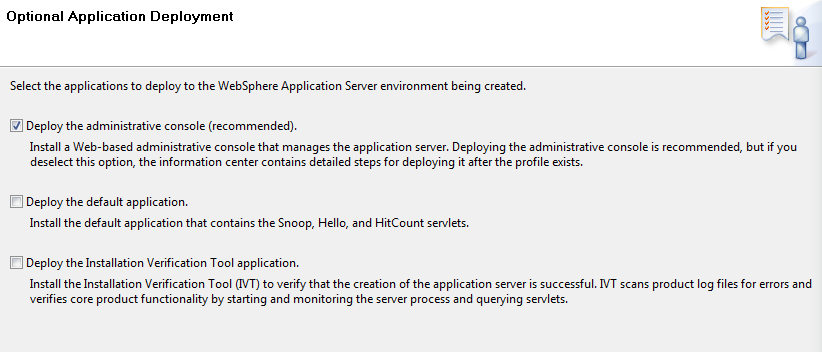
\includegraphics{./images/websphere-01-profile.png}
  \caption{Choose the Advanced profile option to specify your own
  settings.}
  \end{figure}
\item
  Check the box \emph{Deploy the administrative console}. This gives you
  a web-based UI for working with your application server. Skip the
  default applications. You'd only install these on a development
  machine. Click \emph{Next}.
\item
  Set the profile name and location. Ensure you specify a performance
  tuning setting other than \emph{Development}, since you're installing
  a production server. See the WebSphere documentation for more
  information about performance tuning settings. Click \emph{Next}.
\item
  Choose node, server, and host names for your server. These are
  specific to your environment. Click \emph{Next}.
\item
  Administrative security in WebSphere is a way to restrict who has
  access to the administrative tools. You may want to have it enabled in
  your environment so that a user name and password are required to
  administer the WebSphere server. See WebSphere's documentation for
  more information. Click \emph{Next}.
\item
  Each profile needs a security certificate, which comes next in the
  wizard. If you don't have certificates already, choose the option to
  generate a personal certificate and a signing certificate and click
  \emph{Next}.
\item
  Once the certificates are generated, set a password for your keystore.
  Click \emph{Next}.
\item
  Now you can customize the ports this server profile uses. Be sure to
  choose ports that are open on your machine. When choosing ports, the
  wizard detects existing WebSphere installations and if it finds
  activity, it increments ports by one.
\item
  Choose whether you want this profile started when the machine starts.
  Click \emph{Next}.
\item
  WebSphere ships with IBM HTTP Server, which is a re-branded version of
  Apache. Choose whether you want a web server definition, so that this
  JVM receives requests forwarded from the HTTP server. See WebSphere's
  documentation for details on this. When finished, click \emph{Next}.
\item
  The wizard then shows you a summary of what you selected, enabling you
  to keep your choices or go back and change something. When you're
  satisfied, click \emph{Next}.
\end{enumerate}

WebSphere then creates your profile and finishes with a message telling
you the profile was created successfully. Awesome! Your profile is
complete. Now there are a few things you need to configure in your
application server.

\begin{figure}
\centering
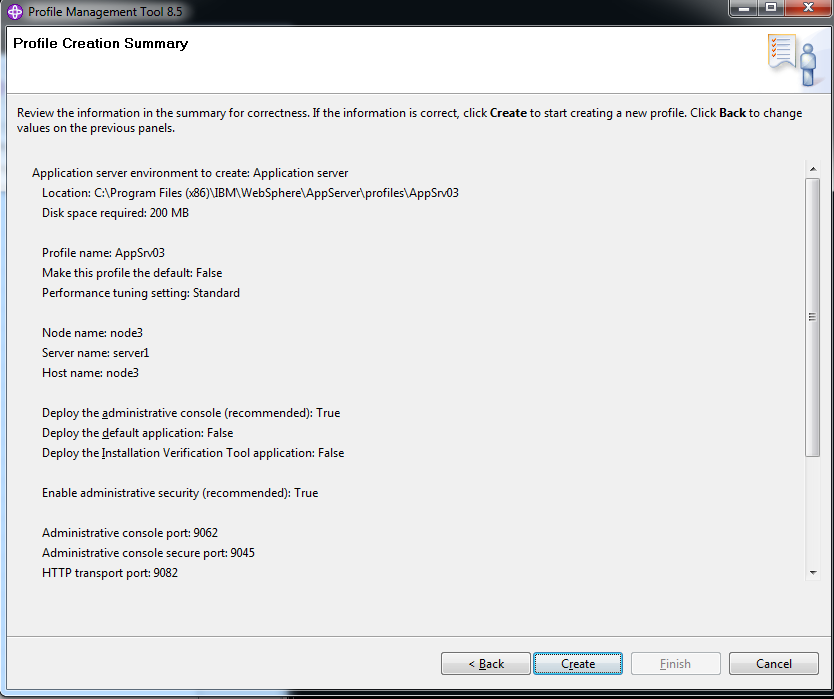
\includegraphics{./images/websphere-02-profile.png}
\caption{Example of the settings before creating the profile.}
\end{figure}

\subsubsection{Configuring the WebSphere Application
Server}\label{configuring-the-websphere-application-server}

In this version of WebSphere, servlet filters are not initialized on web
application startup, but rather, on first access. This can cause
problems when deploying certain apps to Liferay DXP. To configure
servlet filters to initialize on application startup (i.e., deployment),
set the following \texttt{webcontainer} properties in your WebSphere
application server:

\begin{verbatim}
com.ibm.ws.webcontainer.initFilterBeforeInitServlet = true
com.ibm.ws.webcontainer.invokeFilterInitAtStartup = true
\end{verbatim}

To set \texttt{webcontainer} properties in the WebSphere application
server, follow the instructions
\href{http://www-01.ibm.com/support/docview.wss?rss=180&uid=swg21284395}{here
in WebSphere's documentation}.

\subsubsection{Setting up JVM Parameters for Liferay
DXP}\label{setting-up-jvm-parameters-for-liferay-dxp}

Next, in the WebSphere profile you created for Liferay DXP, you must set
an argument that supports Liferay DXP's Java memory requirements. You'll
modify this file:

\begin{verbatim}
[Install Location]/WebSphere/AppServer/profiles/your-profile/config/cells/your-cell/nodes/your-node/servers/your-server/server.xml
\end{verbatim}

Add \texttt{maximumHeapSize="2048"} inside the \texttt{jvmEntries} tag.
For example:

\begin{verbatim}
<jvmEntries xmi:id="JavaVirtualMachine_1183122130078" ... maximumHeapSize="2048">
\end{verbatim}

\noindent\hrulefill

\textbf{Note:} The JVM parameters used here are defaults intended for
initial deployment of production systems. Administrators should change
the settings to values that best address their specific environments.
These must be tuned depending on need.

\noindent\hrulefill

Administrators can set the UTF-8 properties in the \texttt{server.xml}
file. This is required or else special characters will not be parsed
correctly. Add the following inside the \texttt{jvmEntries} tag:

\begin{verbatim}
<jvmEntries xmi:id="JavaVirtualMachine_1183122130078" ...genericJvmArguments="-Dfile.encoding=UTF-8 -Duser.timezone=GMT">
\end{verbatim}

\noindent\hrulefill

\textbf{Important:} For Liferay DXP to work properly, the application
server JVM must use the \texttt{GMT} time zone and \texttt{UTF-8} file
encoding.

\noindent\hrulefill

Alternately, you can set the UTF-8 properties from the WebSphere Admin
Console. (See below.)

\noindent\hrulefill

\textbf{Important:} On JDK 11, the setting
\texttt{-Djava.locale.providers=JRE,COMPAT,CLDR} is required to display
four-digit years. Since JDK 9, the Unicode Common Locale Data Repository
(CLDR) is the default locales provider. CLDR does not provide years in a
four-digit format (see
\href{https://issues.liferay.com/browse/LPS-87191}{LPS-87191}). This
setting works around the issue by using JDK 8's default locales
provider.

\noindent\hrulefill

\subsubsection{Removing the secureSessionCookie
Tag}\label{removing-the-securesessioncookie-tag}

In the same profile, you should delete a problematic
\texttt{secureSessionCookie} tag that can cause Liferay DXP startup
errors. Note that this is just a default setting; once Liferay DXP is
installed, you should tune it appropriately based on your usage.

In
\texttt{{[}Install\ Location{]}/WebSphere/AppServer/profiles/your-profile/config/cells/your-cell/cell.xml},
Delete the \texttt{secureSessionCookie} tag containing
\texttt{xmi:id="SecureSessionCookie\_1"}.

If this tag is not removed, an error similar to this may occur:

\begin{verbatim}
WSVR0501E: Error creating component com.ibm.ws.runtime.component.CompositionUnitMgrImpl@d74fa901    
com.ibm.ws.exception.RuntimeWarning: com.ibm.ws.webcontainer.exception.WebAppNotLoadedException: Failed to load webapp: Failed to load webapp: SRVE8111E: The application, LiferayEAR, is trying to modify a cookie which matches a pattern in the restricted programmatic session cookies list [domain=*, name=JSESSIONID, path=/].
\end{verbatim}

\subsection{Installing Liferay DXP's
Dependencies}\label{installing-liferay-dxps-dependencies}

You must now install Liferay DXP's dependencies. Recall that earlier you
downloaded two ZIP files containing these dependencies. Install their
contents now:

\begin{enumerate}
\def\labelenumi{\arabic{enumi}.}
\item
  \texttt{liferay-dxp-dependencies-{[}version{]}.zip}: Unzip this file
  and place its contents in your WebSphere application server's
  \texttt{{[}Install\ \ \ \ \ Location{]}/WebSphere/AppServer/lib/ext}
  folder. If you have a JDBC database driver \texttt{JAR}, copy it to
  this location as well.
\item
  \texttt{liferay-dxp-osgi-{[}version{]}.zip}: Unzip this file and place
  its contents in the \texttt{{[}Liferay\ Home{]}/osgi} folder (create
  this folder if it doesn't exist). This is typically
  \texttt{{[}Install\ \ \ \ \ Location{]}/WebSphere/AppServer/profiles/your-profile/liferay/osgi}.
\end{enumerate}

\subsubsection{Installing the DXP
portlet.jar}\label{installing-the-dxp-portlet.jar}

DXP's \texttt{portlet.jar} (version 3) is backwards-compatible. It is
included with the Dependencies ZIP that you unzipped above. WebSphere
contains an older \texttt{portlet.jar} version which must be overridden.

\begin{enumerate}
\def\labelenumi{\arabic{enumi}.}
\item
  In your
  \texttt{{[}Install\ Location{]}/WebSphere/AppServer/profiles/your-profile/}
  folder, create a folder called \texttt{app\_shared\_libraries}.
\item
  Move DXP's \texttt{portlet.jar} from the
  \texttt{{[}Install\ Location{]}/WebSphere/AppServer/lib/ext} folder to
  the \texttt{app\_shared\_libraries} folder you created.
\item
  Follow IBM's steps for
  \href{https://www.ibm.com/support/pages/best-practice-using-common-application-files\#usingserver}{using
  a server associated shared library}; make sure to choose \emph{Classes
  loaded with local class loader first (parent\_Last)} on step 4d.
\item
  Save the configuration.
\end{enumerate}

\subsubsection{Ensuring That the DXP Portlet.jar is Loaded
First}\label{ensuring-that-the-dxp-portlet.jar-is-loaded-first}

In addition to placing DXP's \texttt{portlet.jar} in a server associated
shared library, configure the \texttt{config.ini} file so that it is
loaded first.

\begin{enumerate}
\def\labelenumi{\arabic{enumi}.}
\tightlist
\item
  Open the
  \texttt{{[}Install\ Location{]}/WebSphere/AppServer/configuration/config.ini}
  file.
\item
  Find the property \texttt{com.ibm.CORBA,com.ibm}.
\item
  Insert the property
  \texttt{javax.portlet,javax.portlet.filter,javax.portlet.annotations}
  after \texttt{com.ibm.CORBA} and before \texttt{com.ibm}.
\item
  Save the file.
\end{enumerate}

Start the server profile you created for Liferay DXP. Once it starts,
you're ready to configure your database.

\subsection{Database Configuration}\label{database-configuration-5}

If you want WebSphere to manage the database connections, follow the
instructions below. Note this is not necessary if you plan to use
Liferay DXP's standard database configuration; in that case, skip this
section. You'll set your database information in Liferay DXP's setup
wizard after the install.

\noindent\hrulefill

\textbf{Note:} Although Liferay DXP's embedded database is fine for
testing purposes, you \textbf{should not} use it for production Liferay
DXP instances.

\noindent\hrulefill

\begin{figure}
\centering
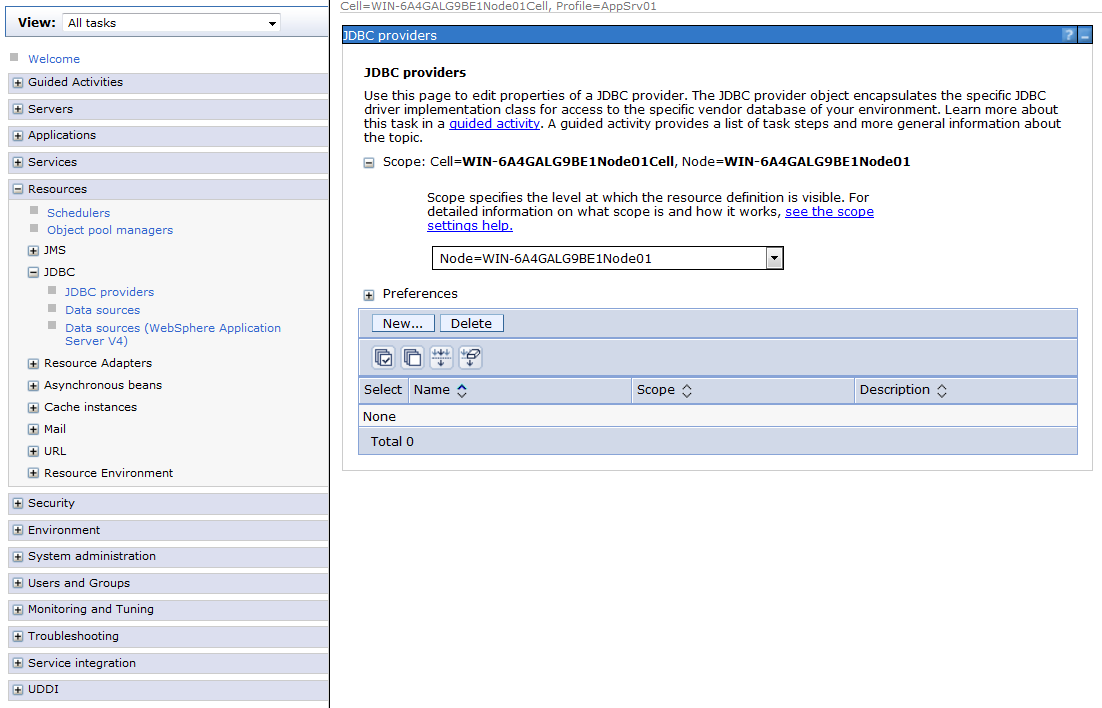
\includegraphics{./images/websphere-jdbc-providers.png}
\caption{WebSphere JDBC providers}
\end{figure}

\begin{enumerate}
\def\labelenumi{\arabic{enumi}.}
\item
  Start WebSphere.
\item
  Open the Administrative Console and log in.
\item
  Click \emph{Resources → JDBC Providers}.
\item
  Select a scope and then click \emph{New}.
\item
  Select your database type, provider type, and implementation type. If
  you select a predefined database, the wizard fills in the name and
  description fields for you. If the database you want to use isn't
  listed, select \emph{User-defined} from the \emph{Database type} field
  and then fill in the \emph{Implementation Class Name}. For example, if
  you use MySQL, select \emph{Database type} → \emph{User-defined}, and
  then enter
  \texttt{com.mysql.jdbc.jdbc2.optional.MysqlConnectionPoolDataSource}
  in \emph{Implementation Class Name}. Click \emph{Next} when you are
  finished.
\item
  Clear any text in the classpath settings. You already copied the
  necessary JARs to a location on the server's classpath. Click
  \emph{Next}.
\item
  Review your settings and click \emph{Finish}. The final configuration
  should look like this:

  \begin{figure}
  \centering
  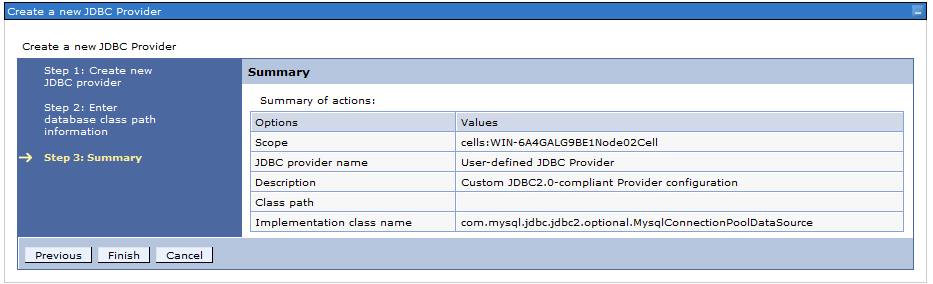
\includegraphics{./images/websphere-03.png}
  \caption{Completed JDBC provider configurations.}
  \end{figure}
\item
  Click your new provider configuration when it appears in the table,
  and then click \emph{Data Sources} under \emph{Additional Properties}.
  Click \emph{New}.
\item
  Enter \emph{liferaydatabasesource} in the \emph{Data source name}
  field and \texttt{jdbc/LiferayPool} in the \emph{JNDI name} field.
  Click \emph{Next}.
\item
  Click \emph{Next} in the remaining screens of the wizard to accept the
  default values. Then review your changes and click \emph{Finish}.
\item
  Click the data source when it appears in the table and then click
  \emph{Custom Properties}. Now click the \emph{Show Filter Function}
  button. This is the second from last of the small icons under the
  \emph{New} and \emph{Delete} buttons.
\item
  Type \emph{user} into the search terms and click \emph{Go}.

  \begin{figure}
  \centering
  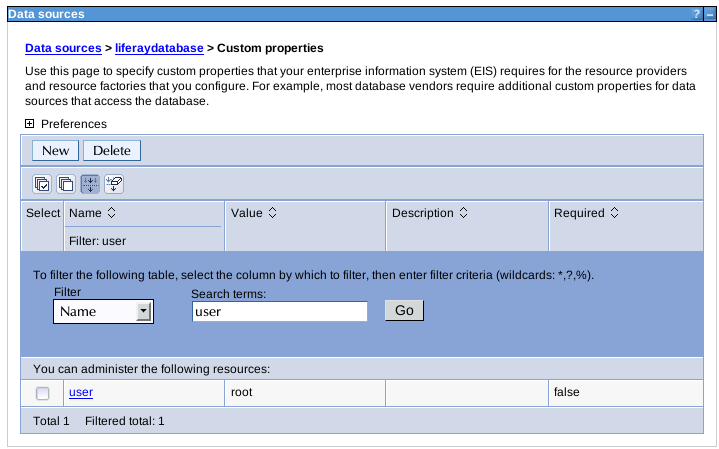
\includegraphics{./images/websphere-database-properties.png}
  \caption{Modifying data source properties in WebSphere}
  \end{figure}
\item
  Select the \emph{user} property and give it the value of the user name
  to your database. Click \emph{OK} and save to master configuration.
\item
  Do another filter search for the \emph{url} property. Give this
  property a value that points to your database. For example, a MySQL
  URL would look like this:

\begin{verbatim}
jdbc:mysql://localhost/lportal?useUnicode=true&characterEncoding=UTF-8&useFastDateParsing=false
\end{verbatim}

  Click \emph{OK} and save to master configuration.
\item
  Do another filter search for the \emph{password} property. Enter the
  password for the user ID you added earlier as the value for this
  property. Click \emph{OK} and save to master configuration.
\item
  Go back to the data source page by clicking it in the breadcrumb
  trail. Click the \emph{Test Connection} button. It should connect
  successfully.
\end{enumerate}

Once you've set up your database, you can set up your mail session.

\subsection{Mail Configuration}\label{mail-configuration-5}

If you want WebSphere to manage your mail sessions, use the following
procedure. If you want to use Liferay DXP's built-in mail sessions, you
can skip this section.

\subsubsection{Creating a WebSphere-Managed Mail Session
(Optional)}\label{creating-a-websphere-managed-mail-session-optional}

\begin{enumerate}
\def\labelenumi{\arabic{enumi}.}
\item
  Click \emph{Resources → Mail → Mail Providers}.
\item
  Click the Built-In Mail Provider for your node and server.
\item
  Click \emph{Mail Sessions} and then click the \emph{New} button.
\item
  Give your mail session a name of \emph{liferaymail} and a JNDI name of
  \texttt{mail/MailSession}. Fill in the correct information for your
  mail server in the sections \emph{Outgoing Mail Properties} and
  \emph{Incoming Mail Properties}. Click \emph{OK} and then save to the
  master configuration.
\item
  Click your mail session when it appears in the table and select
  \emph{Custom Properties} under the \emph{Additional Properties}
  section. Set any other JavaMail properties required by your mail
  server, such as the protocol, ports, whether to use SSL, and so on.
\item
  Click \emph{Security → Global Security} and de-select \emph{Use Java 2
  security to restrict application access to local resources} if it is
  selected. Click \emph{Apply}.
\end{enumerate}

Note that you may also need to retrieve a SSL certificate from your mail
server and add it to WebSphere's trust store. See WebSphere's
documentation for instructions on this.

\subsubsection{Verifying WebSphere Mail
Provider}\label{verifying-websphere-mail-provider}

To validate that the mail session has been configured correctly, there
are a number of ways to test this once the WAR has been deployed, the
server has started, and the user has signed in as the system
administrator. One quick way to validate is to create a new user with a
valid email account. The newly created user should receive an email
notification. The logs should display that the SMTP server has been
pinged with the correct port number listed.

\subsection{Enable Cookies for HTTP
Sessions}\label{enable-cookies-for-http-sessions}

WebSphere restricts cookies to HTTPS sessions by default. If you're
using HTTP instead, this prevents users from signing in to Liferay DXP
and displays the following error in the console:

\begin{verbatim}
20:07:14,021 WARN  [WebContainer : 1][SecurityPortletContainerWrapper:341]
User 0 is not allowed to access URL http://localhost:9081/web/guest/home and
portlet com_liferay_login_web_portlet_LoginPortlet
\end{verbatim}

This occurs because Liferay DXP can't use the HTTPS cookie when you use
HTTP. The end result is that new sessions are created on each page
refresh. Follow these steps to resolve this issue in WebSphere:

\begin{enumerate}
\def\labelenumi{\arabic{enumi}.}
\item
  Click \emph{Application Servers} → \emph{server1} → \emph{Session
  Management} → Enable Cookies
\item
  De-select \emph{Restrict cookies to HTTPS sessions}
\item
  Click \emph{Apply}
\item
  Click \emph{Save}
\end{enumerate}

\subsection{Enable UTF-8}\label{enable-utf-8}

If you did not add the \texttt{-Dfile.encoding=UTF-8} property in the
\texttt{server.xml}, you can do so in the Administrative Console.

\begin{enumerate}
\def\labelenumi{\arabic{enumi}.}
\item
  Click \emph{Application Servers} → \emph{server1} → \emph{Process
  definition}.
\item
  Click \emph{Java Virtual Machine} under \emph{Additional Properties}.
\item
  Enter \texttt{-Dfile.encoding=UTF-8} in the \emph{Generic JVM
  arguments} field.
\item
  Click \emph{Apply} and then \emph{Save} to master configuration.
\end{enumerate}

Once the changes have been saved, Liferay DXP can parse special
characters if there is localized content.

\subsection{Deploy Liferay DXP}\label{deploy-liferay-dxp}

Now you're ready to deploy Liferay DXP!

\begin{enumerate}
\def\labelenumi{\arabic{enumi}.}
\item
  In WebSphere's administrative console, click \emph{Applications} →
  \emph{New Application} → \emph{New Enterprise Application}.
\item
  Browse to the Liferay DXP \texttt{.war} file, select it, and click
  \emph{Next}.
\item
  Leave \emph{Fast Path} selected and click \emph{Next}. Ensure that
  \emph{Distribute Application} has been checked and click \emph{Next}
  again.
\item
  Choose the WebSphere runtimes and/or clusters where you want Liferay
  DXP deployed. Click \emph{Next}.
\item
  Select the virtual host to deploy Liferay DXP on and click
  \emph{Next}.
\item
  Map Liferay DXP to the root context (/) and click \emph{Next}.
\item
  Select the \emph{metadata-complete attribute} setting that you want to
  use and click \emph{Next}.
\item
  Ensure that you have made all the correct choices and click
  \emph{Finish}. When Liferay DXP has installed, click \emph{Save to
  Master Configuration}.

  \begin{figure}
  \centering
  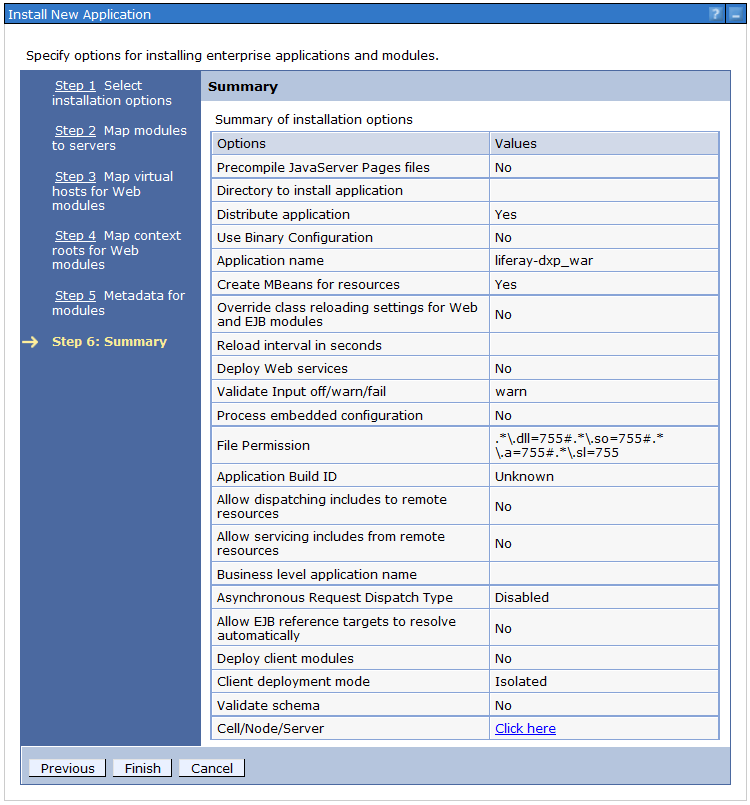
\includegraphics{./images/websphere-deploy-dxp.png}
  \caption{Review your deployment options before deploying.}
  \end{figure}
\end{enumerate}

You've now installed Liferay DXP!

\subsection{Setting the JDK Version for Compiling
JSPs}\label{setting-the-jdk-version-for-compiling-jsps}

Liferay DXP requires that its JSPs are compiled to the Java 8 bytecode
format. To ensure that WebSphere does this, shut down WebSphere after
you've deployed the Liferay DXP \texttt{.war} file. Navigate to the
\texttt{WEB\_INF} folder and add the following setting to the
\texttt{ibm-web-ext.xml} or in most cases the \texttt{ibm-web-ext.xmi}
file:

\begin{verbatim}
<jsp-attribute name="jdkSourceLevel" value="18" />
\end{verbatim}

The exact path to the \texttt{ibm-web-ext.xmi} file depends on your
WebSphere installation location and Liferay DXP version, but here's an
example:

\begin{verbatim}
/opt/IBM/WebSphere/AppServer/profiles/AppSrv01/config/cells/localhostNode01Cell/applications/liferayXX.ear/deployments/liferayXX/liferayXX.war/WEB-INF/ibm-web-ext.xmi
\end{verbatim}

Note that the Liferay DXP \texttt{.war} comes pre-packaged with the
\texttt{ibm-web-ext.xmi} file; this format is functionally the same as
\texttt{.xml} and WebSphere recognizes both formats. For more general
information on how WebSphere compiles JSPs see IBM's official
documentation for
\href{https://www.ibm.com/support/knowledgecenter/en/SSAW57_8.5.5/com.ibm.websphere.nd.doc/ae/rweb_jspengine.html}{WebSphere
Application Server 8.5.5.x} or
\href{https://www.ibm.com/support/knowledgecenter/en/SSEQTP_9.0.0/com.ibm.websphere.base.doc/ae/rweb_jspengine.html}{WebSphere
Application Server 9.0.0.x}.

Now restart WebSphere.

\subsection{Start Liferay DXP}\label{start-liferay-dxp}

\begin{enumerate}
\def\labelenumi{\arabic{enumi}.}
\item
  If you plan to use Liferay DXP's setup wizard, skip to the next step.
  If you wish to use WebSphere's data source and mail session, create a
  file called \texttt{portal-ext.properties} in your Liferay Home
  folder. Place the following configuration in the file:

\begin{verbatim}
 jdbc.default.jndi.name=jdbc/LiferayPool
 mail.session.jndi.name=mail/MailSession
 setup.wizard.enabled=false
\end{verbatim}
\item
  In the WebSphere administrative console, navigate to \emph{Enterprise
  Applications}, select the Liferay DXP application, and click
  \emph{Start}. While Liferay DXP is starting, WebSphere displays a
  spinning graphic. Don't watch it too closely, or you might get
  hypnotized.
\item
  In Liferay DXP's setup wizard, select and configure your database
  type. Click \emph{Finish} when you're done. Liferay DXP then creates
  the tables it needs in the database.
\end{enumerate}

Congratulations! You've installed Liferay DXP on WebSphere!

\noindent\hrulefill

After deploying Liferay DXP, you may see excessive warnings and log
messages, such as the ones below, involving \texttt{PhaseOptimizer}.
These are benign and can be ignored. Make sure to adjust your app
server's logging level or log filters to avoid excessive benign log
messages.

\begin{verbatim}
 May 02, 2018 9:12:27 PM com.google.javascript.jscomp.PhaseOptimizer$NamedPass process
 WARNING: Skipping pass gatherExternProperties
 May 02, 2018 9:12:27 PM com.google.javascript.jscomp.PhaseOptimizer$NamedPass process
 WARNING: Skipping pass checkControlFlow
 May 02, 2018 9:12:27 PM com.google.javascript.jscomp.PhaseOptimizer$NamedPass process
 INFO: pass supports: [ES3 keywords as identifiers, getters, reserved words as properties, setters, string continuation, trailing comma, array pattern rest, arrow function, binary literal, block-scoped function declaration, class, computed property, const declaration, default parameter, destructuring, extended object literal, for-of loop, generator, let declaration, member declaration, new.target, octal literal, RegExp flag 'u', RegExp flag 'y', rest parameter, spread expression, super, template literal, modules, exponent operator (**), async function, trailing comma in param list]
 current AST contains: [ES3 keywords as identifiers, getters, reserved words as properties, setters, string continuation, trailing comma, array pattern rest, arrow function, binary literal, block-scoped function declaration, class, computed property, const declaration, default parameter, destructuring, extended object literal, for-of loop, generator, let declaration, member declaration, new.target, octal literal, RegExp flag 'u', RegExp flag 'y', rest parameter, spread expression, super, template literal, exponent operator (**), async function, trailing comma in param list, object literals with spread, object pattern rest]
\end{verbatim}

\section{Installing Elasticsearch}\label{installing-elasticsearch}

Liferay DXP uses Elasticsearch to index its content. By default, it's
installed as an embedded service. It works, but it's not a supported
configuration for a production server. Feel free to use it while testing
or developing, but when you're ready to put your site in production, you
must run Elasticsearch as a standalone process. This is better anyway,
because it frees you to design your infrastructure the way you want it.
If you've got hardware or a VM to spare, you can separate your search
infrastructure from Liferay DXP and reap some performance gains by
putting search on a separate box. If you're more budget-conscious, you
can still increase performance by running Elasticsearch in a separate,
individually tunable JVM on the same box.

Before installing Elasticsearch, refer to
\href{/docs/7-1/deploy/-/knowledge_base/d/preparing-to-install-elasticsearch}{Preparing
to Install Elasticsearch} for guidance on configuring the servers to
support an Elasticsearch deployment properly.

Installing Elasticsearch is pretty easy and takes only six steps:

\begin{enumerate}
\def\labelenumi{\arabic{enumi}.}
\item
  Find the latest
  \href{https://help.liferay.com/hc/en-us/articles/360016511651\#Liferay-DXP-7.1}{compatible
  version of Elasticsearch}, and then download that version from
  \href{https://www.elastic.co}{Elastic's} website.
\item
  Install Elasticsearch by extracting its archive to the system where
  you want it to run.
\item
  Install some required Elasticsearch plugins.
\item
  Name your Elasticsearch cluster.
\item
  Configure Liferay DXP to connect to your Elasticsearch cluster.
\end{enumerate}

\noindent\hrulefill

\begin{verbatim}
**Note:** If you are installing an Elasticsearch version that requires
installation of a new connector application, you must disable several
version-specific modules. The instructions in [Installing Elasticsearch
7](/docs/7-1/deploy/-/knowledge_base/d/installing-elasticsearch-7)
demonstrate this.
\end{verbatim}

\noindent\hrulefill

\begin{enumerate}
\def\labelenumi{\arabic{enumi}.}
\setcounter{enumi}{5}
\tightlist
\item
  Restart Liferay DXP and reindex your search indexes.
\end{enumerate}

\noindent\hrulefill

\textbf{Note:} Before continuing, make sure you have set the
\href{https://docs.oracle.com/cd/E19182-01/820-7851/inst_cli_jdk_javahome_t/}{\texttt{JAVA\_HOME}
environment variable}.

If you have multiple JDKs installed, make sure Elasticsearch and Liferay
DXP are using the same version and distribution (e.g., Oracle Open JDK
1.8.0\_201). You can specify this in
\texttt{{[}Elasticsearch\ Home{]}/bin/elasticsearch.in.sh}:

\begin{verbatim}
     JAVA_HOME=/path/to/java
\end{verbatim}

Consult the
\href{https://www.elastic.co/support/matrix\#matrix_jvm}{Elasticsearch
compatibility matrix} and the
\href{https://help.liferay.com/hc/en-us/articles/360016285432-Liferay-DXP-7-1-Compatibility-Matrix}{Liferay
DXP compatibility matrix} to learn more about supported JDK
distributions and versions.

\noindent\hrulefill

Now you'll perform these steps, and when you're done, you'll have a
production-ready instance of Liferay DXP up and running.

After you're done following the installation guide, refer to the
\href{discover/deployment/-/knowledge_base/7-1/configuring-elasticsearch-for-liferay-0}{Configuring
Elasticsearch} article for more details on configuring Liferay DXP for
Elasticsearch. For more information on installing a search engine, see
\href{discover/deployment/-/knowledge_base/7-1/installing-a-search-engine}{here}.

\subsubsection{Step One: Find the Right Version of
Elasticsearch}\label{step-one-find-the-right-version-of-elasticsearch}

To install the latest compatible Elasticsearch version, refer to the
\href{https://help.liferay.com/hc/en-us/articles/360016511651\#Liferay-DXP-7.1}{Search
Engine Compatibility Matrix}, and then download that version from
\href{https://www.elastic.co}{Elastic's} website.

To inspect the version of the embedded Elasticsearrch server, if Liferay
DXP isn't running, start it.

Visit port 9200 on localhost to access the embedded Elasticsearch:

\begin{verbatim}
http://localhost:9200
\end{verbatim}

A JSON document is returned that looks similar to this:

\begin{verbatim}
{
  "name" : "g0m223N",
  "cluster_name" : "LiferayElasticsearchCluster",
  "cluster_uuid" : "Ii6STs04Tg-XzTVV5h7M2Q",
  "version" : {
    "number" : "6.5.1",
    "build_hash" : "af51318",
    "build_date" : "2018-01-26T18:22:55.523Z",
    "build_snapshot" : false,
    "lucene_version" : "7.1.0",
    "minimum_wire_compatibility_version" : "5.6.0",
    "minimum_index_compatibility_version" : "5.0.0"
  },
  "tagline" : "You Know, for Search"
}
\end{verbatim}

The version of Elasticsearch that's running is the value of the
\texttt{"number"} field. In this example, it's 6.5.1.

Shut down the Liferay DXP server. In a local, single-machine testing
environment, if you continue without shutting down, the Elasticsearch
server you're about to install and start throws errors in the log if its
cluster name and HTTP port match the already-running embedded
Elasticsearch server. An alternative to shutting down Liferay DXP is to
use a different cluster name (i.e., not
\texttt{LiferayElasticsearchCluster}) and HTTP port (i.e., not
\texttt{9200}) in the remote Elasticsearch server.

Now that you know the version of Elasticsearch you need, go to
\href{https://www.elastic.co}{Elastic's} website and download that
version.

\subsubsection{Step Two: Install
Elasticsearch}\label{step-two-install-elasticsearch}

Most of this step entails deciding where you want to run Elasticsearch.
Do you want to run it on the same machine as Liferay DXP, or do you want
to run it on its own hardware? The answer to this question comes down to
a combination of the resources you have available and the size of your
installation. Regardless of what you decide, either way you get the
benefit of a separately tunable search infrastructure.

Once you have a copy of the right version of Elasticsearch, extract it
to a folder on the machine where you want it running. That's it!

\subsubsection{Step Three: Install Elasticsearch
Plugins}\label{step-three-install-elasticsearch-plugins}

Install the following required Elasticsearch plugins:

\begin{itemize}
\tightlist
\item
  \texttt{analysis-icu}
\item
  \texttt{analysis-kuromoji}
\item
  \texttt{analysis-smartcn}
\item
  \texttt{analysis-stempel}
\end{itemize}

To install these plugins, navigate to Elasticsearch Home and enter

\begin{verbatim}
./bin/elasticsearch-plugin install [plugin-name]
\end{verbatim}

Replace \emph{{[}plugin-name{]}} with the Elasticsearch plugin's name.

\subsubsection{Step Four: Name Your Elasticsearch
Cluster}\label{step-four-name-your-elasticsearch-cluster}

A \emph{cluster} in Elasticsearch is a collection of nodes (servers)
identified as a cluster by a shared cluster name. The nodes work
together to share data and workload. A one node cluster is discussed
here; to create a multi-node cluster, please refer to
\href{https://www.elastic.co/guide/index.html}{Elastic's documentation}.

Now that you've installed Elastic, it sits in a folder on your machine,
which is referred to here as \texttt{{[}Elasticsearch\ Home{]}}. To name
your cluster, you'll define the cluster name in both Elasticsearch and
in Liferay DXP. First, define it in Elasticsearch. Edit the following
file:

\begin{verbatim}
[Elasticsearch Home]/config/elasticsearch.yml
\end{verbatim}

Uncomment the line that begins with \texttt{cluster.name}. Set the
cluster name to whatever you want to name your cluster:

\begin{verbatim}
cluster.name: LiferayElasticsearchCluster
\end{verbatim}

Of course, this isn't a very imaginative name; you may choose to name
your cluster \texttt{finders\_keepers} or something else you can
remember more easily. Save the file.

Now you can start Elasticsearch. Run the executable for your operating
system from the \texttt{{[}Elasticsearch\ Home{]}/bin} folder:

\begin{verbatim}
./elasticsearch
\end{verbatim}

Elasticsearch starts, and one of its status messages includes a
transport address:

\begin{verbatim}
[2018-04-03T15:34:19,784][INFO ][o.e.t.TransportService   ] [g0m223N] publish_address {127.0.0.1:9300}, bound_addresses {[::1]:9300}, {127.0.0.1:9300}
\end{verbatim}

Take note of this address; you'll need to give it to your Liferay DXP
server so it can find Elasticsearch on the network.

\subsubsection{Step Five: Configure Liferay DXP to Connect to your
Elasticsearch
Cluster}\label{step-five-configure-liferay-dxp-to-connect-to-your-elasticsearch-cluster}

Now that you're ready to configure Liferay DXP, start it if you haven't
already, log in, and then click on \emph{Control Panel} →
\emph{Configuration} → \emph{System Settings} → \emph{Search}. Enter the
term \emph{elasticsearch} in the search bar and click the
\emph{Elasticsearch 6} entry from the list of settings. Now you can
configure it. Here are the configuration options to change:

\textbf{Cluster Name:} Enter the name of the cluster as you defined it
in Elasticsearch.

\textbf{Operation Mode:} Defaults to EMBEDDED. Change it to REMOTE to
connect to a standalone Elasticsearch.

\textbf{Transport Addresses:} Enter a delimited list of transport
addresses for Elasticsearch nodes. Here, you'll enter the transport
address from the Elasticsearch server you started. The default value is
\texttt{localhost:9300}, which will work.

When finished, click \emph{Save}. You're almost done.

\subsubsection{Step Six: Restart Liferay DXP and
Reindex}\label{step-six-restart-liferay-dxp-and-reindex}

Stop and restart Liferay DXP. When it's back up, log in as an
administrative user and click on \emph{Control Panel} →
\emph{Configuration} → \emph{Search} and click the \emph{Execute} button
for \emph{Reindex all search indexes}. When you do that, you should see
some messages scroll up in the Elasticsearch log.

For more details refer to the
\href{https://www.elastic.co/guide/en/elasticsearch/reference/6.x/getting-started-install.html}{Elasticsearch
installation guide}.

\section{Trial Plugin Installation}\label{trial-plugin-installation}

For Liferay customers who are evaluating Liferay DXP on a trial basis,
\textbf{the plugins can be accessed from within the \emph{Apps} →
\emph{Store} (i.e., Marketplace) section of the Control Panel in your
product installation}.

\subsection{Installation Process}\label{installation-process}

Follow the steps below to install a trial plugin:

\begin{enumerate}
\def\labelenumi{\arabic{enumi}.}
\item
  Register a \texttt{liferay.com} account (LRDC) account by visiting
  Liferay's home page (if necessary). Do this by clicking \emph{Sign
  In/Create Account} button from the top right Profile button.

  \begin{figure}
  \centering
  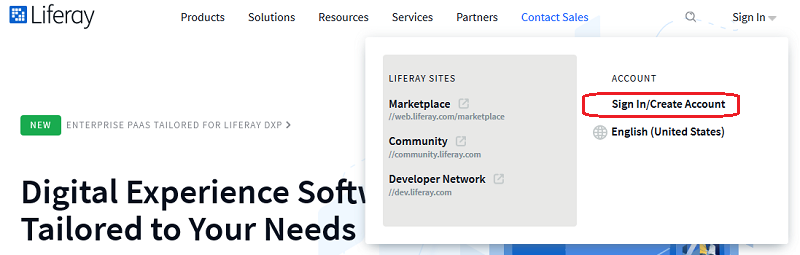
\includegraphics{./images/liferay-com-sign-in.png}
  \caption{Hover over the Profile button and click \emph{Sign In/Create
  Account}.}
  \end{figure}
\item
  Start your Liferay DXP instance (trial license is OK).
\item
  After signing in as an Admin in your Liferay DXP trial server, go to
  the Control Panel → \emph{Apps} → \emph{Store} and configure the
  \texttt{liferay.com} (LRDC) account to log in to the Marketplace.
  Authorize Marketplace to access your local account.

  \begin{figure}
  \centering
  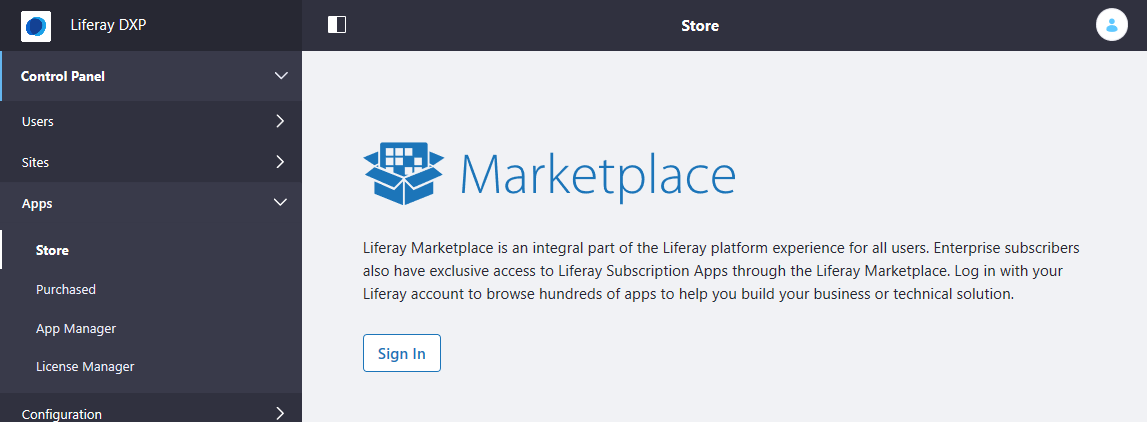
\includegraphics{./images/dxp-store-link.png}
  \caption{Click the \emph{Store} link and authorize Marketplace to
  access your local account.}
  \end{figure}
\item
  Once signed into the Store, click on the \emph{Purchased} link, and
  then click on the \emph{EE} subtab.

  \begin{figure}
  \centering
  \includegraphics{./images/dxp-store-ee.png}
  \caption{The trial plugins are available as plugins already
  purchased.}
  \end{figure}

  Here you can see a list of Liferay DXP plugins that are installed, as
  well as options to update or install certain plugins. To install a
  plugin, click the \emph{Install} button located to the far right of
  the respective plugin. Similarly, click the \emph{Update} button to
  update a plugin.
\end{enumerate}

\noindent\hrulefill

\textbf{Note:} At a later date, the Marketplace website on
\texttt{liferay.com} will be accessible to Liferay DXP trial customers.
For now, please access subscription apps through the portal installation
itself.

\noindent\hrulefill

\subsection{FAQ}\label{faq}

\textbf{Q:} Where are the \emph{Liferay DXP Trial Plugins}?

\textbf{A:} There is no such thing. The Liferay DXP plugins in Liferay
Marketplace are the same ones that you get to try out with your Liferay
DXP trial license for your portal. The Liferay DXP license (trial or
official Liferay DXP subscriber) gives you access to the Liferay DXP
plugins. Also, there is no difference code-wise or release-wise between
a Liferay DXP trial installation and a regular Liferay DXP non-trial
installation. The only difference is the license.

\textbf{Q:} Why can't I go to liferay.com/marketplace? Why can't I
\emph{purchase} from the Marketplace site?

\textbf{A:} DXP trial users must use the Marketplace from within the
product's Control Panel (instructions above). You do not need to
\emph{purchase} any DXP plugins because if you access Marketplace from
within the Control Panel, Marketplace sees that you have a DXP license
installed and gives access to DXP plugins. Official DXP subscription
customers (i.e., non trial) can log into \texttt{liferay.com} with their
designated DXP subscriber login and access all DXP plugins through the
Marketplace website.

\textbf{Q:} Why are the plugins under the Purchased tab? If I click on
the \emph{DXP Marketplace} link, it does not let me get the DXP plugins.

\textbf{A:} Once you're signed into the Store, click on the
\emph{Purchased} tab, then click on the \emph{EE} subtab.

\textbf{Q:} What happens when DXP trial customers become official
Liferay Digital Experience subscribers?

\textbf{A:} They can still complete the above process, or they can also
visit the \href{https://www.liferay.com/marketplace}{Liferay Marketplace
website}.

\textbf{Q:} Do DXP trial customers get the DXP source code?

\textbf{A:} No, they can only install the plugin. The DXP source code
becomes available once they are official Liferay DXP Enterprise
subscribers.

\textbf{Q:} Can this process of installing DXP plugins be used from
Liferay Portal CE (Community Edition)?

\textbf{A:} No, the Marketplace must detect that you are running Liferay
DXP.

\section{Activating Liferay DXP}\label{activating-liferay-dxp}

There are two ways to activate your Liferay DXP instance:

\begin{itemize}
\item
  With an XML activation key that you request and receive from Liferay
  Support.
\item
  Online activation through Liferay Connected Services (LCS). Liferay
  DXP 7.0 introduced LCS as a way to activate Liferay DXP instances. LCS
  can also install fix packs, monitor each instance's performance, and
  help administrators automatically manage Liferay DXP subscriptions.
  See the
  \href{/docs/7-1/deploy/-/knowledge_base/d/managing-liferay-dxp-with-liferay-connected-services}{LCS
  documentation} for instructions on activating your instances with LCS.
\end{itemize}

\noindent\hrulefill

\textbf{Note:} You must use LCS for activation of Elastic subscriptions.
Otherwise, you don't have to use LCS for activation. You can instead
request an XML activation key from Liferay Support.

\noindent\hrulefill

\section{Setting Up Marketplace}\label{setting-up-marketplace}

\href{https://www.liferay.com/marketplace}{Liferay Marketplace} is more
than just a store for Liferay applications. Under the hood, it provides
both the store and Liferay DXP's application deployment features. For
this reason, you must ensure that Marketplace can run and configure
itself.

Here are some scenarios to work around to ensure Marketplace works
successfully:

\begin{itemize}
\tightlist
\item
  \hyperref[server-is-firewalled-without-access-to-the-internet]{Server
  is Firewalled without Access to the Internet}
\item
  \hyperref[limited-database-access]{Limited Database Access}
\end{itemize}

The firewall scenario is discussed first.

\subsection{Server is Firewalled without Access to the
Internet}\label{server-is-firewalled-without-access-to-the-internet}

Your server might be behind a firewall that prevents access to the
Internet. Or your security policy might not allow direct download and
installation from the Internet. In these cases, you have two options:

\begin{enumerate}
\def\labelenumi{\arabic{enumi}.}
\item
  From an Internet-enabled computer, download the
  \href{https://www.liferay.com/marketplace/download}{Marketplace
  plugin}. Then allow Liferay DXP to auto deploy it by dropping the
  downloaded \texttt{.lpkg} file into the \texttt{deploy} folder in
  \href{/docs/7-1/deploy/-/knowledge_base/d/installing-liferay\#liferay-home}{Liferay
  Home}.
\item
  Alternately, once you have the downloaded \texttt{.lpkg} file, deploy
  it using the
  \href{/docs/7-1/user/-/knowledge_base/u/managing-and-configuring-apps}{App
  Manager}.
\end{enumerate}

Next you'll learn how to work around database access restrictions.

\subsection{Limited Database Access}\label{limited-database-access}

Some production environments do not have the necessary database
permissions for Liferay DXP, apps, modules, and plugins to maintain
their tables. In these cases:

\begin{enumerate}
\def\labelenumi{\arabic{enumi}.}
\item
  Grant the Liferay DXP database user temporary full rights to the
  database.
\item
  Install Liferay DXP and start it so that it populates its database.
\item
  Once the database is created, remove the permissions for creating
  tables and dropping tables from the Liferay DXP database user.
\end{enumerate}

See the
\href{/docs/7-1/deploy/-/knowledge_base/d/preparing-for-install\#step-1-choose-a-database-server-and-create-a-new-database}{database
server and new database instructions} for more information. Note that
many sophisticated Liferay DXP apps---not just the Marketplace
app---require new tables when deployed. If your environment restricts
database access, you may need to repeat the above steps whenever you
deploy a new app.

You've prepared Liferay DXP for installing Marketplace and additional
apps.

\chapter{Installing a Search Engine}\label{installing-a-search-engine}

A search engine is a critical component of your Liferay DXP
installation. If you're here, you probably know the basics already and
want to configure a search engine for your Liferay DXP deployment.

Liferay DXP ships with Elasticsearch, a highly scalable, full-text
search engine. Elasticsearch is well-supported and almost certainly
meets any search and indexing need you have. For deployment settings,
learn to configure a standalone or remote Elasticsearch server or
cluster
\href{/docs/7-1/deploy/-/knowledge_base/d/installing-elasticsearch}{here}.

\href{http://lucene.apache.org/solr}{Solr} is also supported in Liferay
DXP.

\section{Choosing a Search Engine}\label{choosing-a-search-engine}

Elasticsearch and Solr are both supported, but there are some
differences in how they work with Liferay DXP. In certain cases, you
must choose Elasticsearch.

If you answer \emph{yes} to either of these questions, you must choose
Elasticsearch:

\begin{enumerate}
\def\labelenumi{\arabic{enumi}.}
\item
  You're using
  \href{/web/commerce/documentation/-/knowledge_base/1-0/getting-started}{Liferay
  Commerce, Liferay's commerce solution}.
\item
  Your custom search code requires the use of the
  \texttt{TermsSetFilter} API or the Geolocation APIs that are
  implemented in the Liferay Connector to Elasticsearch.
\end{enumerate}

@commerce@ requires the \texttt{TermsSetFilter} implementation available
in the Elasticsearch connector, so you must use Elasticsearch if you're
using @commerce@.

Both of these Elasticsearch-only developer features are not currently
implemented in the Liferay Connector to Solr, but may be added in the
future. If you must use either of those features in your search
solution's code, use Elasticsearch. If you're using Liferay Commerce,
use Elasticsearch. Otherwise, feel free to use Elasticsearch or Solr to
index your portal content.

Another factor to consider in your search engine selection is JDK
version. The search engine and Liferay DXP must use the same JDK version
and distribution (e.g., Oracle Open JDK 1.8.0\_201). Consult the
\href{https://www.elastic.co/support/matrix\#matrix_jvm}{Elasticsearch
compatibility matrix} and the
\href{https://help.liferay.com/hc/en-us/articles/360016285432-Liferay-DXP-7-1-Compatibility-Matrix}{Liferay
DXP compatibility matrix} to learn more about supported JDK
distributions and versions. This consideration is not necessary for
Solr, because no JVM level serialization happens between the servers.
All communication occurs at the HTTP level.

\chapter{Elasticsearch}\label{elasticsearch}

Elasticsearch is an open source, highly scalable, full-text search and
analytics engine.

By default, Elasticsearch runs as an embedded search engine, which is
useful for development and testing but is not supported in production.
In production environments you must run Elasticsearch in remote mode, as
a separate server or cluster. This guide walks you through the process
of configuring Elasticsearch in remote mode.

If you'd rather use Solr, it's also supported. See the documentation on
\href{discover/deployment/-/knowledge_base/7-1/installing-solr}{Installing
Solr} if you're interested.

To get up and running quickly with Elasticsearch as a remote server,
refer to the
\href{/docs/7-1/deploy/-/knowledge_base/d/installing-elasticsearch}{Installing
Elasticsearch article}. Those are basic instructions for installing and
configuring Elasticsearch in a single server environment. This article
includes more details and information on clustering and tuning
Elasticsearch. Here, you'll learn to configure your existing
Elasticsearch installation for use in production environments.

If you've come here looking for information on search engines in
general, or the low level search infrastructure of Liferay DXP, refer
instead to the developer tutorial Introduction to Liferay Search (not
yet written).

These terms are useful to understand as you read this guide:

\begin{itemize}
\item
  \emph{Elasticsearch Home} refers to the root folder of your unzipped
  Elasticsearch installation (for example,
  \texttt{elasticsearch-6.5.1}).
\item
  \href{/docs/7-1/deploy/-/knowledge_base/d/installing-liferay\#liferay-home}{\emph{Liferay
  Home}} refers to the root folder of your Liferay DXP installation. It
  contains the \texttt{osgi}, \texttt{deploy}, \texttt{data}, and
  \texttt{license} folders, among others.
\end{itemize}

\section{Embedded vs.~Remote Operation
Mode}\label{embedded-vs.-remote-operation-mode}

When you start Liferay DXP, this message is displayed in the log:

\begin{verbatim}
2018-12-10 16:20:32.987 WARN  [Elasticsearch initialization thread][EmbeddedElasticsearchConnection:288] Liferay is configured to use embedded Elasticsearch as its search engine. Do NOT use embedded Elasticsearch in production. Embedded Elasticsearch is useful for development and demonstration purposes. Refer to the documentation for details on the limitations of embedded Elasticsearch. Remote Elasticsearch connections can be configured in the Control Panel.
\end{verbatim}

When you install Liferay DXP, Elasticsearch is already embedded. In
embedded mode, Elasticsearch search runs in the same JVM to make it easy
to test-drive with minimal configuration. Running both servers in the
same process has drawbacks:

\begin{itemize}
\tightlist
\item
  Elasticsearch must use the same JVM options as Liferay DXP.
\item
  Liferay DXP and Elasticsearch compete for resources.
\end{itemize}

\noindent\hrulefill

\textbf{Note:} While it's not a supported production configuration,
installing Kibana to monitor the embedded Elasticsearch server is useful
during development and testing. Just be aware that you must install the
\href{https://www.elastic.co/downloads/kibana-oss}{OSS only Kibana
build}.

\noindent\hrulefill

You wouldn't run an embedded database like HSQL in production, and you
shouldn't run Elasticsearch in embedded mode in production either.
Instead, run Elasticsearch in \emph{remote operation mode}, as a
standalone server or cluster of server nodes.

\section{Troubleshooting
Elasticsearch}\label{troubleshooting-elasticsearch}

Sometimes things don't go as planned. If you've set up Liferay DXP with
Elasticsearch in remote mode, but Liferay DXP can't connect to
Elasticsearch, check these things:

\begin{description}
\tightlist
\item[\textbf{Cluster name:}]
The value of the \texttt{cluster.name} property in Elasticsearch must
match the \texttt{clusterName} property you configured for Liferay's
Elasticsearch adapter.
\item[\textbf{Transport address:}]
The value of the \texttt{transportAddress} property in the Elasticsearch
adapter must match the port where Elasticsearch is running. If Liferay
DXP is running in embedded mode, and you start a standalone
Elasticsearch node or cluster, it detects that port \texttt{9300} is
taken and switches to port \texttt{9301}. If you then set Liferay's
Elasticsearch adapter to remote mode, it continues to look for
Elasticsearch at the default port (\texttt{9300}).
\end{description}

The following articles cover the Liferay Connector to Elasticsearch's
configuration options in more detail.

\section{Preparing to Install
Elasticsearch}\label{preparing-to-install-elasticsearch}

By default, 7.0 and its
\href{/docs/7-1/deploy/-/knowledge_base/d/configuring-elasticsearch-for-liferay-0\#embedded-vs-remote-operation-mode}{embedded
Elasticsearch engine} run in the same JVM. Although this enables
out-of-the-box search, it's only supported for development. For
production use, Elasticsearch must run in a separate JVM. See the
\href{/docs/7-1/deploy/-/knowledge_base/d/installing-elasticsearch}{installation
guide} for information on installing a remote Elasticsearch cluster.

Because search engines benefit heavily from caching, their JVM memory
profiles differ substantially from those of a JVM running Liferay DXP.
Therefore, the two applications should always be kept separate in
production environments.

The following sections provide a synopsis of Elasticsearch
configurations for 7.0. Prior to deployment, we strongly recommend
reading
\href{https://www.elastic.co/guide/en/elasticsearch/guide/current/index.html}{Elastic's
documentation on production deployment}.

\subsection{Sizing Your Deployment}\label{sizing-your-deployment}

When sizing your Elasticsearch deployment, carefully consider CPU,
memory, disk, and network capacity. To scale effectively and avoid using
lots of machines, deploy Elasticsearch on medium to large machines (for
example, machines with two to eight CPUs). Avoid running multiple
Elasticsearch JVMs on the same operating system.

\subsection{CPU}\label{cpu}

We recommend allocating at least eight total CPU cores to the
Elasticsearch engine, assuming only one Elasticsearch JVM is running on
the machine.

\subsection{Memory}\label{memory}

At least 16 GB of memory is recommended, with 64 GB preferred. The
precise memory allocation required depends on how much data is indexed.
For index sizes 500 GB to 1 TB, 64 GB of memory suffices.

\subsection{Disk}\label{disk}

Search engines store their indexes on disk, so disk I/O capacity can
impact search performance. Deploy Elasticsearch on SSD whenever
possible. Otherwise use high-performance traditional hard disks (for
example, 15k RPM). In either case, consider using RAID 0.

Avoid using Network Attached Storage (NAS) whenever possible as the
network overhead can be large. If you're using public cloud
infrastructure like Amazon Web Services, use instance local storage
instead of network storage, such as Elastic Block Store (EBS).

Maintain 25 percent more disk capacity than the total size of your
indexes. If your index is 60 GB, make sure you have at least 75 GB of
disk space available. To estimate the disk space you need, you can index
a representative sample of your production content and multiply that
size by the fraction of your production content that it represents. For
example, index 25 percent of your production content and then multiply
the resulting index size by four. Keep in mind that indexing a 1 MB file
doesn't result in 1 MB of disk space in the search index.

\subsection{Cluster Size}\label{cluster-size}

While Liferay DXP can work with an Elasticsearch cluster comprised of
one or two nodes, the minimum cluster size recommended by Elastic for
fault tolerance is three nodes.

\subsection{Networking}\label{networking}

Elasticsearch relies on clustering and sharding to deliver fast,
accurate search results, and thus requires a fast and reliable network.
Most modern data centers provide 1 GbE or 10 GbE between machines.

Elasticsearch doesn't support multi-data center deployments.

\section{Configuring the Liferay Elasticsearch
Connector}\label{configuring-the-liferay-elasticsearch-connector}

For detailed Elasticsearch configuration information, refer to the
\href{https://www.elastic.co/guide/en/elasticsearch/reference/6.5/settings.html}{Elasticsearch
documentation}.

The name of your Elasticsearch cluster is important. When you're running
Elasticsearch in remote mode, the cluster name is used by Liferay DXP to
recognize the Elasticsearch cluster. To learn about setting the
Elasticsearch cluster name on the Liferay DXP side, refer below to the
section called Configuring the Liferay Elasticsearch Connector.

\noindent\hrulefill

\textbf{Note:} The \texttt{http.enabled} setting in Elasticsearch
corresponds to the \texttt{httpEnabled} setting in the Liferay Connector
to Elasticsearch 6 application. As this setting was
\href{https://www.elastic.co/guide/en/elasticsearch/reference/current/release-notes-6.3.0.html\#deprecation-6.3.0}{deprecated
in Elasticsearch 6.3}, the connector's corresponding setting is now also
deprecated. This setting was only used for configuring the embedded
Elasticsearch server, so its deprecation should have minimal impact to
production deployments.

\noindent\hrulefill

Elasticsearch's configuration files are written in
\href{http://www.yaml.org}{YAML} and kept in the
\texttt{{[}Elasticsearch\ Home{]}/config} folder. The main configuration
file is \texttt{elasticsearch.yml}, used for configuring Elasticsearch
modules.

To set the name of the Elasticsearch cluster, open
\texttt{{[}Elasticsearch\ Home{]}/config/elasticsearch.yml} and specify

\begin{verbatim}
cluster.name: LiferayElasticsearchCluster
\end{verbatim}

Since \texttt{LiferayElasticsearchCluster} is the default name given to
the cluster, this would work just fine. Of course, you can name your
cluster whatever you want (we humbly submit the recommendation
\texttt{clustery\_mcclusterface}).\hyperref[footnote1]{1} You can
configure your node name using the same syntax (setting the
\texttt{node.name} property).

If you'd rather work from the command line than in the configuration
file, navigate to Elasticsearch Home and enter

\begin{verbatim}
./bin/elasticsearch --cluster.name clustery_mcclusterface --node.name nody_mcnodeface
\end{verbatim}

Feel free to change the node name or the cluster name. Once you
configure Elasticsearch to your liking, start it up.

\subsection{Starting Elasticsearch}\label{starting-elasticsearch}

Start Elasticsearch by navigating to Elasticsearch Home and typing

\begin{verbatim}
./bin/elasticsearch
\end{verbatim}

if you run Linux, or

\begin{verbatim}
\bin\elasticsearch.bat
\end{verbatim}

if you run Windows.

To run as a daemon in the background, add the \texttt{-d} switch to
either command:

\begin{verbatim}
./bin/elasticsearch -d
\end{verbatim}

Once both Elasticsearch and Liferay DXP are installed and running,
introduce them to each other.

\subsection{Configuring the Liferay Elasticsearch
Connector}\label{configuring-the-liferay-elasticsearch-connector-1}

The Elasticsearch connector provides integration between Elasticsearch
and the portal. Before you configure the connector, make sure
Elasticsearch is running.

There are two ways to configure the adapter:

\begin{enumerate}
\def\labelenumi{\arabic{enumi}.}
\item
  \hyperref[configuring-the-adapter-in-the-control-panel]{Use the System
  Settings application in the Control Panel.}
\item
  \hyperref[configuring-the-adapter-with-an-osgi-config-file]{Manually
  create an OSGi configuration file.}
\end{enumerate}

It's convenient to configure the Elasticsearch adapter from System
Settings, but this is often only possible during development and
testing. If you're not familiar with System Settings, you can read about
it \href{/docs/7-1/user/-/knowledge_base/u/system-settings}{here}.
Remember that you can generate configuration files for deployment to
other systems by configuring System Settings, and then exporting the
\texttt{.config} file with your configuration.

\subsubsection{Configuring the Adapter in the Control
Panel}\label{configuring-the-adapter-in-the-control-panel}

To configure the Elasticsearch adapter from the System Settings
application,

\begin{enumerate}
\def\labelenumi{\arabic{enumi}.}
\item
  Start Liferay DXP.
\item
  Navigate to \emph{Control Panel} → \emph{Configuration} → \emph{System
  Settings} → \emph{Foundation}.
\item
  Find the \emph{Elasticsearch} entry (scroll down and browse to it or
  use the search box) and click the Actions icon
  (
\includegraphics{./images/icon-actions.png}), then \emph{Edit}.

  \begin{figure}
  \centering
  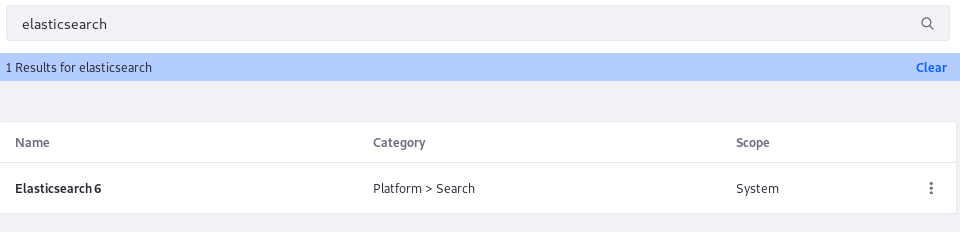
\includegraphics{./images/cfg-elasticsearch-sys-settings.png}
  \caption{Use the System Settings application in Liferay DXP's Control
  Panel to configure the Elasticsearch adapter.}
  \end{figure}
\item
  Make any edits to the configuration and click \emph{Save}.

  \begin{figure}
  \centering
  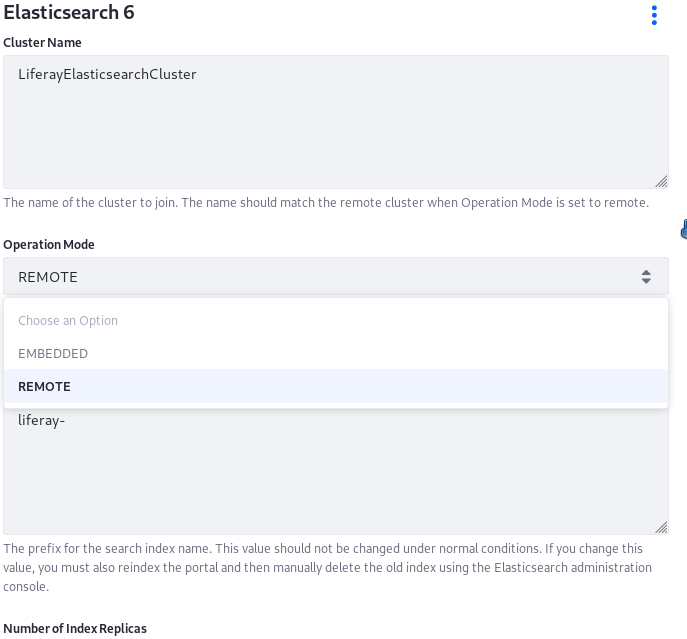
\includegraphics{./images/cfg-elasticsearch-sys-settings2.png}
  \caption{Set configurations for the Elasticsearch connector, like
  settings the Operation Mode to \emph{Remote}.}
  \end{figure}
\end{enumerate}

\noindent\hrulefill

\textbf{Note:} If you switch operation modes (\texttt{EMBEDDED} →
\texttt{REMOTE}), you must trigger a re-index. Navigate to \emph{Control
Panel} → \emph{Configuration} → \emph{Search}, and click \emph{Execute}
next to \emph{Reindex all search indexes.}

\noindent\hrulefill

\subsubsection{\texorpdfstring{Configuring the Adapter with an OSGi
\texttt{.config}
File}{Configuring the Adapter with an OSGi .config File}}\label{configuring-the-adapter-with-an-osgi-.config-file}

When preparing a system for production deployment, you want to use a
repeatable deployment process. Therefore, it's best to use the OSGi
configuration file, where your configuration is maintained in a
controlled source.

Follow these steps to configure the Elasticsearch adapter using a
configuration file:

\begin{enumerate}
\def\labelenumi{\arabic{enumi}.}
\item
  Create the following file:

\begin{verbatim}
 [Liferay_Home]/osgi/configs/com.liferay.portal.search.elasticsearch6.configuration.ElasticsearchConfiguration.config
\end{verbatim}
\item
  Add configurations to the file, in the format
  \texttt{propertyName="Value"}. For example,

\begin{verbatim}
 operationMode="REMOTE"
 # If running Elasticsearch from a different computer:
 #transportAddresses="ip.of.elasticsearch.node:9300"
 # Highly recommended for all non-prodcution usage (e.g., practice, tests, diagnostics):
 #logExceptionsOnly="false"
\end{verbatim}
\item
  Start Liferay DXP or re-index if already running.
\end{enumerate}

As you can see from the System Settings entry for Elasticsearch, there
are a lot more configuration options available that help you tune your
system for optimal performance.

What follows here are some known good configurations for clustering
Elasticsearch. These, however, can't replace the manual process of
tuning, testing under load, and tuning again, so we encourage you to
examine the
\href{https://www.elastic.co/guide/en/elasticsearch/reference/6.5/important-settings.html}{Elasticsearch
documentation} and go through that process once you have a working
configuration.

\subsection{Configuring a Remote Elasticsearch
Host}\label{configuring-a-remote-elasticsearch-host}

In production systems Elasticsearch and Liferay DXP are installed on
different servers. To make Liferay DXP aware of the Elasticsearch
cluster, set

\begin{verbatim}
transportAddresses=[IP address of Elasticsearch Node]:9300
\end{verbatim}

Here's an example that sets the IP address of two nodes in the
Elasticsearch cluster:

\begin{verbatim}
transportAddresses=["192.168.1.1:9300","192.168.1.2:9300"]
\end{verbatim}

Set this in the Elasticsearch connector's OSGi configuration file. List
as many or as few Elasticsearch nodes in this property as you want. This
tells Liferay DXP the IP address or host name where search requests
should be sent. If using System Settings, set the value in the
\emph{Transport Addresses} property.

\noindent\hrulefill

\textbf{Note:} In an Elasticsearch cluster you can list the transport
addresses for multiple Elasticsearch nodes as a comma-separated list in
the \texttt{transportAddresses} property. If you set only one transport
address, Liferay DXP loses contact with Elasticsearch if that node goes
down.

\noindent\hrulefill

On the Elasticsearch side, set the \texttt{network.host} property in
your \texttt{elaticsearch.yml} file. This property simultaneously sets
both the \emph{bind host} (the host where Elasticsearch listens for
requests) and the \emph{publish host} (the host name or IP address
Elasticsearch uses to communicate with other nodes). See
\href{https://www.elastic.co/guide/en/elasticsearch/reference/6.5/modules-network.html}{here}
for more information.

\subsection{Clustering Elasticsearch in Remote Operation
Mode}\label{clustering-elasticsearch-in-remote-operation-mode}

Clustering Elasticsearch is easy. First, set
\texttt{node.max\_local\_storage\_nodes} to be something greater than
\texttt{1}. When you run the Elasticsearch start script, a new local
storage node is added to the cluster. If you want four nodes running
locally, for example, run \texttt{./bin/elasticsearch} four times. See
\href{https://www.elastic.co/guide/en/elasticsearch/reference/6.5/modules-node.html\#max-local-storage-nodes}{here}
for more information.

Configure the number of shards and replicas in the Elasticsearch 6
adapter, using the \texttt{indexNumberOfShards} and
\texttt{indexNumberOfReplicas} properties to specify the number of
primary shards and number of replica shards, respectively.
Elasticsearch's default configuration works for a cluster of up to ten
nodes, since the default number of shards is \texttt{5} and the default
number of replica shards is \texttt{1}.

\noindent\hrulefill

\textbf{Note:} Elasticsearch uses the
\href{https://www.elastic.co/guide/en/elasticsearch/reference/6.5/modules-discovery-zen.html}{Zen
Discovery Module} by default, which provides unicast discovery.
Additionally, nodes in the cluster communicate using the
\href{https://www.elastic.co/guide/en/elasticsearch/reference/6.5/modules-transport.html}{Transport
Module}, through TCP. See the Elasticsearch documentation for the
available properties (to be set in the \texttt{elasticsearch.yml} file),
and the Liferay DXP Elasticsearch Adapter's settings for the adapter's
available settings.

At a minimum, provide the list of hosts (as \texttt{host:port}) to act
as gossip routers during unicast discovery in the
\texttt{elasticsearch.yml}:

\begin{verbatim}
 discovery.zen.ping.unicast.hosts: ["node1.ip.address", "node2.ip.address"]
\end{verbatim}

For example,

\begin{verbatim}
 discovery.zen.ping.unicast.hosts: ["10.10.10.5", "10.10.10,.5:9305"]
\end{verbatim}

\noindent\hrulefill

For more information on configuring an Elasticsearch cluster, see the
documentation on
\href{https://www.elastic.co/guide/en/elasticsearch/guide/current/_index_settings.html}{Elasticsearch
Index Settings}.

\subsection{Elasticsearch Connector System Settings, By Operation
Mode}\label{elasticsearch-connector-system-settings-by-operation-mode}

Some of the settings available for the Elasticsearch connector are
applicable for only one operation mode (REMOTE or EMBEDDED). Refer to
the table below:

Adapter Setting/Operation Mode \textbar{} EMBEDDED \textbar{} REMOTE
\textbar{} \texttt{clusterName} \textbar{} x \textbar{} x
\texttt{operationMode} \textbar{} x \textbar{} x
\texttt{indexNamePrefix} \textbar{} x \textbar{} x
\texttt{indexNumberOfReplicas*} \textbar{} x \textbar{} x
\texttt{indexNumberOfShards*} \textbar{} x \textbar{} x
\texttt{bootstrapMlockAll} \textbar{} x \textbar{} -
\texttt{logExceptionsOnly} \textbar{} x \textbar{} x
\texttt{retryOnConflict} \textbar{} x \textbar{} x
\texttt{discoveryZenPingUnicastHostsPort} \textbar{} x \textbar{} -
\texttt{networkHost} \textbar{} x \textbar{} - \texttt{networkBindHost}
\textbar{} x \textbar{} - \texttt{networkPublishHost} \textbar{} x
\textbar{} - \texttt{transportTcpPort} \textbar{} x \textbar{} -
\texttt{transportAddresses} \textbar{} - \textbar{} x
\texttt{clientTransportSniff} \textbar{} - \textbar{} x
\texttt{clientTransportIgnoreClusterName} \textbar{} - \textbar{} x
\texttt{clientTransportPingTimeout*} \textbar{} - \textbar{} x
\texttt{clientTransportNodesSamplerInterval} \textbar{} - \textbar{} x
\texttt{httpEnabled} \textbar{} x \textbar{} - \texttt{httpCORSEnabled}
\textbar{} x \textbar{} - \texttt{httpCORSAllowOrigin} \textbar{} x
\textbar{} - \texttt{httpCORSConfigurations} \textbar{} x \textbar{} -
\texttt{additionalConfigurations} \textbar{} x \textbar{} x
\texttt{additionalIndexConfigurations} \textbar{} x \textbar{} x
\texttt{additionalTypeMappings} \textbar{} x \textbar{} x
\texttt{overrideTypeMappings} \textbar{} x \textbar{} x
\texttt{syncSearch} \textbar{} x \textbar{} -

* \textbf{Note:} Available in the Connector to Elasticsearch 6 only.

1 This is, of course, a nod to all those fans of
\href{http://www.theatlantic.com/international/archive/2016/05/boaty-mcboatface-parliament-lessons/482046}{Boaty
Mcboatface}.

\section{Advanced Configuration of the Liferay Elasticsearch
Connector}\label{advanced-configuration-of-the-liferay-elasticsearch-connector}

The default configurations for Liferay's Elasticsearch adapter module
are set in a Java class called \texttt{ElasticsearchConfiguration}.

While the Elasticsearch adapter has a lot of configuration options out
of the box, you might find an Elasticsearch configuration you need that
isn't provided by default. In this case, add the configuration options
you need. If something is configurable for Elasticsearch, it's
configurable using the Elasticsearch adapter.

\subsection{Adding Settings and Mappings to the Liferay Elasticsearch
Adapter}\label{adding-settings-and-mappings-to-the-liferay-elasticsearch-adapter}

Think of the available configuration options as being divided into two
groups: the most common ones that are easily configured, and more
complex configurations requiring a more brute-force approach. If a
necessary setting isn't available by default, you can still configure it
with the Liferay Elasticsearch adapter. You'll just need to use one or
more of the \texttt{additionalConfigurations},
\texttt{additionalIndexConfigurations}, or
\texttt{additionalTypeMappings}, and \texttt{overrideTypeMappings}
settings.

\begin{figure}
\centering
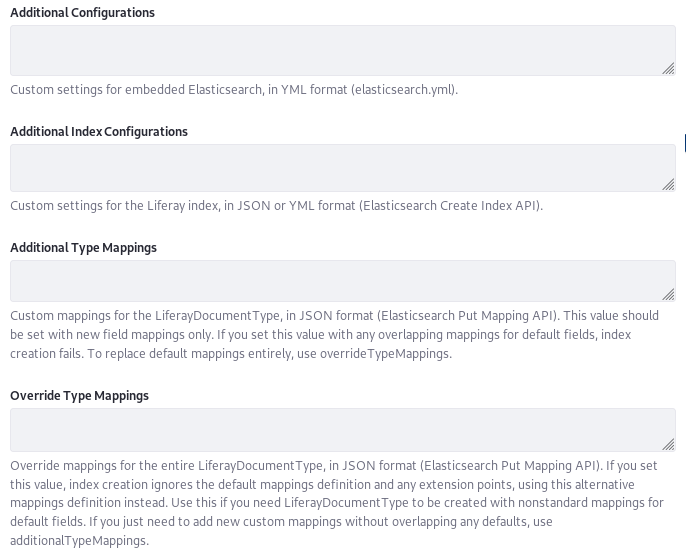
\includegraphics{./images/cfg-elasticsearch-additional-configs.png}
\caption{You can add Elasticsearch configurations to the ones currently
available in System Settings.}
\end{figure}

\subsubsection{Additional
Configurations}\label{additional-configurations}

The \texttt{additionalConfigurations} configuration defines extra
settings (in YAML) for the embedded Elasticsearch. This is only useful
for testing environments using the embedded Elasticsearch server. Any
node settings normally set in \texttt{elasticsearch.yml} can be declared
here. See the
\href{https://www.elastic.co/guide/en/elasticsearch/reference/6.5/index.html}{Elasticsearch
documentation} for a description of all possible node settings.

\subsubsection{Adding Index
Configurations}\label{adding-index-configurations}

The \texttt{additionalIndexConfigurations} configuration defines extra
settings (in JSON or YAML) that are applied to the Liferay DXP index
when it's created. For example, you can create custom analyzers and
filters using this setting. For a complete list of available settings,
see the
\href{https://www.elastic.co/guide/en/elasticsearch/reference/6.5/index-modules.html}{Elasticsearch
reference}.

Here's an example that shows how to configure
\href{https://www.elastic.co/guide/en/elasticsearch/guide/current/analysis-intro.html\#analysis-intro}{analysis}
that can be applied to a field or a dynamic template (see
\hyperref[overriding-type-mappings]{below} for an example application to
a dynamic template).

\begin{verbatim}
{  
    "analysis": {
        "analyzer": {
            "kuromoji_liferay_custom": {
                "filter": [
                    "cjk_width",
                    "kuromoji_baseform",
                    "pos_filter"
                ],
                "tokenizer": "kuromoji_tokenizer"
            }
        },
        "filter": {
            "pos_filter": {
                "type": "kuromoji_part_of_speech"
            }
        }
    }
}
\end{verbatim}

\subsubsection{Adding Type Mappings}\label{adding-type-mappings}

\texttt{additionalTypeMappings} defines extra mappings for the
\texttt{LiferayDocumentType} type definition. These are applied when the
index is created. Add the mappings in using JSON syntax. For more
information see
\href{https://www.elastic.co/guide/en/elasticsearch/reference/6.5/mapping.html}{here}
and
\href{https://www.elastic.co/guide/en/elasticsearch/reference/6.5/indices-put-mapping.html}{here}.
Use \texttt{additionalTypeMappings} for new field (\texttt{properties})
mappings and new dynamic templates, but don't try to override existing
mappings. If any of the mappings set here overlap with existing
mappings, index creation fails. Use \texttt{overrideTypeMappings} to
replace default mappings.

As with dynamic templates, you can add sub-field mappings to Liferay
DXP's type mapping. These are referred to as
\href{https://www.elastic.co/guide/en/elasticsearch/reference/6.5/properties.html}{properties}
in Elasticsearch.

\begin{verbatim}
{ 
    "LiferayDocumentType": {  
        "properties": {   
            "fooName": {
                "index": "true",
                "store": "true",
                "type": "keyword"
            }
        }   
    }
}
\end{verbatim}

See
\href{https://www.elastic.co/guide/en/elasticsearch/reference/6.5/mapping-types.html}{here}
for more details on Elasticsearch's field datatypes.

The above example shows how a \texttt{fooName} field might be added to
Liferay DXP's type mapping. Because \texttt{fooName} is not an existing
property in the mapping, it works fine. If you try to override an
existing property mapping, index creation fails. Instead use the
\texttt{overrideTypeMappings} setting to override \texttt{properties} in
the mapping.

To see that your additional mappings have been added to the
\texttt{LiferayDocumentType}, use \texttt{curl} to access this URL after
saving your additions and re-indexing:

\begin{verbatim}
curl http://[HOST]:[ES_PORT]/liferay-[COMPANY_ID]/_mapping/LiferayDocumentType?pretty
\end{verbatim}

Here's what it would look like for an Elasticsearch instance running on
\texttt{localhost:9200}, with a Liferay DXP Company ID of
\texttt{20116}:

\begin{verbatim}
curl http://localhost:9200/liferay-20116/_mapping/LiferayDocumentType?pretty
\end{verbatim}

In the above URL, \texttt{liferay-20116}is the index name. Including it
indicates that you want to see the mappings that were used to create the
index with that name.

\subsubsection{Overriding Type Mappings}\label{overriding-type-mappings}

Use \texttt{overrideTypeMappings} to override Liferay DXP's default type
mappings. This is an advanced feature that should be used only if
strictly necessary. If you set this value, the default mappings used to
define the Liferay Document Type in Liferay DXP source code (for
example, \texttt{liferay-type-mappings.json}) are ignored entirely, so
include the whole mappings definition in this property, not just the
segment you're modifying. To make a modification, find the entire list
of the current mappings being used to create the index by navigating to
the URL

\begin{verbatim}
http://[HOST]:[ES_PORT]/liferay-[COMPANY_ID]/_mapping/LiferayDocumentType?pretty
\end{verbatim}

Copy the contents in as the value of this property (either into System
Settings or your OSGi configuration file). Leave the opening curly brace
\texttt{\{}, but delete lines 2-4 entirely:

\begin{verbatim}
"liferay-[COMPANY_ID]": {
    "mappings" : {
        "LiferayDocumentType" : {
\end{verbatim}

Then, from the end of the mappings, delete the concluding three curly
braces.

\begin{verbatim}
        }
    }
}
\end{verbatim}

Now modify whatever mappings you'd like. The changes take effect once
you save the changes and trigger a re-index from Server Administration.

Here's a partial example, showing a
\href{https://www.elastic.co/guide/en/elasticsearch/reference/6.5/dynamic-templates.html}{dynamic
template} that uses the analysis configuration from
\texttt{additionalIndexConfigurations} to analyze all string fields that
end with \texttt{\_ja}. You'd include this with all the other default
mappings, replacing the provided \texttt{template\_ja} with this custom
one:

\begin{verbatim}
{
    "LiferayDocumentType": {
        "dynamic_templates": [
            {
                "template_ja": {
                    "mapping": {
                        "analyzer": "kuromoji_liferay_custom",
                        "index": "analyzed",
                        "store": "true",
                        "term_vector": "with_positions_offsets",
                        "type": "string"
                    },
                    "match": "\\w+_ja\\b|\\w+_ja_[A-Z]{2}\\b",
                    "match_mapping_type": "string",
                    "match_pattern": "regex"
                }
                ...
            }
        ]
    }
}
\end{verbatim}

\subsection{Multi-line YAML
Configurations}\label{multi-line-yaml-configurations}

If you configure the settings from the last section using an OSGi
configuration file, you might find yourself needing to write YAML
snippets that span multiple lines. The syntax for that is
straightforward and just requires appending each line with
\texttt{\textbackslash{}n\textbackslash{}}, like this:

\begin{verbatim}
additionalConfigurations=\
                    cluster.routing.allocation.disk.threshold_enabled: false\n\
                    cluster.service.slow_task_logging_threshold: 600s\n\
                    index.indexing.slowlog.threshold.index.warn: 600s\n\
                    index.search.slowlog.threshold.fetch.warn: 600s\n\
                    index.search.slowlog.threshold.query.warn: 600s\n\
                    monitor.jvm.gc.old.warn: 600s\n\
                    monitor.jvm.gc.young.warn: 600s
\end{verbatim}

From simple configurations to overriding existing type mappings,
Elasticsearch and Liferay's connector to Elasticsearch are configurable.

\section{Elasticsearch Connector Settings:
Reference}\label{elasticsearch-connector-settings-reference}

Elasticsearch is the default search engine for 7.0. The \emph{Liferay
Foundation} suite includes an adapter for Elasticsearch called
\emph{Liferay Connector to Elasticsearch 6}. The adapter is configurable
through System Settings or an OSGi configuration file named
\texttt{com.liferay.portal.search.elasticsearch6.configuration.ElasticsearchConfiguration.cfg}
and deployed to \texttt{{[}Liferay\_Home{]}/osgi/configs}.

The list below is all the configuration settings for Liferay's default
Elasticsearch adapter, in the order they appear in the System Settings
application (The \emph{Elasticsearch 6} entry under the \emph{Search}
category):

\begin{description}
\tightlist
\item[\texttt{clusterName=LiferayElasticsearchCluster}]
A String value that sets the name of the cluster to integrate with. This
name should match the remote cluster when Operation Mode is set to
remote. (See also: remote operation mode)
\item[\texttt{operationMode=EMBEDDED}]
There are two operation modes you can choose from: EMBEDDED or REMOTE.
Set to REMOTE to connect to a remote standalone Elasticsearch cluster.
Set to EMBEDDED to start Liferay with an internal Elasticsearch
instance. Embedded operation mode is unsupported for production
environments.
\item[\texttt{indexNamePrefix=liferay-}]
Set a String value to use as the prefix for the search index name. The
default value should not be changed under normal conditions. If you
change it, you must also perform a \emph{reindex all} operation for the
portal and then manually delete the old index using the Elasticsearch
administration console.
\end{description}

\texttt{indexNumberOfReplicas=} Set the number of replicas for each
index. If left unset, no replicas are used. A full reindex is required
to make changes take effect.

\texttt{indexNumberOfShards=} Set the number of index shards to use when
a Liferay index is created. If left unset, a single shard is used. A
full reindex is required to make changes take effect.

\begin{description}
\tightlist
\item[\texttt{bootstrapMlockAll=false}]
A boolean setting that, when set to \texttt{true}, tries to lock the
process address space into RAM, preventing any Elasticsearch memory from
being swapped out (see
\href{https://www.elastic.co/guide/en/elasticsearch/reference/6.5/setup-configuration-memory.html\#bootstrap-memory_lock}{here})
for more information)
\item[\texttt{logExceptionsOnly=true}]
A boolean setting that, when set to true, only logs exceptions from
Elasticsearch, and does not rethrow them.
\item[\texttt{retryOnConflict=5}]
Set an int value for the number of retries to attempt if a version
conflict occurs because the document was updated between getting it and
updating it (see
\href{https://www.elastic.co/guide/en/elasticsearch/reference/6.5/docs-update.html\#_parameters_3}{here}
for more information).
\item[\texttt{discoveryZenPingUnicastHostsPort=9300-9400}]
Set a String value for the range of ports to use when building the value
for discovery.zen.ping.unicast.hosts. Multiple Elasticsearch nodes on a
range of ports can act as gossip routers at the same computer (see
\href{https://www.elastic.co/guide/en/elasticsearch/reference/6.5/modules-discovery-zen.html}{here}
for more information).
\item[\texttt{networkHost=}]
Set this String value to instruct the node to bind to this hostname or
IP address and publish (advertise) this host to other nodes in the
cluster. This is a shortcut which sets the bind host and the publish
host at the same time (see
\href{https://www.elastic.co/guide/en/elasticsearch/reference/6.5/modules-network.html\#common-network-settings}{here}
for more information).
\item[\texttt{networkBindHost=}]
Set the String value of the network interface(s) a node should bind to
in order to listen for incoming requests (see
\href{https://www.elastic.co/guide/en/elasticsearch/reference/6.5/modules-network.html\#advanced-network-settings}{here}
for more information).
\item[\texttt{networkPublishHost=}]
Set the String value of a single interface that the node advertises to
other nodes in the cluster, so that those nodes can connect to it (see
\href{https://www.elastic.co/guide/en/elasticsearch/reference/6.5/modules-network.html\#advanced-network-settings}{here}
for more information).
\item[\texttt{transportTcpPort=}]
Set the String value for the port to bind for communication between
nodes. Accepts a single value or a range (see
\href{https://www.elastic.co/guide/en/elasticsearch/reference/6.5/modules-transport.html\#_tcp_transport}{here}
for more information).
\item[\texttt{transportAddresses=localhost:9300}]
Set the String values for the addresses of the remote Elasticsearch
nodes to connect to. This value is required when Operation Mode is set
to remote (see
\href{https://www.elastic.co/guide/en/elasticsearch/client/java-api/6.5/transport-client.html}{here}
for more information). Specify as many or few nodes as you see fit.
\item[\texttt{clientTransportSniff=true}]
Set this booleant to true to enable cluster sniffing and dynamically
discover available data nodes in the cluster (see
\href{https://www.elastic.co/guide/en/elasticsearch/client/java-api/6.5/transport-client.html}{here}
for more information).
\item[\texttt{clientTransportIgnoreClusterName=false}]
Set this boolean to true to ignore cluster name validation of connected
nodes (see
\href{https://www.elastic.co/guide/en/elasticsearch/client/java-api/6.5/transport-client.html}{here}
for more information).
\end{description}

\texttt{clientTransportPingTimeout=} The time (in seconds) the client
node waits for a ping response from a node. If unset, the default
Elasticsearch \texttt{client.transport.ping\_timeout} is used.

\begin{description}
\tightlist
\item[\texttt{clientTransportNodesSamplerInterval=}]
Set this String value to instruct the client node on how often to sample
/ ping the nodes listed and connected (see
\href{https://www.elastic.co/guide/en/elasticsearch/client/java-api/6.5/transport-client.html}{here}
for more information).
\item[\texttt{httpEnabled=true}]
Set this boolean to false to disable the http layer entirely on nodes
which are not meant to serve REST requests directly. As this setting was
\href{https://www.elastic.co/guide/en/elasticsearch/reference/current/release-notes-6.3.0.html\#deprecation-6.3.0}{deprecated
in Elasticsearch 6.3}, the connector's corresponding setting is now also
deprecated. This setting was only used for configuring the embedded
Elasticsearch server, so its deprecation should have minimal impact to
production deployments.
\item[\texttt{httpCORSEnabled=true}]
Set this boolean to false to disable cross-origin resource sharing,
i.e.~whether a browser on another origin can do requests to
Elasticsearch. If disabled, web front end tools like elasticsearch-head
may be unable to connect (see
\href{https://www.elastic.co/guide/en/elasticsearch/reference/6.5/modules-http.html\#_settings_2}{here}
for more information).
\item[\texttt{httpCORSAllowOrigin=/https?:\textbackslash{}\textbackslash{}/\textbackslash{}\textbackslash{}/localhost(:{[}0-9{]}+)?/}]
Set the String origins to allow when HTTP CORS is enabled (see
\href{https://www.elastic.co/guide/en/elasticsearch/reference/6.5/modules-http.html\#_settings_2}{here}
for more information).
\item[\texttt{httpCORSConfigurations=}]
Set the String values for custom settings for HTTP CORS, in YML format
(elasticsearch.yml) (see
\href{https://www.elastic.co/guide/en/elasticsearch/reference/6.5/modules-http.html\#_settings_2}{here}
for more information).
\item[\texttt{additionalConfigurations=}]
Set the String values for custom settings for embedded Elasticsearch, in
YML format. See: Adding Settings to the Liferay Elasticsearch Adapter
\item[\texttt{additionalIndexConfigurations=}]
Set the String values for custom settings for the Liferay index, in JSON
or YML format (refer to the Elasticsearch Create Index API for more
information). See: Adding Settings to the Liferay Elasticsearch Adapter
\item[\texttt{additionalTypeMappings=}]
Set the String values for custom mappings for the
\texttt{LiferayDocumentType}, in JSON format (refer to the Elasticsearch
Put Mapping API for more information) See: Adding Settings to the
Liferay Elasticsearch Adapter
\end{description}

\texttt{overrideTypeMappings=} Settings here override Liferay DXP's
default type mappings. This is an advanced feature that should be used
only if strictly necessary. If you set this value, the default mappings
used to define the Liferay Document Type in Liferay DXP source code (for
example, \texttt{liferay-type-mappings.json}) are ignored entirely, so
include the whole mappings definition in this property, not just the
segment you're modifying.

\texttt{syncSearch=true} If enabled, search runs on the invoker thread
rather than in Elasticsearch's search thread pool.

The following settings are only available in the Elasticsearch 6
adapter:

\subsection{Configurations only Affecting the Embedded Elasticsearch
Server}\label{configurations-only-affecting-the-embedded-elasticsearch-server}

These settings (defined above) are only meant to use while configuring
the embedded Elasticsearch server. Configuring these will elicit no
effect on remote Elasticsearch installations:

\begin{itemize}
\tightlist
\item
  \texttt{bootstrapMlockAll}
\item
  \texttt{discoveryZenPingUnicastHostsPort}
\item
  \texttt{networkHost}
\item
  \texttt{networkBindHost}
\item
  \texttt{networkPublishHost}
\item
  \texttt{transportTcpPort}
\item
  \texttt{httpEnabled}
\item
  \texttt{httpCORSEnabled}
\item
  \texttt{httpCORSAllowOrigin}
\item
  \texttt{httpCORSConfigurations}
\item
  \texttt{syncSearch}
\end{itemize}

You can easily configure these settings in the System Setting
application, or as mentioned above, you can specify them in a deployable
OSGi \texttt{.config} file.

\section{Tuning Elasticsearch}\label{tuning-elasticsearch}

Since search engines benefit heavily from caching, their JVM memory
profiles are substantially different from those of a JVM focused on
serving content and web views (e.g., a JVM running Liferay DXP). In
production environments, search engines and Liferay DXP should always be
on separate JVMs.

The following sections provide a synopsis of Elasticsearch
configurations. Prior to deployment, we strongly recommend reading
\href{https://www.elastic.co/guide/en/elasticsearch/guide/current/index.html}{Elastic's
documentation} on production deployment.

You'll learn how to configure these settings:

\begin{itemize}
\tightlist
\item
  JVM
\item
  File System
\item
  Scale
\end{itemize}

\subsection{JVM}\label{jvm}

The JVM vendor and version must be the same for the Elasticsearch server
and the Liferay DXP server. In general, you should allocate 45 percent
of the available system memory to Elasticsearch, up to a maximum of 31
GB. Configure heap sizing by setting the \texttt{ES\_HEAP\_SIZE}
environment variable.

\subsection{File System}\label{file-system}

Configure your operating system for at least 64,000 file descriptors
(the default Linux value is 1024). Since Elasticsearch uses NioFS and
MMapFS, ensure there is sufficient virtual memory available for
memory-mapped files. Consult your system administrator for information
on how to configure these values.

\subsection{Tuning and Scaling an Elasticsearch
Cluster}\label{tuning-and-scaling-an-elasticsearch-cluster}

Proper scaling and tuning of an Elasticsearch cluster primarily depends
on the type of indexes it holds and how they're intended to be used.
Since Liferay DXP is a flexible development platform, no two
applications index and search for data in exactly the same way. Read the
\href{https://www.elastic.co/guide/en/elasticsearch/guide/master/distributed-cluster.html}{definitive
Elasticsearch guide}, and understand the differences between
\href{https://www.elastic.co/guide/en/elasticsearch/reference/master/tune-for-indexing-speed.html}{indexing-intensive
applications} and
\href{https://www.elastic.co/guide/en/elasticsearch/reference/master/tune-for-search-speed.html}{search-intensive
applications}. Then you'll be able to predict usage patterns for your
Liferay DXP indexes and design the optimally scaled and tuned cluster.

Once you determine the appropriate number of shards and replicas,
configure them in the Liferay Connector to Elasticsearch module, using
these settings:

\begin{itemize}
\tightlist
\item
  \texttt{indexNumberOfReplicas} corresponds to Elasticsearch's
  \texttt{number\_of\_replicas} property.
\item
  \texttt{indexNumberOfShards} corresponds to Elasticsearch's
  \texttt{number\_of\_shards} property.
\end{itemize}

Tune, scale, and prosper.

\section{Backing Up Elasticsearch}\label{backing-up-elasticsearch}

\href{https://www.elastic.co/guide/en/elasticsearch/guide/master/replica-shards.html}{Elasticsearch
replicas} protect against a node going down, but they won't help you
with a catastrophic failure. Only good backup practices can help you
then.

Back up and restore your Elasticsearch cluster in three steps:

\begin{enumerate}
\def\labelenumi{\arabic{enumi}.}
\item
  Configure a repository
\item
  Make a snapshot of the cluster
\item
  Restore from the snapshot
\end{enumerate}

For more detailed information, refer to the
\href{https://www.elastic.co/guide/en/elasticsearch/guide/master/administration.html}{Elasticsearch
administration guide}, and in particular to the documentation on the
\href{https://www.elastic.co/guide/en/elasticsearch/reference/6.5/modules-snapshots.html}{Snapshot/Restore
module}.

\subsection{Creating a Repository}\label{creating-a-repository}

First
\href{https://www.elastic.co/guide/en/elasticsearch/reference/6.5/modules-snapshots.html\#_repositories}{create
a repository} to store your snapshots. Several repository types are
supported:

\begin{itemize}
\tightlist
\item
  Shared file system, such as a Network File System or NAS
\item
  Amazon S3
\item
  HDFS (Hadoop Distributed File System)
\item
  Azure Cloud
\end{itemize}

If using a shared file system repository type, first register the path
to the shared file system in each node's \texttt{elasticsearch.yml}
using
\href{https://www.elastic.co/guide/en/elasticsearch/reference/6.5/modules-snapshots.html\#_shared_file_system_repository}{the
path.repo setting}.

\begin{verbatim}
path.repo: ["path/to/shared/file/system/"]
\end{verbatim}

Once the path to the folder hosting the repository is registered (make
sure the folder exists), create the repository with a PUT command:

\begin{verbatim}
curl -X PUT "localhost:9200/_snapshot/test_backup" -H 'Content-Type: application/json' -d'
{
  "type": "fs",
  "settings": {
    "location": "/path/to/shared/file/system/"
  }
}
'
\end{verbatim}

Replace \texttt{localhost:9200} with the proper \texttt{hostname:port}
combination for your system, replace \texttt{test\_backup} with the name
of the repository to create, and use the absolute path to your shared
file system in the \texttt{location}.

If the repository is set up successfully, you should see this message:

\begin{verbatim}
{"acknowledged":true}
\end{verbatim}

Once the repository exists, you can start creating snapshots.

\subsection{Taking Snapshots of the
Cluster}\label{taking-snapshots-of-the-cluster}

The easiest snapshot approach is to create a
\href{https://www.elastic.co/guide/en/elasticsearch/reference/6.5/modules-snapshots.html\#_snapshot}{snapshot
of all the indexes in your cluster}. To snapshot everything, enter

\begin{verbatim}
curl -XPUT localhost:9200/_snapshot/test_backup/snapshot_1
\end{verbatim}

If \texttt{\{"accepted":true\}} appears in the terminal, the snapshot
was a success.

It's possible to be more selective when taking snapshots. For example,
if you use LES Monitoring, you can exclude the monitoring indexes.
Explicitly declare the indexes to include in the snapshot:

\begin{verbatim}
curl -XPUT localhost:9200/_snapshot/test_backup/snapshot_2
{ "indices": "liferay-0,liferay-20116" }
\end{verbatim}

\noindent\hrulefill

\textbf{Note:} For a list of all the Elasticsearch indexes, use this
command:

\begin{verbatim}
 curl -X GET "localhost:9200/_cat/indices?v"
\end{verbatim}

This shows the index metrics:

\begin{verbatim}
 health status index         uuid                   pri rep docs.count docs.deleted store.size pri.store.size
 green  open   liferay-20099 obqiNE1_SDqfuz7rincrGQ   1   0        195            0    303.1kb        303.1kb
 green  open   liferay-47206 3YEjtye1S9OVT0i0EZcXcw   1   0          7            0     69.7kb         69.7kb
 green  open   liferay-0     shBWwpkXRxuAmGEaE475ug   1   0        147            1    390.9kb        390.9kb
\end{verbatim}

\noindent\hrulefill

It's important to note that Elasticsearch uses a \emph{smart snapshots}
approach. To understand what that means, consider a single index. The
first snapshot includes a copy of the entire index, while subsequent
snapshots only include the delta between the first, complete index
snapshot and the current state of the index.

Eventually you'll end up with a lot of snapshots in your repository, and
no matter how cleverly you name the snapshots, you may forget what some
snapshots contain. For this purpose, the Elasticsearch API provides
getting information about any snapshot. For example:

\begin{verbatim}
curl -XGET localhost:9200/_snapshot/test_backup/snapshot_1
\end{verbatim}

returns

\begin{verbatim}
{"snapshots":[
    {"snapshot":"snapshot_1",
    "uuid":"WlSjvJwHRh-xlAny7zeW3w",
    "version_id":6.50399,
    "version":"6.5.1",
    "indices":["liferay-20099","liferay-0","liferay-47206"],
    "state":"SUCCESS",
    "start_time":"2018-08-15T21:40:17.261Z",
    "start_time_in_millis":1534369217261,
    "end_time":"2018-08-15T21:40:17.482Z",
    "end_time_in_millis":1534369217482,
    "duration_in_millis":221,
    "failures":[],
    "shards":{
        "total":3,
        "failed":0,
        "successful":3
        
        }
    }
]}
\end{verbatim}

There's lots of useful information here, including which indexes were
included in the snapshot.

If you want to get rid of a snapshot, use the \texttt{DELETE} command.

\begin{verbatim}
curl -XDELETE localhost:9200/_snapshot/test_backup/snapshot_1
\end{verbatim}

You might trigger creation of a snapshot and regret it (for example, you
didn't want to include all the indexes in the snapshot). If your
snapshots contain a lot of data, this can cost time and resources. To
cancel the ongoing creation of a snapshot, use the same \texttt{DELETE}
command. The snapshot process is terminated and the partial snapshot is
deleted from the repository.

\subsection{Restoring from a Snapshot}\label{restoring-from-a-snapshot}

What good is a snapshot if you can't use it to
\href{https://www.elastic.co/guide/en/elasticsearch/reference/6.5/modules-snapshots.html\#_restore}{restore
your search indexes} in case of catastrophic failure? Use the
\texttt{\_restore} API to restore all the snapshot's indexes:

\begin{verbatim}
curl -XPOST localhost:9200/_snapshot/test_backup/snapshot_1/_restore
\end{verbatim}

Restore only specific indexes from a snapshot by passing in the
\texttt{indices} option, and rename the indexes using the
\texttt{rename\_pattern} and \texttt{rename\_replacement} options:

\begin{verbatim}
curl -XPOST
localhost:9200/_snapshot/test_backup/snapshot_1/_restore
{
    "indices": "liferay-20116",
    "rename_pattern": "liferayindex_(.+)",
    "rename_replacement": "restored_liferayindex_$1"
}
\end{verbatim}

This restores only the index named \texttt{liferay-20116index\_1} from
the snapshot. The \texttt{rename...} settings specify that the beginning
\texttt{liferayindex\_} are replaced with
\texttt{restored\_liferayindex\_}, so \texttt{liferay-20116index\_1}
becomes \texttt{restored\_liferay-20116index\_1}.

As with the process for taking snapshots, an errant restored index can
be canceled with the \texttt{DELETE} command:

\begin{verbatim}
curl -XDELETE localhost:9200/restored_liferay-20116index_3
\end{verbatim}

Nobody likes catastrophic failure on a production system, but
Elasticsearch's API for taking snapshots and restoring indexes can help
you rest easy knowing that your search cluster can be restored if
disaster strikes. For more details and options, read Elastic's
documentation on the
\href{https://www.elastic.co/guide/en/elasticsearch/reference/6.5/modules-snapshots.html\#modules-snapshots}{Snapshot
and Restore Module}.

\chapter{Installing Elasticsearch
6.1}\label{installing-elasticsearch-6.1}

\noindent\hrulefill

\textbf{Note:} Elasticsearch 6.1.x is a supported search engine for 7.0,
but it's not the newest supported version. If you're installing
Elasticsearch for the first time, considering following the instructions
for installing Elasticsearch 6.5.x instead, located in the
\href{/docs/7-1/deploy/-/knowledge_base/d/installing-elasticsearch}{root
of the deployment guide}.

\noindent\hrulefill

Liferay DXP uses Elasticsearch to index its content. By default, it's
installed as an embedded service. It works, but it's not a supported
configuration for a production server. Feel free to use it while testing
or developing, but when you're ready to put your site in production, you
must run Elasticsearch as a standalone process. This is better anyway,
because it frees you to design your infrastructure the way you want it.
If you've got hardware or a VM to spare, you can separate your search
infrastructure from Liferay DXP and reap some performance gains by
putting search on a separate box. If you're more budget-conscious, you
can still increase performance by running Elasticsearch in a separate,
individually tunable JVM on the same box.

Installing Elasticsearch is pretty easy and takes only six steps:

\begin{enumerate}
\def\labelenumi{\arabic{enumi}.}
\item
  Find the version of Elasticsearch that's embedded in the version of
  Liferay DXP you have, and then download that version from
  \href{https://www.elastic.co}{Elastic's} website.
\item
  Install Elasticsearch by extracting its archive to the system where
  you want it to run.
\item
  Install some required Elasticsearch plugins.
\item
  Name your Elasticsearch cluster.
\item
  Configure Liferay DXP to connect to your Elasticsearch cluster.
\item
  Restart Liferay DXP and reindex your search indexes.
\end{enumerate}

\noindent\hrulefill

\textbf{Note:} Before continuing, make sure you have set the
\href{https://docs.oracle.com/cd/E19182-01/820-7851/inst_cli_jdk_javahome_t/}{\texttt{JAVA\_HOME}
environment variable}.

If you have multiple JDKs installed, make sure Elasticsearch and Liferay
DXP are using the same version and distribution (e.g., Oracle Open JDK
1.8.0\_201). You can specify this in
\texttt{{[}Elasticsearch\ Home{]}/bin/elasticsearch.in.sh}:

\begin{verbatim}
     JAVA_HOME=/path/to/java
\end{verbatim}

Consult the
\href{https://www.elastic.co/support/matrix\#matrix_jvm}{Elasticsearch
compatibility matrix} and the
\href{https://help.liferay.com/hc/en-us/articles/360016285432-Liferay-DXP-7-1-Compatibility-Matrix}{Liferay
DXP compatibility matrix} to learn more about supported JDK
distributions and versions.

\noindent\hrulefill

Now you'll perform these steps, and when you're done, you'll have a
production-ready instance of Liferay DXP up and running.

\subsection{Step One: Find the Right Version of
Elasticsearch}\label{step-one-find-the-right-version-of-elasticsearch-1}

If Liferay DXP isn't running, start it.

Visit port 9200 on localhost to access the embedded Elasticsearch:

\begin{verbatim}
http://localhost:9200
\end{verbatim}

A JSON document is returned that looks similar to this:

\begin{verbatim}
{
  "name" : "g0m223N",
  "cluster_name" : "LiferayElasticsearchCluster",
  "cluster_uuid" : "Ii6STs04Tg-XzTVV5h7M2Q",
  "version" : {
    "number" : "6.1.3",
    "build_hash" : "af51318",
    "build_date" : "2018-01-26T18:22:55.523Z",
    "build_snapshot" : false,
    "lucene_version" : "7.1.0",
    "minimum_wire_compatibility_version" : "5.6.0",
    "minimum_index_compatibility_version" : "5.0.0"
  },
  "tagline" : "You Know, for Search"
}
\end{verbatim}

The version of Elasticsearch that's running is the value of the
\texttt{"number"} field. In this example, it's 6.1.3.

Now that you know the version of Elasticsearch you need, go to
\href{https://www.elastic.co}{Elastic's} website and download that
version.

\subsection{Step Two: Install
Elasticsearch}\label{step-two-install-elasticsearch-1}

Most of this step entails deciding where you want to run Elasticsearch.
Do you want to run it on the same machine as Liferay DXP, or do you want
to run it on its own hardware? The answer to this question comes down to
a combination of the resources you have available and the size of your
installation. Regardless of what you decide, either way you get the
benefit of a separately tunable search infrastructure.

Once you have a copy of the right version of Elasticsearch, extract it
to a folder on the machine where you want it running. That's it!.

\subsection{Step Three: Install Elasticsearch
Plugins}\label{step-three-install-elasticsearch-plugins-1}

Install the following required Elasticsearch plugins:

\begin{itemize}
\tightlist
\item
  \texttt{analysis-icu}
\item
  \texttt{analysis-kuromoji}
\item
  \texttt{analysis-smartcn}
\item
  \texttt{analysis-stempel}
\end{itemize}

To install these plugins, navigate to Elasticsearch Home and enter

\begin{verbatim}
./bin/elasticsearch-plugin install [plugin-name]
\end{verbatim}

Replace \emph{{[}plugin-name{]}} with the Elasticsearch plugin's name.

\subsection{Step Four: Name Your Elasticsearch
Cluster}\label{step-four-name-your-elasticsearch-cluster-1}

A \emph{cluster} in Elasticsearch is a collection of nodes (servers)
identified as a cluster by a shared cluster name. The nodes work
together to share data and workload. A one node cluster is discussed
here; to create a multi-node cluster, please refer to
\href{https://www.elastic.co/guide/index.html}{Elastic's documentation}.

Now that you've installed Elastic, it sits in a folder on your machine,
which is referred to here as \texttt{{[}Elasticsearch\ Home{]}}. To name
your cluster, you'll define the cluster name in both Elasticsearch and
in Liferay DXP. First, define it in Elasticsearch. Edit the following
file:

\begin{verbatim}
[Elasticsearch Home]/config/elasticsearch.yml
\end{verbatim}

Uncomment the line that begins with \texttt{cluster.name}. Set the
cluster name to whatever you want to name your cluster:

\begin{verbatim}
cluster.name: LiferayElasticsearchCluster
\end{verbatim}

Of course, this isn't a very imaginative name; you may choose to name
your cluster \texttt{finders\_keepers} or something else you can
remember more easily. Save the file.

Now you can start Elasticsearch. Run the executable for your operating
system from the \texttt{{[}Elasticsearch\ Home{]}/bin} folder:

\begin{verbatim}
./elasticsearch
\end{verbatim}

Elasticsearch starts, and one of its status messages includes a
transport address:

\begin{verbatim}
[2018-04-03T15:34:19,784][INFO ][o.e.t.TransportService   ] [g0m223N] publish_address {127.0.0.1:9300}, bound_addresses {[::1]:9300}, {127.0.0.1:9300}
\end{verbatim}

Take note of this address; you'll need to give it to your Liferay DXP
server so it can find Elasticsearch on the network.

\subsection{Step Five: Configure Liferay DXP to Connect to your
Elasticsearch
Cluster}\label{step-five-configure-liferay-dxp-to-connect-to-your-elasticsearch-cluster-1}

Now that you're ready to configure Liferay DXP, start it if you haven't
already, log in, and then click on \emph{Control Panel} →
\emph{Configuration} → \emph{System Settings} → \emph{Search}. Enter the
term \emph{elasticsearch} in the search bar and click the
\emph{Elasticsearch 6} entry from the list of settings. Now you can
configure it. Here are the configuration options to change:

\textbf{Cluster Name:} Enter the name of the cluster as you defined it
in Elasticsearch.

\textbf{Operation Mode:} Defaults to EMBEDDED. Change it to REMOTE to
connect to a standalone Elasticsearch.

\textbf{Transport Addresses:} Enter a delimited list of transport
addresses for Elasticsearch nodes. Here, you'll enter the transport
address from the Elasticsearch server you started. The default value is
\texttt{localhost:9300}, which will work.

When finished, click \emph{Save}. You're almost done.

\subsection{Step Six: Restart Liferay DXP and
Reindex}\label{step-six-restart-liferay-dxp-and-reindex-1}

Stop and restart Liferay DXP. When it's back up, log in as an
administrative user and click on \emph{Control Panel} →
\emph{Configuration} → \emph{Search} and click the \emph{Execute} button
for \emph{Reindex all search indexes}. When you do that, you should see
some messages scroll up in the Elasticsearch log.

For more details refer to the
\href{https://www.elastic.co/guide/en/elasticsearch/reference/6.1/_installation.html}{Elasticsearch
installation guide}.

\section{Configuring the Liferay Elasticsearch Connector
(6.1)}\label{configuring-the-liferay-elasticsearch-connector-6.1}

For detailed Elasticsearch configuration information, refer to the
\href{https://www.elastic.co/guide/en/elasticsearch/reference/6.1/settings.html}{Elasticsearch
documentation}.

The name of your Elasticsearch cluster is important. When you're running
Elasticsearch in remote mode, the cluster name is used by Liferay DXP to
recognize the Elasticsearch cluster. To learn about setting the
Elasticsearch cluster name on the Liferay DXP side, refer below to the
section called Configuring the Liferay Elasticsearch Connector.

Elasticsearch's configuration files are written in
\href{http://www.yaml.org}{YAML} and kept in the
\texttt{{[}Elasticsearch\ Home{]}/config} folder:

\begin{itemize}
\tightlist
\item
  \texttt{elasticsearch.yml} is for configuring Elasticsearch modules
\item
  \texttt{logging.yml} is for configuring Elasticsearch logging
\end{itemize}

To set the name of the Elasticsearch cluster, open
\texttt{{[}Elasticsearch\ Home{]}/config/elasticsearch.yml} and specify

\begin{verbatim}
cluster.name: LiferayElasticsearchCluster
\end{verbatim}

Since \texttt{LiferayElasticsearchCluster} is the default name given to
the cluster, this would work just fine. Of course, you can name your
cluster whatever you'd like (we humbly submit the recommendation
\texttt{clustery\_mcclusterface}).\hyperref[footnote1]{1} You can
configure your node name using the same syntax (setting the
\texttt{node.name} property).

If you'd rather work from the command line than in the configuration
file, navigate to Elasticsearch Home and enter

\begin{verbatim}
./bin/elasticsearch --cluster.name clustery_mcclusterface --node.name nody_mcnodeface
\end{verbatim}

Feel free to change the node name or the cluster name. Once you
configure Elasticsearch to your liking, start it up.

\subsection{Starting Elasticsearch}\label{starting-elasticsearch-1}

Start Elasticsearch by navigating to Elasticsearch Home and typing

\begin{verbatim}
./bin/elasticsearch
\end{verbatim}

if you run Linux, or

\begin{verbatim}
\bin\elasticsearch.bat
\end{verbatim}

if you run Windows.

To run as a daemon in the background, add the \texttt{-d} switch to
either command:

\begin{verbatim}
./bin/elasticsearch -d
\end{verbatim}

Once both Elasticsearch and Liferay DXP are installed and running,
introduce Liferay DXP and Elasticsearch to each other.

\subsection{Configuring the Liferay Elasticsearch
Connector}\label{configuring-the-liferay-elasticsearch-connector-2}

The Elasticsearch connector provides integration between Elasticsearch
and Liferay DXP. Before you configure the connector, make sure
Elasticsearch is running.

There are two ways to configure the adapter:

\begin{enumerate}
\def\labelenumi{\arabic{enumi}.}
\item
  \hyperref[configuring-the-adapter-in-the-control-panel]{Use the System
  Settings application in the Control Panel.}
\item
  \hyperref[configuring-the-adapter-with-an-osgi-config-file]{Manually
  create an OSGi configuration file.}
\end{enumerate}

It's convenient to configure the Elasticsearch adapter from System
Settings, but this is often only possible during development and
testing. If you're not familiar with System Settings, you can read about
it \href{/docs/7-1/user/-/knowledge_base/u/system-settings}{here}.
Remember that you can generate configuration files for deployment to
other systems by configuring System Settings, and then exporting the
\texttt{.config} file with your configuration.

\subsubsection{Configuring the Adapter in the Control
Panel}\label{configuring-the-adapter-in-the-control-panel-1}

Here's how to configure the Elasticsearch adapter from the System
Settings application:

\begin{enumerate}
\def\labelenumi{\arabic{enumi}.}
\item
  Start Liferay DXP.
\item
  Navigate to \emph{Control Panel} → \emph{Configuration} → \emph{System
  Settings} → \emph{Foundation}.
\item
  Find the \emph{Elasticsearch} entry (scroll down and browse to it or
  use the search box) and click the Actions icon
  (
\includegraphics{./images/icon-actions.png}), then \emph{Edit}.

  \begin{figure}
  \centering
  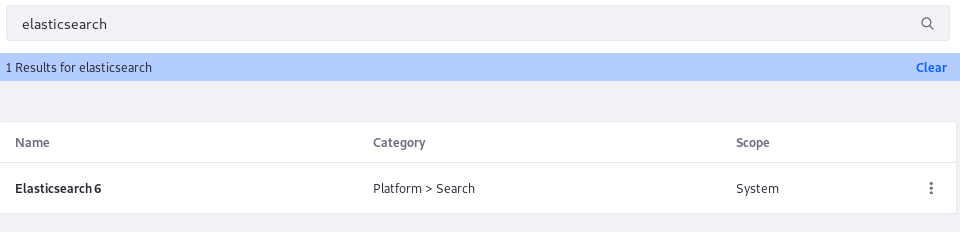
\includegraphics{./images/cfg-elasticsearch-sys-settings.png}
  \caption{Use the System Settings application in Liferay DXP's Control
  Panel to configure the Elasticsearch adapter.}
  \end{figure}
\item
  Make any edits to the configuration and click \emph{Save}.

  \begin{figure}
  \centering
  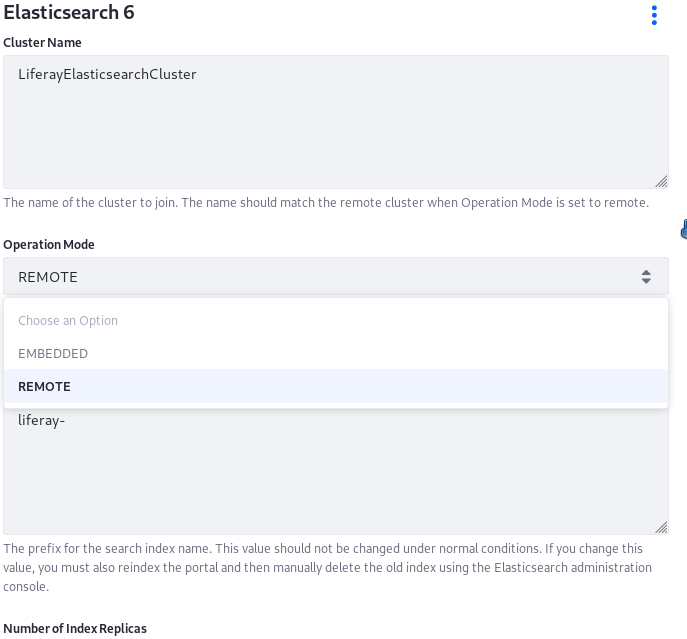
\includegraphics{./images/cfg-elasticsearch-sys-settings2.png}
  \caption{Set configurations for the Elasticsearch connector, like
  settings the Operation Mode to \emph{Remote}.}
  \end{figure}
\end{enumerate}

\noindent\hrulefill

\textbf{Note:} If you switch operation modes (\texttt{EMBEDDED} →
\texttt{REMOTE}), you must trigger a re-index. Navigate to \emph{Control
Panel} → \emph{Configuration} → \emph{Search}, and click \emph{Execute}
next to \emph{Reindex all search indexes.}

\noindent\hrulefill

\subsubsection{\texorpdfstring{Configuring the Adapter with an OSGi
\texttt{.config}
File}{Configuring the Adapter with an OSGi .config File}}\label{configuring-the-adapter-with-an-osgi-.config-file-1}

When preparing a system for production deployment, you should have a
repeatable deployment process. Therefore, it's best to use the OSGi
configuration file, where your configuration is maintained in a
controlled source.

Follow these steps to configure the Elasticsearch adapter using an OSGi
configuration file:

\begin{enumerate}
\def\labelenumi{\arabic{enumi}.}
\item
  Create the following file:

\begin{verbatim}
 [Liferay_Home]/osgi/configs/com.liferay.portal.search.elasticsearch6.configuration.ElasticsearchConfiguration.config
\end{verbatim}
\item
  Add configurations to the file, in the format
  \texttt{propertyName="Value"}. For example,

\begin{verbatim}
 operationMode="REMOTE"
 # If running Elasticsearch from a different computer:
 #transportAddresses="ip.of.elasticsearch.node:9300"
 # Highly recommended for all non-prodcution usage (e.g., practice, tests, diagnostics):
 #logExceptionsOnly="false"
\end{verbatim}
\item
  Start Liferay DXP or re-index if already running.
\end{enumerate}

As you can see from the System Settings entry for Elasticsearch, there
are a lot more configuration options available that help you tune your
system for optimal performance.

What follows here are some known good configurations for clustering
Elasticsearch. These, however, can't replace the manual process of
tuning, testing under load, and tuning again, so we encourage you to
examine the
\href{https://www.elastic.co/guide/en/elasticsearch/reference/6.1/important-settings.html}{Elasticsearch
documentation} and go through that process once you have a working
configuration.

\subsection{Configuring a Remote Elasticsearch
Host}\label{configuring-a-remote-elasticsearch-host-1}

In production systems Elasticsearch and Liferay DXP are installed on
different servers. To make Liferay DXP aware of the Elasticsearch
cluster, set

\begin{verbatim}
transportAddresses=[IP address of Elasticsearch Node]:9300
\end{verbatim}

Here's an example that sets the IP address of two nodes in the
Elasticsearch cluster:

\begin{verbatim}
transportAddresses=["192.168.1.1:9300","192.168.1.2:9300"]
\end{verbatim}

Set this in the Elasticsearch connector's OSGi configuration file. List
as many Elasticsearch nodes in this property as you want. This tells
Liferay DXP the IP address or host name where search requests should be
sent. If using System Settings, set the value in the \emph{Transport
Addresses} property.

\noindent\hrulefill

\textbf{Note:} In an Elasticsearch cluster you can list the transport
addresses for multiple Elasticsearch nodes as a comma-separated list in
the \texttt{transportAddresses} property. If you set only one transport
address, Liferay DXP loses contact with Elasticsearch if that node goes
down.

\noindent\hrulefill

On the Elasticsearch side, set the \texttt{network.host} property in
your \texttt{elaticsearch.yml} file. This property simultaneously sets
both the \emph{bind host} (the host where Elasticsearch listens for
requests) and the \emph{publish host} (the host name or IP address
Elasticsearch uses to communicate with other nodes). See
\href{https://www.elastic.co/guide/en/elasticsearch/reference/6.1/modules-network.html}{here}
for more information.

\subsection{Clustering Elasticsearch in Remote Operation
Mode}\label{clustering-elasticsearch-in-remote-operation-mode-1}

Clustering Elasticsearch is easy. First, set
\texttt{node.max\_local\_storage\_nodes} to be something greater than
\texttt{1}. When you run the Elasticsearch start script, a new local
storage node is added to the cluster. If you want four nodes running
locally, for example, run \texttt{./bin/elasticsearch} four times. See
\href{https://www.elastic.co/guide/en/elasticsearch/reference/6.1/modules-node.html\#max-local-storage-nodes}{here}
for more information.

Configure the number of shards and replicas in the Elasticsearch 6
adapter, using the \texttt{indexNumberOfShards} and
\texttt{indexNumberOfReplicas} properties to specify the number of
primary shards and number of replica shards, respectively.
Elasticsearch's default configuration works for a cluster of up to ten
nodes, since the default number of shards is \texttt{5} and the default
number of replica shards is \texttt{1}.

\noindent\hrulefill

\textbf{Note:} Elasticsearch uses the
\href{https://www.elastic.co/guide/en/elasticsearch/reference/6.1/modules-discovery-zen.html}{Zen
Discovery Module} by default, which provides unicast discovery.
Additionally, nodes in the cluster communicate using the
\href{https://www.elastic.co/guide/en/elasticsearch/reference/6.1/modules-transport.html}{Transport
Module}, through TCP. See the Elasticsearch documentation for the
available properties (to be set in the \texttt{elasticsearch.yml} file),
and the Liferay DXP Elasticsearch Adapter's settings for the adapter's
available settings.

At a minimum, provide the list of hosts (as \texttt{host:port}) to act
as gossip routers during unicast discovery in the
\texttt{elasticsearch.yml}:

\begin{verbatim}
 discovery.zen.ping.unicast.hosts: ["node1.ip.address", "node2.ip.address"]
\end{verbatim}

For example,

\begin{verbatim}
 discovery.zen.ping.unicast.hosts: ["10.10.10.5", "10.10.10,.5:9305"]
\end{verbatim}

\noindent\hrulefill

For more information on configuring an Elasticsearch cluster, see the
documentation on
\href{https://www.elastic.co/guide/en/elasticsearch/guide/current/_index_settings.html}{Elasticsearch
Index Settings}.

\subsection{Elasticsearch Connector System Settings, By Operation
Mode}\label{elasticsearch-connector-system-settings-by-operation-mode-1}

Some of the settings available for the Elasticsearch connector are
applicable for only one operation mode (REMOTe or EMBEDDED). Refer to
the table below:

Adapter Setting/Operation Mode \textbar{} EMBEDDED \textbar{} REMOTE
\textbar{} \texttt{clusterName} \textbar{} x \textbar{} x
\texttt{operationMode} \textbar{} x \textbar{} x
\texttt{indexNamePrefix} \textbar{} x \textbar{} x
\texttt{indexNumberOfReplicas*} \textbar{} x \textbar{} x
\texttt{indexNumberOfShards*} \textbar{} x \textbar{} x
\texttt{bootstrapMlockAll} \textbar{} x \textbar{} -
\texttt{logExceptionsOnly} \textbar{} x \textbar{} x
\texttt{retryOnConflict} \textbar{} x \textbar{} x
\texttt{discoveryZenPingUnicastHostsPort} \textbar{} x \textbar{} -
\texttt{networkHost} \textbar{} x \textbar{} - \texttt{networkBindHost}
\textbar{} x \textbar{} - \texttt{networkPublishHost} \textbar{} x
\textbar{} - \texttt{transportTcpPort} \textbar{} x \textbar{} -
\texttt{transportAddresses} \textbar{} - \textbar{} x
\texttt{clientTransportSniff} \textbar{} - \textbar{} x
\texttt{clientTransportIgnoreClusterName} \textbar{} - \textbar{} x
\texttt{clientTransportPingTimeout*} \textbar{} - \textbar{} x
\texttt{clientTransportNodesSamplerInterval} \textbar{} - \textbar{} x
\texttt{httpEnabled} \textbar{} x \textbar{} - \texttt{httpCORSEnabled}
\textbar{} x \textbar{} - \texttt{httpCORSAllowOrigin} \textbar{} x
\textbar{} - \texttt{httpCORSConfigurations} \textbar{} x \textbar{} -
\texttt{additionalConfigurations} \textbar{} x \textbar{} x
\texttt{additionalIndexConfigurations} \textbar{} x \textbar{} x
\texttt{additionalTypeMappings} \textbar{} x \textbar{} x
\texttt{overrideTypeMappings} \textbar{} x \textbar{} x
\texttt{syncSearch} \textbar{} x \textbar{} -

* \textbf{Note:} Available in the Connector to Elasticsearch 6 only.

1 This is, of course, a nod to all those fans of
\href{http://www.theatlantic.com/international/archive/2016/05/boaty-mcboatface-parliament-lessons/482046}{Boaty
Mcboatface}.

\section{Advanced Configuration of the Liferay Elasticsearch Connector
(6.1)}\label{advanced-configuration-of-the-liferay-elasticsearch-connector-6.1}

The default configurations for Liferay's Elasticsearch adapter module
are set in a Java class called \texttt{ElasticsearchConfiguration}.

While the Elasticsearch adapter has a lot of configuration options out
of the box, you might find an Elasticsearch configuration you need that
isn't provided by default. In this case, add the configuration options
you need. If something is configurable for Elasticsearch, its
configurable using the Elasticsearch adapter.

\subsection{Adding Settings and Mappings to the Liferay Elasticsearch
Adapter}\label{adding-settings-and-mappings-to-the-liferay-elasticsearch-adapter-1}

The available configuration options are divided into two groups: the
ones used most often by default and a catch-all for everything else. If
the necessary setting isn't available by default, you can still
configure it with the Liferay Elasticsearch adapter. Specify the
settings you need by using one or more of the
\texttt{additionalConfigurations},
\texttt{additionalIndexConfigurations}, or
\texttt{additionalTypeMappings}, and \texttt{overrideTypeMappings}
settings.

\begin{figure}
\centering
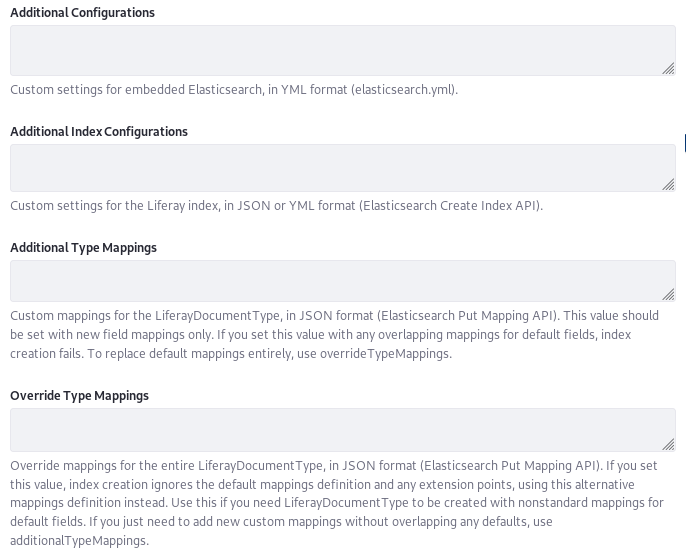
\includegraphics{./images/cfg-elasticsearch-additional-configs.png}
\caption{You can add Elasticsearch configurations to the ones currently
available in System Settings.}
\end{figure}

\texttt{additionalConfigurations} defines extra settings (in YAML) for
the embedded Elasticsearch. This is only useful for testing environments
using the embedded Elasticsearch server. Any node settings normally set
in \texttt{elasticsearch.yml} can be declared here. See the
\href{https://www.elastic.co/guide/en/elasticsearch/reference/6.1/index.html}{Elasticsearch
documentation} for a description of all possible node settings.

\texttt{additionalIndexConfigurations} defines extra settings (in JSON
or YAML) that are applied to the Liferay DXP index when it's created.
For example, you can create custom analyzers and filters using this
setting. For a complete list of available settings, see the
\href{https://www.elastic.co/guide/en/elasticsearch/reference/6.1/index-modules.html}{Elasticsearch
reference}.

Here's an example that shows how to configure
\href{https://www.elastic.co/guide/en/elasticsearch/guide/current/analysis-intro.html\#analysis-intro}{analysis}
that can be applied to a dynamic template (see below).

\begin{verbatim}
{  
    "analysis": {
        "analyzer": {
            "kuromoji_liferay_custom": {
                "filter": [
                    "cjk_width",
                    "kuromoji_baseform",
                    "pos_filter"
                ],
                "tokenizer": "kuromoji_tokenizer"
            }
        },
        "filter": {
            "pos_filter": {
                "type": "kuromoji_part_of_speech"
            }
        }
    }
}
\end{verbatim}

\texttt{additionalTypeMappings} defines extra field mappings for the
\texttt{LiferayDocumentType} type definition. These are applied when the
index is created. Add these field mappings in using JSON syntax. For
more information see
\href{https://www.elastic.co/guide/en/elasticsearch/reference/6.1/mapping.html}{here}
and
\href{https://www.elastic.co/guide/en/elasticsearch/reference/6.1/indices-put-mapping.html}{here}.
Use \texttt{additionalTypeMappings} for new field mappings, but do not
try to override existing \texttt{properties} mappings. If any of the
\texttt{properties} mappings set here overlap with existing mappings,
index creation fails. Use \texttt{overrideTypeMappings} to replace the
default \texttt{properties} mappings.

Here's an example of a
\href{https://www.elastic.co/guide/en/elasticsearch/reference/6.1/dynamic-templates.html}{dynamic
template} that uses the analysis configuration above to analyze all
string fields that end with \texttt{\_ja}.

\begin{verbatim}
{
    "LiferayDocumentType": {
        "dynamic_templates": [
            {
                "template_ja": {
                    "mapping": {
                        "analyzer": "kuromoji_liferay_custom",
                        "index": "analyzed",
                        "store": "true",
                        "term_vector": "with_positions_offsets",
                        "type": "string"
                    },
                    "match": "\\w+_ja\\b|\\w+_ja_[A-Z]{2}\\b",
                    "match_mapping_type": "string",
                    "match_pattern": "regex"
                }
            }
        ]
    }
}
\end{verbatim}

The above code adds a new \texttt{template\_ja} dynamic template. This
overrides the existing dynamic template with the same name. As with
dynamic templates, you can add sub-field mappings to Liferay DXP's type
mapping. These are referred to as
\href{https://www.elastic.co/guide/en/elasticsearch/reference/6.1/properties.html}{properties}
in Elasticsearch.

\begin{verbatim}
{ 
    "LiferayDocumentType": {  
        "properties": {   
            "fooName": {
                "index": "true",
                "store": "true",
                "type": "keyword"
            }
        }   
    }
}
\end{verbatim}

See
\href{https://www.elastic.co/guide/en/elasticsearch/reference/6.1/mapping-types.html}{here}
for more details on Elasticsearch's field datatypes.

The above example shows how a \texttt{fooName} field might be added to
Liferay DXP's type mapping. Because \texttt{fooName} is not an existing
property in the mapping, it works fine. If you try to override an
existing property mapping, index creation fails. Instead use the
\texttt{overrideTypeMappings} setting to override \texttt{properties} in
the mapping.

\textbf{Note:} To see that your additional mappings have been added to
the \texttt{LiferayDocumentType}, use \texttt{curl} to access this URL
after saving your additions and re-indexing:

\begin{verbatim}
curl http://[HOST]:[ES_PORT]/liferay-[COMPANY_ID]/_mapping/LiferayDocumentType?pretty
\end{verbatim}

Here's what it would look like for an Elasticsearch instance running on
\texttt{localhost:9200}, with a Liferay DXP Company ID of
\texttt{20116}:

\begin{verbatim}
curl http://localhost:9200/liferay-20116/_mapping/LiferayDocumentType?pretty
\end{verbatim}

In the above URL, \texttt{liferay-20116}is the index name. Including it
indicates that you want to see the mappings that were used to create the
index with that name.

\noindent\hrulefill

Use \texttt{overrideTypeMappings} to override Liferay DXP's default type
mappings. This is an advanced feature that should be used only if
strictly necessary. If you set this value, the default mappings used to
define the Liferay Document Type in Liferay DXP source code (for
example, \texttt{liferay-type-mappings.json}) are ignored entirely, so
include the whole mappings definition in this property, not just the
segment you're modifying. To make a modification, find the entire list
of the current mappings being used to create the index by navigating to
the URL

\begin{verbatim}
http://[HOST]:[ES_PORT]/liferay-[COMPANY_ID]/_mapping/LiferayDocumentType?pretty
\end{verbatim}

Copy the contents in as the value of this property (either into System
Settings or your OSGi configuration file). Leave the opening curly brace
\texttt{\{}, but delete lines 2-4 entirely:

\begin{verbatim}
"liferay-[COMPANY_ID]": {
    "mappings" : {
        "LiferayDocumentType" : {
\end{verbatim}

Then, from the end of the mappings, delete the concluding three curly
braces.

\begin{verbatim}
        }
    }
}
\end{verbatim}

Now modify whatever mappings you'd like. The changes take effect once
you save the changes and trigger a re-index from Server Administration.
If you need to add new custom mappings without overriding any defaults,
use \texttt{additionalTypeMappings} instead.

\subsection{Multi-line YAML
Configurations}\label{multi-line-yaml-configurations-1}

If you configure the settings from the last section using an OSGi
configuration file, you might find yourself needing to write YAML
snippets that span multiple lines. The syntax for that is
straightforward and just requires appending each line with
\texttt{\textbackslash{}n\textbackslash{}}, like this:

\begin{verbatim}
additionalConfigurations=\
                    cluster.routing.allocation.disk.threshold_enabled: false\n\
                    cluster.service.slow_task_logging_threshold: 600s\n\
                    index.indexing.slowlog.threshold.index.warn: 600s\n\
                    index.search.slowlog.threshold.fetch.warn: 600s\n\
                    index.search.slowlog.threshold.query.warn: 600s\n\
                    monitor.jvm.gc.old.warn: 600s\n\
                    monitor.jvm.gc.young.warn: 600s
\end{verbatim}

From simple configurations to overriding existing type mappings,
Elasticsearch and Liferay's connector to Elasticsearch are configurable.

\chapter{Installing Elasticsearch 7}\label{installing-elasticsearch-7}

Elasticsearrch 7 can be installed with Liferay DXP 7.1 (DXP-only). This
article presents a basic setup. For additional details on the general
Elasticsearch Installation procedure, refer to
\href{/docs/7-1/deploy/-/knowledge_base/d/installing-elasticsearch}{Installing
Elasticsearch}.

Once installed refere to the
\href{/docs/7-1/deploy/-/knowledge_base/d/configuring-the-liferay-elasticsearch-connector}{configuration
guide}.

\noindent\hrulefill

\textbf{Note:} Elasticsearch 6.x and 7.x are supported for 7.0. Refer to
the
\href{https://help.liferay.com/hc/en-us/articles/360016511651\#Liferay-DXP-7.1}{Search
Engine Compatibility Matrix} for details.

\noindent\hrulefill

To install Elasticsearch 7 on a new 7.0 installation:

\begin{enumerate}
\def\labelenumi{\arabic{enumi}.}
\item
  Install and configure Elasticsearch 7.x.
\item
  Install the Liferay Connector to Elasticsearch 7.
\item
  Disable the default, bundled Liferay Connector to Elasticsearch 6.
\item
  Configure Liferay DXP to connect to your Elasticsearch 7.x cluster.
\item
  Restart Liferay DXP and reindex your search indexes.
\end{enumerate}

\section{Install Elasticsearch}\label{install-elasticsearch}

To install Elasticsearch,

\begin{enumerate}
\def\labelenumi{\arabic{enumi}.}
\item
  Download an Elasticsearch archive (not the OSS version) from
  \href{https://www.elastic.co}{Elastic's website}.

  Download the latest Elasticsearch archive
  \href{https://help.liferay.com/hc/en-us/articles/360016511651\#Liferay-DXP-7.1}{compatible
  with your Liferay version}.
\item
  Extract the archive contents to a local folder where you want to run
  Elasticsearch. This folder is your \emph{Elasticsearch Home}.
\item
  Install the required Elasticsearch plugins by running these commands
  in your \texttt{{[}Elasticsearch\ Home{]}/bin} folder:

\begin{verbatim}
./elasticsearch-plugin install analysis-icu
\end{verbatim}

\begin{verbatim}
./elasticsearch-plugin install analysis-kuromoji
\end{verbatim}

\begin{verbatim}
./elasticsearch-plugin install analysis-smartcn
\end{verbatim}

\begin{verbatim}
./elasticsearch-plugin install analysis-stempel
\end{verbatim}
\end{enumerate}

Each Elasticsearch server is configured by its
\texttt{{[}Elasticsearch\ Home{]}/config/elasticsearch.yml} file.

Here's an example \texttt{elasticsearch.yml} configuration for a
single-node cluster:

\begin{verbatim}
cluster.name: LiferayElasticsearchCluster

discovery.type: single-node
network.host: es-network
node.name: es-node1
transport.port: 9300

# Include additional settings (e.g., security settings) 
\end{verbatim}

This cluster is named \texttt{LiferayElasticsearchCluster} and has one
node named \texttt{es-node1}.

If you are not configuring hosts for a production mode setup, use
\texttt{localhost} as the network host value. Elasticsearch can bind to
loopback addresses for HTTP and Transport communication. If you use a
loopback network address and single node discovery, this means the
Elasticsearch server is running in \emph{development mode}.

Start Elasticsearch.

\begin{verbatim}
./bin/elasticsearch
\end{verbatim}

\section{Install the Liferay Connector to Elasticsearch
7}\label{install-the-liferay-connector-to-elasticsearch-7}

Liferay requires installation of a connector application that can enable
communication with the corresponding Elasticsearch version:

\begin{enumerate}
\def\labelenumi{\arabic{enumi}.}
\item
  Download the
  \href{https://help.liferay.com/hc/en-us/articles/360016511651\#Liferay-DXP-7.1}{appropriate
  connector} for your version of Liferay and Elasticsearch.
\item
  Stop Liferay and place the LPKG file into
  \texttt{Liferay\ Home/osgi/marketplace/}.
\end{enumerate}

\section{Disable the default Liferay Connector to Elasticsearch
6}\label{disable-the-default-liferay-connector-to-elasticsearch-6}

Whether you're installing Elasticsearch 7 for a new 7.0 installation or
upgrading an existing stack to Elasticsearch 6, you must disable
Liferay's Elasticsearch 6 search modules bundled with the Liferay DXP by
default.

\begin{enumerate}
\def\labelenumi{\arabic{enumi}.}
\item
  Create a configuration file named

  com.liferay.portal.bundle.blacklist.internal.BundleBlacklistConfiguration.config
\item
  Give it these contents:

\begin{verbatim}
blacklistBundleSymbolicNames=[ \
    "com.liferay.portal.search.elasticsearch6.api", \
    "com.liferay.portal.search.elasticsearch6.impl", \
    "com.liferay.portal.search.elasticsearch6.spi", \
    "com.liferay.portal.search.elasticsearch6.xpack.security.impl", \
    "Liferay Connector to X-Pack Security [Elastic Stack 6.x] - Impl", \
    "Liferay Enterprise Search Security  - Impl" \
]
\end{verbatim}
\item
  Place the file in \texttt{Liferay\ Home/osgi/configs}.
\end{enumerate}

\noindent\hrulefill

\textbf{Note:} After disabling the Elasticsearch 6 connection, you'll
see exceptions in the Liferay log, because there's now no search engine
connection. This is fixed by the next step.

\noindent\hrulefill

\section{Configure Liferay}\label{configure-liferay}

Create a configuration file named

\begin{verbatim}
com.liferay.portal.search.elasticsearch7.configuration.ElasticsearchConfiguration.config
\end{verbatim}

Give it these contents:

\begin{verbatim}
operationMode="REMOTE"
transportAddresses=["localhost:9300"]
\end{verbatim}

This simple configuration leverages many default settings, but the
configuration is customizable. See the
\href{https://www.elastic.co/guide/en/elasticsearch/reference/7.12/modules-network.html\#transport-settings}{Elasticsearch
documentation} to learn about the available transport settings.

Learn more about the Liferay connector's corresponding configurations in
the
\href{/docs/7-1/deploy/-/knowledge_base/d/configuring-the-liferay-elasticsearch-connector}{configuration
guide}.

\section{Restart and Re-Index}\label{restart-and-re-index}

If both Liferay and Elasticsearch are running, once the connection is
configured the Elasticsearch log shows that the Liferay indexes are
created:

\begin{verbatim}
[2021-05-05T13:16:29,016][INFO ][o.e.c.m.MetadataCreateIndexService] [es-node1] [liferay-0] creating index, cause [api], templates [], shards [1]/[1]
[2021-05-05T13:16:29,032][INFO ][o.e.c.r.a.AllocationService] [es-node1] updating number_of_replicas to [0] for indices [liferay-0]
[2021-05-05T13:16:29,300][INFO ][o.e.c.r.a.AllocationService] [es-node1] Cluster health status changed from [YELLOW] to [GREEN] (reason: [shards started [[liferay-0][0]]]).
[2021-05-05T13:16:29,392][INFO ][o.e.c.m.MetadataMappingService] [es-node1] [liferay-0/rkLFWo4gT9mkL9Y2wrKkpA] update_mapping [LiferayDocumentType]
[2021-05-05T13:16:29,468][INFO ][o.e.c.m.MetadataMappingService] [es-node1] [liferay-0/rkLFWo4gT9mkL9Y2wrKkpA] update_mapping [LiferayDocumentType]
[2021-05-05T13:16:29,534][INFO ][o.e.c.m.MetadataCreateIndexService] [es-node1] [liferay-20099] creating index, cause [api], templates [], shards [1]/[1]
[2021-05-05T13:16:29,535][INFO ][o.e.c.r.a.AllocationService] [es-node1] updating number_of_replicas to [0] for indices [liferay-20099]
[2021-05-05T13:16:29,662][INFO ][o.e.c.r.a.AllocationService] [es-node1] Cluster health status changed from [YELLOW] to [GREEN] (reason: [shards started [[liferay-20099][0]]]).
[2021-05-05T13:16:29,722][INFO ][o.e.c.m.MetadataMappingService] [es-node1] [liferay-20099/214vtbkjTkmW_VCR_xOqyQ] update_mapping [LiferayDocumentType]
[2021-05-05T13:16:29,785][INFO ][o.e.c.m.MetadataMappingService] [es-node1] [liferay-20099/214vtbkjTkmW_VCR_xOqyQ] update_mapping [LiferayDocumentType]
\end{verbatim}

In the Control Panel, navigate to Configuration → Search and verify the
Elasticsearch connection is active.

\begin{figure}
\centering
\includegraphics{./images/elasticsearch-7-connection.png}
\caption{An active connection is displayed in the Search administrative
panel.}
\end{figure}

\noindent\hrulefill

\textbf{Important:} Re-index your search indexes and spell check
indexes. Invoke both of these actions in the Index Actions tab of
Control Panel → Configuration → Search.

\section{Upgrading to Elasticsearch
7}\label{upgrading-to-elasticsearch-7}

Elasticsearch 7 is supported for Liferay DXP 7.1. If you're upgrading
Liferay DXP and still running Elasticsearch 6, consider upgrading your
Elasticsearch servers too. If you're setting up a new system and not
already running a remote Elasticsearch 6 server, follow the
\href{/docs/7-1/deploy/-/knowledge_base/d/installing-elasticsearch-7}{installation
guide} to install Elasticsearch 7 and the
\href{/docs/7-1/deploy/-/knowledge_base/d/configuring-the-liferay-elasticsearch-connector}{configuration
guide} to configure the Elasticsearch adapter.

\noindent\hrulefill

\textbf{Before Proceeding,} back up your existing data before upgrading
Elasticsearch. If something goes wrong during or after the upgrade, roll
back to the previous version using the uncorrupted index snapshots. See
\href{/docs/7-1/deploy/-/knowledge_base/d/backing-up-elasticsearch}{here}
for more information.

\noindent\hrulefill

Here, you'll learn to upgrade an existing Elasticsearch 6 server (or
cluster) to Elasticsearch 7:

\begin{enumerate}
\def\labelenumi{\arabic{enumi}.}
\item
  \href{/docs/7-1/deploy/-/knowledge_base/d/installing-elasticsearch-7}{Install
  and configure Elasticsearch 7}.
\item
  In 7.0, security is now provided out of the box. If you're using
  X-Pack security, enable it (it's disabled by default):

\begin{verbatim}
xpack.security.enabled: true
\end{verbatim}
\item
  Blacklist the bundled Liferay Connector to Elasticsearch 6.
\item
  Install and configure the Liferay Connector to Elasticsearch 7.
\item
  Re-index all search and spell check indexes.
\end{enumerate}

Learn about configuring Elasticsearch
\href{/docs/7-1/deploy/-/knowledge_base/d/configuring-the-liferay-elasticsearch-connector}{here}.

\subsection{Blacklisting Elasticsearch
6}\label{blacklisting-elasticsearch-6}

To blacklist Elasticsearch 6,

\begin{enumerate}
\def\labelenumi{\arabic{enumi}.}
\item
  Create a configuration file named

\begin{verbatim}
com.liferay.portal.bundle.blacklist.internal.BundleBlacklistConfiguration.config
\end{verbatim}
\item
  Give it these contents:

\begin{verbatim}
blacklistBundleSymbolicNames=[ \
    "com.liferay.portal.search.elasticsearch6.api", \
    "com.liferay.portal.search.elasticsearch6.impl", \
    "com.liferay.portal.search.elasticsearch6.spi", \
    "com.liferay.portal.search.elasticsearch6.xpack.security.impl", \
    "Liferay Connector to X-Pack Security [Elastic Stack 6.x] - Impl", \
    "Liferay Enterprise Search Security  - Impl" \
]
\end{verbatim}
\end{enumerate}

\subsection{Re-index}\label{re-index}

Once the Elasticsearch adapter is installed and talking to the
Elasticsearch cluster, navigate to \emph{Control Panel} →
\emph{Configuration} → \emph{Search}, and click \emph{Execute} for the
\emph{Reindex all search indexes} entry.

You must also re-index the spell check indexes.

\subsection{Reverting to Elasticsearch
6}\label{reverting-to-elasticsearch-6}

Stuff happens. If that stuff involves an unrecoverable failure during
the upgrade to Elasticsearch 7, roll back to Elasticsearch 6 and
regroup.

Since your Elasticsearch 6 and 7 are currently two separate
installations, this procedure takes only a few steps:

\begin{enumerate}
\def\labelenumi{\arabic{enumi}.}
\item
  Stop the Liferay Connector to Elasticsearch 6.
\item
  Stop Elasticsearch 7 and make sure that the Elasticsearch 6
  \texttt{elasticsearch.yml} and the connector app are configured to use
  the same port (9200 by default).
\item
  Start the Elasticsearch server, and then restart the Liferay Connector
  to Elasticsearch 6.
\end{enumerate}

\chapter{Installing Liferay Enterprise
Search}\label{installing-liferay-enterprise-search}

A Liferay Enterprise Search (LES) subscription provides access to
additional search features beyond what's available out of the box with
your Liferay DXP subscription. To see a detailed description of the
services and features included with LES on Liferay DXP, refer to the
official description of LES in the
\href{https://help.liferay.com/hc/en-us/articles/360014400932}{Liferay
DXP Components resource}.

\noindent\hrulefill

\textbf{Note:} To install Cross-Cluster Replication with 7.0, follow the
instructions found on
\href{https://learn.liferay.com/dxp/latest/en/using-search/liferay-enterprise-search/cross-cluster-replication/cross-cluster-replication.html}{Liferay
Learn}. The procedure is nearly identical between Liferay 7.1 and 7.2,
with any differences noted inline in the Liferay Learn articles.

\noindent\hrulefill

LES customers receive a
\href{https://www.elastic.co/subscriptions}{platinum Elasticsearch
license} from Liferay. There can be a delay between your subscription
and receipt of the license, but you can enable a
\href{https://www.elastic.co/guide/en/elasticsearch/reference/7.x/start-trial.html}{30-day
trial} to work with in the meantime.

Detailed installation and usage instructions are available in the
article for each LES feature, including

\begin{itemize}
\tightlist
\item
  {[}Liferay Learn{]}
  \href{https://learn.liferay.com/dxp/latest/en/using-search/liferay-enterprise-search/cross-cluster-replication/cross-cluster-replication.html}{Cross-Cluster
  Replication}
\item
  \href{/docs/7-1/deploy/-/knowledge_base/d/monitoring-product}{Monitoring
  Elasticsearch}
\item
  \href{/docs/7-1/deploy/-/knowledge_base/d/installing-liferay-enterprise-search-security}{Securing
  Elasticsearch} {[}Free without LES for Liferay DXP with Elasticsearch
  7{]}
\end{itemize}

Always check the
\href{https://help.liferay.com/hc/en-us/articles/360016511651\#Liferay-Enterprise-Search}{LES
compatibility matrix} for compatibility information.

Here's an overview of using LES with Liferay DXP:

\begin{enumerate}
\def\labelenumi{\arabic{enumi}.}
\item
  Get an
  \href{https://help.liferay.com/hc/en-us/articles/360014400932}{Enterprise
  Search subscription}.
\item
  You'll receive a license for the Elasticsearch features. Install it on
  your Elasticsearch servers.
\item
  Download and install the
  \href{https://customer.liferay.com/downloads?p_p_id=com_liferay_osb_customer_downloads_display_web_DownloadsDisplayPortlet&_com_liferay_osb_customer_downloads_display_web_DownloadsDisplayPortlet_productAssetCategoryId=118191013&_com_liferay_osb_customer_downloads_display_web_DownloadsDisplayPortlet_fileTypeAssetCategoryId=118191060}{Liferay
  Enterprise Search apps} you purchased.
\item
  Configure the connectors with the proper credentials and encryption
  information.
\item
  Restart Elasticsearch.
\end{enumerate}

\chapter{Installing Liferay Enterprise Search
Security}\label{installing-liferay-enterprise-search-security}

\section{Enabling X-Pack Security}\label{enabling-x-pack-security}

\noindent\hrulefill

\textbf{Elasticsearch 6.x:} If you're using Elasticsearch 6, a Liferay
Enterprise Search (LES) subscription is required to use X-Pack Security
in your Liferay DXP-Elasticsearch stack. Starting with the \emph{Liferay
Connector to Elasticsearch 7} (available for Liferay DXP 7.1 on Liferay
Marketplace), X-Pack security is included by default. Liferay Enterprise
Search Monitoring still requires LES.

\noindent\hrulefill

The first thing to do is enable X-Pack security. Add this setting in
\texttt{elasticsearch.yml}:

\begin{verbatim}
xpack.security.enabled: true
\end{verbatim}

Now you can set up X-Pack users.

\section{Setting Up X-Pack Users in
Elasticsearch}\label{setting-up-x-pack-users-in-elasticsearch}

In a system using Security and Monitoring, Kibana and Liferay must
authenticate as clients to Elasticsearch, using the credentials
configured for these built-in X-Pack users:

\begin{itemize}
\tightlist
\item
  \texttt{kibana\_system}
\item
  \texttt{elastic}
\end{itemize}

Set the passwords for all X-Pack's
\href{https://www.elastic.co/guide/en/x-pack/6.5/setting-up-authentication.html\#built-in-users}{built-in
users}. The \texttt{setup-passwords} command is the simplest method to
set the built-in users' first-use passwords for the first time. To
update a password subsequently, use Kibana's UI or the
\href{https://www.elastic.co/guide/en/elasticsearch/reference/6.5/security-api-change-password.html}{Change
Password API}.

The \texttt{interactive} argument sets the passwords for all built-in
users. The configuration shown in these articles assumes you set all
passwords to \emph{liferay}. Of course, that's not recommended for
production systems.

\begin{verbatim}
./bin/elasticsearch-setup-passwords interactive
\end{verbatim}

Elastic's
\href{https://www.elastic.co/guide/en/elasticsearch/reference/6.5/setup-passwords.html}{setup-passwords
command} documentation describes additional options.

Since you're securing Elasticsearch, remember the \texttt{elastic}
user's password.

Enable transport layer security on each node.

\section{Encrypting Communications in
Elasticsearch}\label{encrypting-communications-in-elasticsearch}

The following instructions for enabling SSL/TLS use \texttt{liferay} as
the password whenever one is needed. Use your own passwords for your
installation.

\noindent\hrulefill

\textbf{Important:} Elasticsearch and Liferay DXP must share the keys
and certificates used to configure SSL. Copy them between servers and
point to the local copy in the corresponding configuration files.

\noindent\hrulefill

\subsection{Generate Node
Certificates}\label{generate-node-certificates}

\href{https://www.elastic.co/guide/en/elasticsearch/reference/7.x/configuring-tls.html\#node-certificates}{Generate
a certificate} for each node, or generate a certificate to be used on
all nodes and clients---like Liferay. Alternatively, use your
certificate authority to obtain node certificates.

\begin{enumerate}
\def\labelenumi{\arabic{enumi}.}
\item
  Generate X-Pack certificate authority using the X-Pack's
  \href{https://www.elastic.co/guide/en/elasticsearch/reference/7.x/certutil.html}{\texttt{certutil}}
  command:

\begin{verbatim}
./bin/elasticsearch-certutil ca --ca-dn CN=elastic-ca
\end{verbatim}

  This generates a file called \texttt{elastic-stack-ca.p12}.

  To generate the certificate authority cert and private key in PEM
  format,

\begin{verbatim}
./bin/elasticsearch-certutil ca --pem --ca-dn CN=elastic-ca
\end{verbatim}
\item
  Move the certificate authority file(s) file to the
  \texttt{{[}Elasticsearch\ \ \ \ Home{]}/config/certs} folder.
\item
  Generate X.509 certificates and private keys using the CA you created:

  To generate certificates and keys in \texttt{PKCS\#12} format, run

\begin{verbatim}
./bin/elasticsearch-certutil cert --ca config/certs/elastic-stack-ca.p12 --ca-pass liferay --dns localhost --ip 127.0.0.1 --name elastic-nodes
\end{verbatim}

  To generate certificates and keys in \texttt{PEM} format, run

\begin{verbatim}
./bin/elasticsearch-certutil cert --pem --ca-cert config/certs/ca.crt --ca-key config/certs/ca.key --dns localhost --ip 127.0.0.1 --name elastic-nodes
\end{verbatim}

  To generate \texttt{PEM} format node certificates and keys from the
  \texttt{PKSC\#12} certificate authority, run

\begin{verbatim}
./bin/elasticsearch-certutil cert --pem --ca config/certs/elastic-stack-ca.p12 --ca-pass liferay --dns localhost --ip 127.0.0.1 --name elastic-nodes
\end{verbatim}

  To generate a certificate that works with multiple hosts (for example
  to use the same certificate on all Elasticsearch and Liferay servers),
  use comma-separated lists when listing the DNS names and IP addresses:

\begin{verbatim}
./bin/elasticsearch-certutil cert --ca config/certs/elastic-stack-ca.p12 --ca-pass liferay --dns localhost,example.com,es-node1,es-node2,es-node3 --ip 127.0.0.1,<IPv4-address-2>,<IPv4-address-3>,<IPv4-address-4>
\end{verbatim}

  The \texttt{elasticsearch-certutil\ cert} command generates another
  file called \texttt{elastic-nodes.p12} (feel free to name it
  differently).
\end{enumerate}

\noindent\hrulefill

\begin{verbatim}
**Note:** The `certutil` command defaults to using the PKCS#12 format
for certificate generation, which works with your Elastic Stack 7.x. Kibana
6.x does not work with PKCS#12 certificates, so the `--pem` option
(generates the certificate in PEM format) is important if you're using
Liferay 7.1 and Kibana 6.x with *Liferay Enterprise Search Monitoring*. The
PEM command  for each case generates two ZIP files: `ca.crt` and
`ca.key`, `elastic-nodes.crt` and `elastic-nodes.key`. Unzip the
archive contents in `[Elasticsearch Home]/config/certs`.
\end{verbatim}

\noindent\hrulefill

\begin{enumerate}
\def\labelenumi{\arabic{enumi}.}
\item
  Move \texttt{elastic-nodes.p12} to the
  \texttt{{[}Elasticsearch\ Home{]}/config/certs} folder.

  \textbf{Checkpoint:} You now have the following files in your
  \texttt{{[}Elasticsearch\ \ Home{]}/config/certs} folder:

\begin{verbatim}
elastic-nodes.p12
elastic-stack-ca.p12
\end{verbatim}

  or

\begin{verbatim}
ca.crt
ca.key
elastic-nodes.crt
elastic-nodes.key
\end{verbatim}
\item
  Copy the files to the same folder on each Elasticsearch node, and to
  an appropriate location on each Liferay server node.
\end{enumerate}

The certificates and keys are ready to use in your Elasticsearch
configuration.

\subsection{Enable TLS in
Elasticsearch}\label{enable-tls-in-elasticsearch}

Enable TLS
(\href{https://www.elastic.co/guide/en/elasticsearch/reference/6.x/configuring-tls.html\#enable-ssl}{6.x},
\href{https://www.elastic.co/guide/en/elasticsearch/reference/7.x/configuring-tls.html}{7.x})
on each node via its
\texttt{{[}Elasticsearch\ Home{]}/config/elasticsearch.yml} file.

\begin{enumerate}
\def\labelenumi{\arabic{enumi}.}
\item
  Enable transport layer TLS with these settings in
  \texttt{elasticsearch.yml} for inter-node communication:

\begin{verbatim}
xpack.security.transport.ssl.enabled: true
\end{verbatim}
\item
  Add the certificate, key and certificate authority paths to each
  node's \texttt{elasticsearch.yml}:

\begin{verbatim}
# PKCS#12
xpack.security.transport.ssl.keystore.path: certs/elastic-nodes.p12
xpack.security.transport.ssl.keystore.password: liferay
xpack.security.transport.ssl.truststore.path: certs/elastic-nodes.p12
xpack.security.transport.ssl.truststore.password: liferay
xpack.security.transport.ssl.verification_mode: certificate
\end{verbatim}

  The example paths above assume you added the certificates to
  \texttt{{[}Elasticsearch\ Home{]}/config/certs}.
\item
  Enable TLS on the HTTP layer to encrypt client communication:

\begin{verbatim}
xpack.security.http.ssl.enabled: true
\end{verbatim}
\item
  Configure the certificate, key, and certificate authority paths to
  each node's \texttt{elasticsearch.yml}:

\begin{verbatim}
# PKCS#12
xpack.security.http.ssl.keystore.path: certs/elastic-nodes.p12
xpack.security.http.ssl.keystore.password: liferay
xpack.security.http.ssl.truststore.path: certs/elastic-nodes.p12
xpack.security.http.ssl.truststore.password: liferay
\end{verbatim}
\end{enumerate}

\noindent\hrulefill

\textbf{PEM:} To configure Elasticsearch using \texttt{PEM} format
certificates, refer to the examples below.

\noindent\hrulefill

Once TLS is enabled, configure X-Pack Security in Liferay DXP.

\section{Configuring Security in Liferay's Elasticsearch
Connector}\label{configuring-security-in-liferays-elasticsearch-connector}

\noindent\hrulefill

\textbf{Elasticsearch 6.x:} If you have a Liferay Enterprise Search
subscription,
\href{https://web.liferay.com/group/customer/dxp/downloads/enterprise-search}{download}
the Liferay Enterprise Search Security app. Install the LPKG file by
copying it into the \texttt{Liferay\ Home/deploy} folder.

\noindent\hrulefill

\noindent\hrulefill

\textbf{Elasticsearch 7.x:} The Liferay Connector to Elasticsearch 7
(DXP-only on Liferay 7.1) includes security integration by default;
installing the LES Security app is unnecessary.

\noindent\hrulefill

To configure security, navigate to \emph{Control Panel} →
\emph{Configuration} → \emph{System Settings}. Find the \emph{Search}
category and click on the \emph{X-Pack Security} entry. You can enter
the property values here, but it's more common to use a
\href{/docs/7-1/user/-/knowledge_base/u/understanding-system-configuration-files}{configuration
file} deployed to \texttt{{[}Liferay\ Home{]}/osgi/configs}.

On Elasticsearch 7.x, for the security adapter, create a file called

\begin{verbatim}
com.liferay.portal.search.elasticsearch7.configuration.XPackSecurityConfiguration.config
\end{verbatim}

For Elasticsearch 6.x installations the file is named

\begin{verbatim}
com.liferay.portal.search.elasticsearch6.xpack.security.internal.configuration.XPackSecurityConfiguration.config
\end{verbatim}

The exact contents of the file depend on your X-Pack setup in
Elasticsearch. To configure the adapter according to the Elasticsearch
setup documented here, populate the file like this (\texttt{PKCS\#12}):

\begin{verbatim}
certificateFormat="PKCS#12"
sslKeystorePath="/PATH/TO/elastic-nodes.p12"
sslKeystorePassword="liferay"
sslTruststorePath="/PATH/TO/elastic-nodes.p12"
sslTruststorePassword="liferay"
requiresAuthentication=B"true"
username="elastic"
password="liferay"
transportSSLVerificationMode="certificate"
transportSSLEnabled=B"true"
\end{verbatim}

Use settings like this if you're using \texttt{PEM} format certificates:

\begin{verbatim}
certificateFormat="PEM"
sslKeyPath="/PATH/TO/elastic-nodes.key"
sslCertificatePath="/PATH/TO/elastic-nodes.crt"
requiresAuthentication=B"true"
username="elastic"
password="liferay"
sslCertificateAuthoritiesPaths="/PATH/TO/ca.crt"
transportSSLVerificationMode="certificate"
transportSSLEnabled="true"
\end{verbatim}

Note that the \texttt{password} should match what you set during the
X-Pack password setup.

The certificate and key files referenced here are the same ones used on
the Elasticsearch server. Copy them to the Liferay DXP server and update
their paths in the configuration accordingly.

Enable authentication by setting \texttt{requiresAuthentication} to
\texttt{true} and providing the credentials for the Elasticsearch user.
For SSL, enable transport SSL, set the certificate verification mode and
certificate format, and provide the path to the certificate, key, and
certificate authority. Of course, the exact values depend on your X-Pack
configuration.

Here's the complete list of security configuration options:

\begin{itemize}
\tightlist
\item
  \texttt{sslKeyPath}
\item
  \texttt{sslCertificatePath}
\item
  \texttt{sslCertificateAuthoritiesPaths}
\item
  \texttt{certificateFormat}
\item
  \texttt{requiresAuthentication}
\item
  \texttt{username}
\item
  \texttt{password}
\item
  \texttt{transportSSLVerificationMode}
\item
  \texttt{transportSSLEnabled}
\item
  \texttt{sslKeystorePath}
\item
  \texttt{sslKeystorePassword}
\item
  \texttt{sslTruststorePath}
\item
  \texttt{sslTruststorePassword}
\end{itemize}

When you're finished configuring X-Pack Security, restart Elasticsearch.
These steps require a full cluster restart.

\section{Example Elasticsearch Security
Configurations}\label{example-elasticsearch-security-configurations}

Here are the complete Elasticsearch 7.x configurations from this article
(\texttt{elasticsearch.yml}; applies equally to Elasticsearch 6.5.x+):

\subsection{Example Elasticsearch Security Configuration -
PKCS\#12}\label{example-elasticsearch-security-configuration---pkcs12}

\begin{verbatim}
cluster.name: LiferayElasticsearchCluster

# X-Pack Security
xpack.security.enabled: true

## TLS/SSL settings for Transport layer (PKCS#12)
xpack.security.transport.ssl.enabled: true
xpack.security.transport.ssl.keystore.path: certs/elastic-nodes.p12
xpack.security.transport.ssl.keystore.password: liferay
xpack.security.transport.ssl.truststore.path: certs/elastic-nodes.p12
xpack.security.transport.ssl.truststore.password: liferay
xpack.security.transport.ssl.verification_mode: certificate

# TLS/SSL settings for HTTP layer (PKCS#12)
xpack.security.http.ssl.enabled: true
xpack.security.http.ssl.keystore.path: certs/elastic-nodes.p12
xpack.security.http.ssl.keystore.password: liferay
xpack.security.http.ssl.truststore.path: certs/elastic-nodes.p12
xpack.security.http.ssl.truststore.password: liferay

# Comment out when Kibana and Liferay's LES Monitoring are also configured
#xpack.monitoring.collection.enabled: true
\end{verbatim}

\section{Example Elasticsearch Security Configuration -
PEM}\label{example-elasticsearch-security-configuration---pem}

\begin{verbatim}
cluster.name: LiferayElasticsearchCluster

# X-Pack Security
xpack.security.enabled: true

## TLS/SSL settings for Transport layer (PEM)
xpack.security.transport.ssl.enabled: true
xpack.security.transport.ssl.certificate: certs/elastic-nodes.crt
xpack.security.transport.ssl.certificate_authorities: ["certs/ca.crt"]
xpack.security.transport.ssl.key: certs/elastic-nodes.key
xpack.security.transport.ssl.key_passphrase: liferay
xpack.security.transport.ssl.verification_mode: certificate

# TLS/SSL settings for HTTP layer (PEM)
xpack.security.http.ssl.enabled: true
xpack.security.http.ssl.certificate: certs/elastic-nodes.crt
xpack.security.http.ssl.certificate_authorities: ["certs/ca.crt"]
xpack.security.http.ssl.key: certs/elastic-nodes.key
xpack.security.http.ssl.key_passphrase: liferay

# Use this setting when Kibana and Liferay's LES Monitoring are also configured
#xpack.monitoring.collection.enabled: true
\end{verbatim}

\chapter{Installing Liferay Enterprise Search
Monitoring}\label{installing-liferay-enterprise-search-monitoring}

Monitor Elasticsearch with X-Pack Monitoring. First
\href{discover/deployment/-/knowledge_base-7-1/installing-x-pack}{install
X-Pack onto Elasticsearch} and configure security if you're using
X-Pack's security features. Then come back here for instructions on
installing and configuring Kibana (the monitoring server) with X-Pack so
that Elasticsearch (secured with X-Pack), Kibana (secured with X-Pack),
and Liferay DXP can communicate effortlessly and securely. A Liferay
Enterprise Search subscription is necessary for this integration.
Contact
\href{https://www.liferay.com/contact-us\#contact-sales}{Liferay's Sales
department for more information}.

\begin{enumerate}
\def\labelenumi{\arabic{enumi}.}
\item
  Tell Elasticsearch to enable data collection.
\item
  Download and install Kibana.
\item
  Configure Kibana with the proper security settings.
\item
  Install the
  \href{https://web.liferay.com/marketplace/-/mp/application/106163750}{Liferay
  Enterprise Search Monitoring}.
\item
  Configure the connector to communicate with Elasticsearch.
\end{enumerate}

This document assumes you're enabling security \emph{and} monitoring,
though differences in the process are noted as appropriate.

Start by enabling data collection in Elasticsearch.

\section{Enable Data Collection}\label{enable-data-collection}

Monitoring is enabled on Elasticsearch by default, but data collection
isn't. Enable data collection by adding this line to
\texttt{elasticsearch.yml}.

\begin{verbatim}
xpack.monitoring.collection.enabled: true
\end{verbatim}

Now install Kibana.

\section{Install Kibana}\label{install-kibana}

Make sure to install the correct version of Kibana. Check the
\href{https://web.liferay.com/group/customer/dxp/support/compatibility-matrix/enterprise-search}{Liferay
Enterprise Search compatibility matrix} for details.

\begin{enumerate}
\def\labelenumi{\arabic{enumi}.}
\item
  \href{https://www.elastic.co/downloads/kibana}{Download Kibana} and
  extract it. The root folder is referred to as \emph{Kibana Home}.
\item
  Tell Kibana where to send monitoring data by setting Elasticsearch's
  URL in \texttt{kibana.yml}:

\begin{verbatim}
elasticsearch.url: "http://localhost:9200"
\end{verbatim}

  If SSL is enabled on Elasticsearch, this is an \texttt{https} URL.
\item
  If not using X-Pack security, start Kibana by opening a command prompt
  to Kibana Home and entering this command:

\begin{verbatim}
./bin/kibana
\end{verbatim}
\end{enumerate}

If you're using X-Pack's security features on the Elasticsearch server,
there's additional configuration required before starting Kibana.

\subsection{Configure Kibana with
Authentication}\label{configure-kibana-with-authentication}

If X-Pack requires authentication to access the Elasticsearch cluster,
follow these steps or refer to
\href{https://www.elastic.co/guide/en/kibana/6.5/monitoring-xpack-kibana.html}{Elastic's
documentation}.

\begin{enumerate}
\def\labelenumi{\arabic{enumi}.}
\item
  Set the password for the built-in \texttt{kibana} user in
  \texttt{{[}Kibana\ \ \ \ \ Home{]}/config/kibana.yml}:

\begin{verbatim}
elasticsearch.username: "kibana"
elasticsearch.password: "liferay"
\end{verbatim}

  Use your \texttt{kibana} user password from your X-Pack setup. Once
  Kibana is installed, you can change the built-in user passwords from
  the \emph{Management} user interface.
\item
  If you're not encrypting communication with the Elasticsearch cluster,
  start Kibana from Kibana home.

\begin{verbatim}
./bin/kibana
\end{verbatim}
\item
  Go to \texttt{localhost:5601} and make sure you can sign in as a
  \href{https://www.elastic.co/guide/en/x-pack/6.5/native-realm.html\#native-add}{user}
  who has the \texttt{kibana\_user}
  \href{https://www.elastic.co/guide/en/x-pack/6.5/built-in-roles.html}{role}
  or a superuser (like the \texttt{elastic} user).
\end{enumerate}

\subsection{Configuring Kibana with
Encryption}\label{configuring-kibana-with-encryption}

Follow these steps to configure Kibana if X-Pack encrypts communication
with the Elasticsearch cluster. Consult
\href{https://www.elastic.co/guide/en/kibana/6.5/using-kibana-with-security.html\#using-kibana-with-security}{Elastic's
guide} for more information.

Add these settings to \texttt{kibana.yml}:

\begin{verbatim}
xpack.security.encryptionKey: "xsomethingxatxleastx32xcharactersx"
xpack.security.sessionTimeout: 600000

elasticsearch.ssl.verificationMode: certificate
elasticsearch.url: "https://localhost:9200"
elasticsearch.ssl.certificateAuthorities: [ "/path/to/ca.crt" ]

server.ssl.enabled: true
server.ssl.certificate: /path/to/[Elasticsearch Home]/config/localhost.crt
server.ssl.key: /path/to/[Elasticsearch Home]/config/localhost.key
\end{verbatim}

For more information about monitoring and security best practices in a
clustered environment, refer to
\href{https://www.elastic.co/guide/en/x-pack/6.5/secure-monitoring.html}{Elastic's
documentation}.

After this step you can access Kibana at \texttt{https://localhost:5601}
and sign in with a Kibana user. The last step is to connect Kibana to
Liferay DXP.

\section{Configuring the Liferay Enterprise Search Monitoring
App}\label{configuring-the-liferay-enterprise-search-monitoring-app}

If you have a Liferay Enterprise Search (Premium or Standard)
subscription, download the Liferay Enterprise Search Monitoring app.
Install the LPKG file by copying it into the
\texttt{Liferay\ Home/deploy} folder.

\begin{enumerate}
\def\labelenumi{\arabic{enumi}.}
\item
  Once the connector is installed and Kibana and Elasticsearch are
  securely configured, create a
  \href{/docs/7-1/user/-/knowledge_base/u/understanding-system-configuration-files}{configuration
  file} named

\begin{verbatim}
com.liferay.portal.search.elasticsearch6.xpack.monitoring.web.internal.configuration.XPackMonitoringConfiguration.config
\end{verbatim}
\item
  Place these settings in the \texttt{.config} file:

\begin{verbatim}
kibanaPassword="liferay"
kibanaUserName="elastic"
kibanaURL="http://localhost:5601"
\end{verbatim}

  The values depend on your Kibana configuration. For example, use a
  secure URL such as \texttt{kibanaURL="https://localhost:5601"} if
  you're using X-Pack Security features.

  Alternatively, configure the monitoring adapter from
  \href{/docs/7-1/user/-/knowledge_base/u/system-settings}{System
  Settings}. Navigate to \emph{Control Panel} → \emph{Configuration} →
  \emph{System Settings} and find the X-Pack Monitoring entry in the
  Search category. All the configuration options for the monitoring
  connector appear there.
\item
  Deploy this configuration file to \texttt{Liferay\ Home/osgi/configs},
  and your running instance applies the settings. There's no need to
  restart the server.
\item
  There are two more settings to add to Kibana itself. The first forbids
  Kibana from rewriting requests prefixed with \texttt{server.basePath}.
  The second sets Kibana's base path for the Monitoring portlet to act
  as a proxy for Kibana's monitoring UI. Add this to
  \texttt{kibana.yml}:

\begin{verbatim}
server.rewriteBasePath: false
server.basePath: "/o/portal-search-elasticsearch-xpack-monitoring/xpack-monitoring-proxy"
\end{verbatim}

  Note that once you set the \texttt{server.basePath}, you cannot access
  the Kibana UI through Kibana's URL (e.g.,
  \texttt{https://localhost:5601}). All access to the Kibana UI is
  through the Monitoring portlet, which is only accessible to signed in
  Liferay DXP users. Navigate directly to the portlet using this URL:

  \url{http://localhost:8080/o/portal-search-elasticsearch-xpack-monitoring/xpack-monitoring-proxy/app/monitoring}
\item
  Because you're using the Monitoring portlet in Liferay DXP as a proxy
  to Kibana's UI, if you are using X-Pack Security, you must configure
  the application server's startup JVM parameters to recognize a valid
  \emph{truststore} and \emph{password}.

  First, navigate to Elasticsearch Home and generate a PKSC\#12
  certificate from the CA you created when setting up X-Pack security:

\begin{verbatim}
./bin/elasticsearch-certutil cert --ca-cert /path/to/ca.crt --ca-key /path/to/ca.key --ip 127.0.0.1 --dns localhost --name localhost --out /path/to/Elasticsearch_Home/config/localhost.p12
\end{verbatim}

  Next use the \texttt{keytool} command to generate a truststore:

\begin{verbatim}
keytool -importkeystore -deststorepass liferay -destkeystore /path/to/truststore.jks -srckeystore /path/to/Elasticsearch_Home/config/localhost.p12 -srcstoretype PKCS12 -srcstorepass liferay
\end{verbatim}

  Add the trustore path and password to your application server's
  startup JVM parameters. Here are example truststore and path
  parameters for appending to a Tomcat server's \texttt{CATALINA\_OPTS}:

\begin{verbatim}
-Djavax.net.ssl.trustStore=/path/to/truststore.jks -Djavax.net.ssl.trustStorePassword=liferay
\end{verbatim}
\end{enumerate}

Restart Liferay DXP and Kibana.

\section{Monitoring in Liferay DXP}\label{monitoring-in-liferay-dxp}

Once Kibana and X-Pack are successfully installed and configured and all
the servers are running, add the X-Pack Monitoring portlet to a page:

\begin{enumerate}
\def\labelenumi{\arabic{enumi}.}
\item
  Open the \emph{Add} menu on a page and choose \emph{Widgets}
\item
  Search for \emph{monitoring} and drag the \emph{X-Pack Monitoring}
  widget from the Search category onto the page.
\end{enumerate}

See the Elastic documentation for information on
\href{https://www.elastic.co/guide/en/elasticsearch/reference/6.5/es-monitoring.html}{monitoring
Elasticsearch}.

\chapter{Installing X-Pack (6.1)}\label{installing-x-pack-6.1}

X-Pack is an
\href{https://www.elastic.co/guide/en/elasticsearch/reference/6.1/setup-xpack.html}{Elasticsearch
extension} for securing and monitoring Elasticsearch clusters. If you
use Elasticsearch, you should secure it with X-Pack. X-Pack's security
features include authenticating access to the Elasticsearch cluster's
data and encrypting Elasticsearch's internal and external
communications. Most production systems requires these features. A
Liferay Enterprise Search subscription gets you access to two X-Pack
Connectors for Liferay DXP: monitoring and security. Contact
\href{https://www.liferay.com/contact-us\#contact-sales}{Liferay's Sales
department for more information}.

Here's an overview of using X-Pack to secure the data indexed in
Elasticsearch:

\begin{enumerate}
\def\labelenumi{\arabic{enumi}.}
\item
  Get an Enterprise Search subscription.
\item
  \href{https://www.elastic.co/guide/en/x-pack/6.1/installing-xpack.html}{Install
  X-Pack into Elasticsearch} and configure it to require authentication
  and
  \href{https://www.elastic.co/guide/en/elasticsearch/reference/6.1/configuring-tls.html\#configuring-tls}{encryption}.
\item
  Download and install the
  \href{https://web.liferay.com/group/customer/dxp/downloads/enterprise-search}{Liferay
  Enterprise Search Security}.
\item
  Configure the secuirty app with the proper credentials and encryption
  information.
\item
  Restart Elasticsearch.
\end{enumerate}

\textbf{Important:} These steps require a full cluster restart.

On completing these steps, your Elasticsearch installation communicates
freely with Liferay DXP.

\noindent\hrulefill

\href{https://www.elastic.co/guide/en/elasticsearch/reference/6.1/configuring-security.html}{Elastic's
documentation} describes the X-Pack architecture and additional
configuration options and features.

\section{Installing X-Pack}\label{installing-x-pack}

Here are the X-Pack installation steps:

\begin{enumerate}
\def\labelenumi{\arabic{enumi}.}
\item
  To
  \href{https://www.elastic.co/guide/en/elasticsearch/reference/6.1/installing-xpack-es.html}{install
  X-Pack} and automatically grant it the required permissions
  (recommended), run this command on each Elasticsearch node:

\begin{verbatim}
bin/elasticsearch-plugin install x-pack --batch
\end{verbatim}

  The \texttt{-\/-batch} option bypasses installation prompts for
  granting permissions to X-Pack.

  The log output details the permissions granted and finishes with
  \texttt{Installed\ x-pack}:

\begin{verbatim}
-> Downloading x-pack from elastic
[=================================================] 100%   
@@@@@@@@@@@@@@@@@@@@@@@@@@@@@@@@@@@@@@@@@@@@@@@@@@@@@@@@@@@
@     WARNING: plugin requires additional permissions     @
@@@@@@@@@@@@@@@@@@@@@@@@@@@@@@@@@@@@@@@@@@@@@@@@@@@@@@@@@@@
* java.io.FilePermission \\.\pipe\* read,write
* java.lang.RuntimePermission accessClassInPackage.com.sun.activation.registries
* java.lang.RuntimePermission getClassLoader
* java.lang.RuntimePermission setContextClassLoader
* java.lang.RuntimePermission setFactory
* java.net.SocketPermission * connect,accept,resolve
* java.security.SecurityPermission createPolicy.JavaPolicy
* java.security.SecurityPermission getPolicy
* java.security.SecurityPermission putProviderProperty.BC
* java.security.SecurityPermission setPolicy
* java.util.PropertyPermission * read,write
See http://docs.oracle.com/javase/8/docs/technotes/guides/security/permissions.html
for descriptions of what these permissions allow and the associated risks.
@@@@@@@@@@@@@@@@@@@@@@@@@@@@@@@@@@@@@@@@@@@@@@@@@@@@@@@@@@@
@        WARNING: plugin forks a native controller        @
@@@@@@@@@@@@@@@@@@@@@@@@@@@@@@@@@@@@@@@@@@@@@@@@@@@@@@@@@@@
This plugin launches a native controller that is not subject to the Java
security manager nor to system call filters.
Elasticsearch keystore is required by plugin [x-pack], creating...
-> Installed x-pack
\end{verbatim}

  See more about the permissions X-Pack needs
  \href{https://www.elastic.co/guide/en/elasticsearch/reference/6.1/installing-xpack-es.html}{here}.
\item
  Make sure Elasticsearch does not allow automatic index creation by
  verifying this property in your \texttt{elasticsearch.yml} file:

\begin{verbatim}
action.auto_create_index: false
\end{verbatim}

  This property is \texttt{true} by default.
  \href{https://www.elastic.co/guide/en/elasticsearch/reference/6.1/docs-index_.html\#index-creation}{Elastic's
  documentation} describes more automatic index creation details.
\item
  Shutdown Liferay DXP and restart Elasticsearch.
\end{enumerate}

Now configure security and/or monitoring, depending on your needs.

\section{Installing X-Pack Security
(6.1)}\label{installing-x-pack-security-6.1}

Once X-Pack is installed, start securing Elasticsearch by configuring
the built-in user passwords.

\subsection{Setting Up X-Pack Users}\label{setting-up-x-pack-users}

In a system using X-Pack Security and X-Pack Monitoring, these built-in
X-Pack users are important:

\begin{itemize}
\tightlist
\item
  \texttt{kibana}
\item
  \texttt{elastic}
\end{itemize}

Set the passwords for all X-Pack's
\href{https://www.elastic.co/guide/en/x-pack/6.1/setting-up-authentication.html\#built-in-users}{built-in
users}. The \texttt{setup-passwords} command is the simplest method to
set the built-in users first-use passwords for the first time. To update
a password subsequently, use Kibana's UI or the
\href{https://www.elastic.co/guide/en/elasticsearch/reference/6.1/security-api-change-password.html}{Change
Password API}.

The \texttt{interactive} argument sets the passwords for all built-in
users. The configuration shown in these articles assumes you set all
passwords to \emph{liferay}. Of course, that's not recommended for
production systems.

\begin{verbatim}
./bin/x-pack/setup-passwords interactive
\end{verbatim}

Elastic's
\href{https://www.elastic.co/guide/en/elasticsearch/reference/6.1/setup-passwords.html}{setup-passwords
command} documentation describes additional options.

Since you're securing Elasticsearch, remember the \texttt{elastic}
user's password.

Enable transport layer security on each node.

\subsection{Enabling Transport Layer
Security}\label{enabling-transport-layer-security}

The following instructions for enabling TLS use \texttt{liferay} as the
password whenever one is needed. Use your own passwords for your
installation.

\subsubsection{Generate Node
Certificates}\label{generate-node-certificates-1}

\href{https://www.elastic.co/guide/en/elasticsearch/reference/6.1/configuring-tls.html\#node-certificates}{Generate
a node certificate} for each node. You can, of course, use a Certificate
Authority to obtain node certificates.

\begin{enumerate}
\def\labelenumi{\arabic{enumi}.}
\item
  Create a certificate authority, using
  \href{https://www.elastic.co/guide/en/elasticsearch/reference/6.1/certutil.html}{X-Pack's
  \texttt{certutil}} command:

\begin{verbatim}
./bin/x-pack/certutil ca --pem --ca-dn CN=localhost
\end{verbatim}

  This generates a ZIP file. Unzip the contents somewhere safe.
\item
  Generate X.509 certificates and private keys using the CA from Step 1.
  For example:

\begin{verbatim}
./bin/x-pack/certutil cert --pem --ca-cert /path/to/ca.crt --ca-key /path/to/ca.key --dns localhost --ip 127.0.0.1 --name localhost
\end{verbatim}

  This generates another ZIP file. Extract the contents somewhere in the
  \texttt{Elasticsearch\ Home/config} folder.
\end{enumerate}

\noindent\hrulefill

\textbf{Note:} The \texttt{certutil} command defaults to using the
\emph{PKSC\#12} format for certificate generation. Since Kibana does not
work with PKSC\#12 certificates, the \texttt{-\/-pem} option (generates
the certificate in PEM format) is important if you're using monitoring.

\noindent\hrulefill

\subsubsection{Enable TLS}\label{enable-tls}

\href{https://www.elastic.co/guide/en/elasticsearch/reference/6.1/configuring-tls.html\#enable-ssl}{Enable
TLS} on each node via its \texttt{elasticsearch.yml}.

\begin{enumerate}
\def\labelenumi{\arabic{enumi}.}
\item
  Add the certificate, key and certificate authority paths to each
  node's \texttt{elasticsearch.yml}:

\begin{verbatim}
xpack.ssl.certificate: /path/to/[Elasticsearch Home]/config/localhost.crt
xpack.ssl.key: /path/to/[Elasticsearch Home]/config/localhost.key
xpack.ssl.certificate_authorities: ["/path/to/ca.crt"]
\end{verbatim}

  The example paths above assume you added the certificate to
  \texttt{Elasticsearch\ Home/config/}.
\item
  Enable transport layer TLS with these settings in
  \texttt{elasticsearch.yml}:

\begin{verbatim}
xpack.security.transport.ssl.enabled: true
xpack.security.transport.ssl.verification_mode: certificate
\end{verbatim}
\item
  Enable TLS on the HTTP layer to encrypt client communication:

\begin{verbatim}
xpack.security.http.ssl.enabled: true
\end{verbatim}
\end{enumerate}

After X-Pack is installed and TLS is enabled, configure the security
adapter in Liferay DXP.

\subsection{Install and Configure the Liferay Enterprise Search Security
app}\label{install-and-configure-the-liferay-enterprise-search-security-app}

If you have a Liferay Enterprise Search subscription,
\href{https://web.liferay.com/group/customer/dxp/downloads/enterprise-search}{download}
the Liferay Enterprise Search Security app. Install the LPKG file by
copying it into the \texttt{Liferay\ Home/deploy} folder. That's all
there is to it.

To configure the security adapter, navigate to \emph{Control Panel} →
\emph{Configuration} → \emph{System Settings}. Find the \emph{Search}
category and click on the \emph{X-Pack Security} entry. You can enter
the property values here, but it's more common to use a
\href{/docs/7-1/user/-/knowledge_base/u/understanding-system-configuration-files}{configuration
file} deployed to \texttt{Liferay\ Home/osgi/configs}. For the security
adapter, create a file called

\begin{verbatim}
com.liferay.portal.search.elasticsearch6.xpack.security.internal.configuration.XPackSecurityConfiguration.config
\end{verbatim}

The exact contents of the file depend on your X-Pack setup. To configure
the adapter according to the Elasticsearch setup documented here,
populate the file like this:

\begin{verbatim}
sslKeyPath="/path/to/localhost.key"
sslCertificatePath="/path/to/localhost.crt"
certificateFormat="PEM"
requiresAuthentication="true"
username="elastic"
password="liferay"
sslCertificateAuthoritiesPaths="/path/to/ca.crt"
transportSSLVerificationMode="certificate"
transportSSLEnabled="true"
\end{verbatim}

Note that the \texttt{password} should match what you set during the
X-Pack password setup above.

The certificate and key files referenced here are the same ones used on
the Elasticsearch server. Copy them to the Liferay DXP server and update
their paths in the configuration accordingly.

Enable authentication by setting authentication to \texttt{required} and
providing the credentials for the Elasticsearch user. For SSL, enable
transport SSL, set the certificate verification mode and certificate
format, and provide the path to the certificate, key, and certificate
authority. Of course, the exact values depend on your X-Pack
configuration.

Here's the complete list of configuration options for the security app:

\begin{itemize}
\tightlist
\item
  \texttt{sslKeyPath}
\item
  \texttt{sslCertificatePath}
\item
  \texttt{sslCertificateAuthoritiesPaths}
\item
  \texttt{certificateFormat}
\item
  \texttt{requiresAuthentication}
\item
  \texttt{username}
\item
  \texttt{password}
\item
  \texttt{transportSSLVerificationMode}
\item
  \texttt{transportSSLEnabled}
\item
  \texttt{sslKeystorePath}
\item
  \texttt{sslKeystorePassword}
\item
  \texttt{sslTruststorePath}
\item
  \texttt{sslTruststorePassword}
\end{itemize}

When you're finished configuring security, restart Elasticsearch. These
steps require a full cluster restart.

\section{Installing X-Pack Monitoring
(6.1)}\label{installing-x-pack-monitoring-6.1}

Monitor Elasticsearch with X-Pack Monitoring. First
\href{discover/deployment/-/knowledge_base-7-1/installing-x-pack}{install
X-Pack onto Elasticsearch} and configure security if you're using
X-Pack's security features. Then come back here for instructions on
installing and configuring Kibana (the monitoring server) with X-Pack so
that Elasticsearch (secured with X-Pack), Kibana (secured with X-Pack),
and Liferay DXP can communicate effortlessly and securely. A Liferay
Enterprise Search subscription is necessary for this integration.
Contact
\href{https://www.liferay.com/contact-us\#contact-sales}{Liferay's Sales
department for more information}.

\begin{enumerate}
\def\labelenumi{\arabic{enumi}.}
\item
  Download and install Kibana.
\item
  Install X-Pack onto Kibana and configure Kibana with the proper
  security settings.
\item
  Download and install the
  \href{https://www.liferay.com/marketplace}{Liferay Enterprise Search
  Monitoring} app.
\item
  Configure the connector to communicate with Elasticsearch.
\end{enumerate}

This document assumes you're enabling security \emph{and} monitoring,
though differences in the process are noted as appropriate.

For the X-Pack installation procedure, refer to the
\href{/docs/7-1/deploy/-/knowledge_base/d/installing-x-pack-security-6-1}{security
article}.

Start with the installation of Kibana.

\subsection{Install Kibana}\label{install-kibana-1}

Make sure to install the correct version of Kibana. Check the
\href{https://help.liferay.com/hc/en-us/articles/360016511651\#Liferay-Enterprise-Search}{Liferay
Enterprise Search compatibility matrix} for details.

\begin{enumerate}
\def\labelenumi{\arabic{enumi}.}
\item
  \href{https://www.elastic.co/downloads/kibana}{Download Kibana} and
  extract it. The root folder is referred to as \emph{Kibana Home}.
\item
  Install X-Pack into Kibana:

\begin{verbatim}
./bin/kibana-plugin install x-pack
\end{verbatim}
\item
  Tell Kibana where to send monitoring data by setting Elasticsearch's
  URL in \texttt{kibana.yml}:

\begin{verbatim}
elasticsearch.url: "http://localhost:9200"
\end{verbatim}

  If SSL is enabled on Elasticsearch, this is an \texttt{https} URL.
\item
  If not using X-Pack security, start Kibana by opening a command prompt
  to Kibana Home and entering this command:

\begin{verbatim}
./bin/kibana
\end{verbatim}
\end{enumerate}

If you're using X-Pack's security features on the Elasticsearch server,
there's additional configuration required before starting Kibana.

\subsubsection{Configure Kibana with
Authentication}\label{configure-kibana-with-authentication-1}

If X-Pack requires authentication to access the Elasticsearch cluster,
follow these steps or refer to
\href{https://www.elastic.co/guide/en/kibana/6.1/monitoring-xpack-kibana.html}{Elastic's
documentation}.

\begin{enumerate}
\def\labelenumi{\arabic{enumi}.}
\item
  Set the password for the built-in \texttt{kibana} user in
  \texttt{Kibana\ \ \ \ \ Home/config/kibana.yml}:

\begin{verbatim}
elasticsearch.username: "kibana"
elasticsearch.password: "liferay"
\end{verbatim}

  Use your \texttt{kibana} user password from your X-Pack setup. Once
  Kibana is installed, you can change the built-in user passwords from
  the \emph{Management} user interface.
\item
  If you're not encrypting communication with the Elasticsearch cluster,
  start Kibana from Kibana home.

\begin{verbatim}
./bin/kibana
\end{verbatim}
\item
  Go to \texttt{localhost:5601} and make sure you can sign in as a\\
  \href{https://www.elastic.co/guide/en/x-pack/6.1/native-realm.html\#native-add}{user}
  who has the \texttt{kibana\_user}
  \href{https://www.elastic.co/guide/en/x-pack/6.1/built-in-roles.html}{role}.
\end{enumerate}

\subsubsection{Configuring Kibana with
Encryption}\label{configuring-kibana-with-encryption-1}

Follow these steps to configure Kibana if X-Pack encrypts communication
with the Elasticsearch cluster. Consult
\href{https://www.elastic.co/guide/en/kibana/6.1/using-kibana-with-security.html\#using-kibana-with-security}{Elastic's
guide} for more information.

Add these settings to \texttt{kibana.yml}:

\begin{verbatim}
xpack.security.encryptionKey: "xsomethingxatxleastx32xcharactersx"
xpack.security.sessionTimeout: 600000

elasticsearch.ssl.verificationMode: certificate
elasticsearch.url: "https://localhost:9200"
elasticsearch.ssl.certificateAuthorities: [ "/path/to/ca.crt" ]

server.ssl.enabled: true
server.ssl.certificate: /path/to/[Elasticsearch Home]/config/localhost.crt
server.ssl.key: /path/to/[Elasticsearch Home]/config/localhost.key
\end{verbatim}

For more information about monitoring and security best practices in a
clustered environment, refer to
\href{https://www.elastic.co/guide/en/x-pack/6.1/secure-monitoring.html}{Elastic's
documentation}.

After this step you can access Kibana at \texttt{https://localhost:5601}
and sign in with a Kibana user. The last step is to hook Kibana up with
Liferay DXP.

\subsection{Configuring the Liferay Enterprise Search Monitoring
App}\label{configuring-the-liferay-enterprise-search-monitoring-app-1}

If you have a Liferay Enterprise Search (Premium or Standard)
subscription, download the Liferay Enterprise Search Monitoring app.
Install the LPKG file by copying it into the
\texttt{Liferay\ Home/deploy} folder.

\begin{enumerate}
\def\labelenumi{\arabic{enumi}.}
\item
  Once the connector is installed and Kibana and Elasticsearch are
  securely configured, create a
  \href{/docs/7-1/user/-/knowledge_base/u/understanding-system-configuration-files}{configuration
  file} named

\begin{verbatim}
com.liferay.portal.search.elasticsearch6.xpack.monitoring.web.internal.configuration.XPackMonitoringConfiguration.config
\end{verbatim}
\item
  Place these settings in the \texttt{.config} file:

\begin{verbatim}
kibanaPassword="liferay"
kibanaUserName="elastic"
kibanaURL="http://localhost:5601"
\end{verbatim}

  The values depend on your Kibana configuration. For example, use a
  secure URL such as \texttt{kibanaURL="https://localhost:5601"} if
  you're using X-Pack Security features.

  Alternatively, configure the monitoring adapter from
  \href{/docs/7-1/user/-/knowledge_base/u/system-settings}{System
  Settings}. Navigate to \emph{Control Panel} → \emph{Configuration} →
  \emph{System Settings} and find the X-Pack Monitoring entry in the
  Search category. All the configuration options for the monitoring
  connector appear there.
\item
  Deploy this configuration file to \texttt{Liferay\ Home/osgi/configs},
  and your running instance applies the settings. There's no need to
  restart the server.
\item
  There's one more setting to add to Kibana itself. It sets Kibana's
  base path to let the Monitoring Portlet act as a proxy for Kibana's
  monitoring UI. Add this to \texttt{kibana.yml}:

\begin{verbatim}
server.basePath: "/o/portal-search-elasticsearch-xpack-monitoring/xpack-monitoring-proxy"
\end{verbatim}

  Note that once you set the \texttt{server.basePath}, you cannot access
  the Kibana UI through Kibana's URL (for example,
  \texttt{https://localhost:5601}). All access to the Kibana UI is
  through the Monitoring portlet, which is only accessible to logged in
  Liferay DXP users. Navigate directly to the portlet using this URL:

  \url{http://localhost:8080/o/portal-search-elasticsearch-xpack-monitoring/xpack-monitoring-proxy/app/monitoring}
\item
  Because you're using the Monitoring portlet in Liferay DXP as a proxy
  to Kibana's UI, if you are using X-Pack Security, you must configure
  the application server's startup JVM parameters to recognize a valid
  \emph{truststore} and \emph{password}.

  First, navigate to Elasticsearch Home and generate a PKSC\#12
  certificate from the CA you created when setting up X-Pack security:

\begin{verbatim}
./bin/x-pack/certutil cert --ca-cert /path/to/ca.crt --ca-key /path/to/ca.key --ip 127.0.0.1 --dns localhost --name localhost --out /path/to/Elasticsearch_Home/config/localhost.p12
\end{verbatim}

  Next use the \texttt{keytool} command to generate a truststore:

\begin{verbatim}
keytool -importkeystore -deststorepass liferay -destkeystore /path/to/truststore.jks -srckeystore /path/to/Elasticsearch_Home/config/localhost.p12 -srcstoretype PKCS12 -srcstorepass liferay
\end{verbatim}

  Add the trustore path and password to your application server's
  startup JVM parameters. Here are example truststore and path
  parameters for appending to a Tomcat server's \texttt{CATALINA\_OPTS}:

\begin{verbatim}
-Djavax.net.ssl.trustStore=/path/to/truststore.jks -Djavax.net.ssl.trustStorePassword=liferay
\end{verbatim}
\end{enumerate}

Restart Liferay DXP and Kibana.

\subsection{Monitoring in Liferay
DXP}\label{monitoring-in-liferay-dxp-1}

Once Kibana and X-Pack are successfully installed and configured and all
the servers are running, add the X-Pack Monitoring portlet to a page:

\begin{enumerate}
\def\labelenumi{\arabic{enumi}.}
\item
  Open the \emph{Add} menu on a page and choose \emph{Widgets}
\item
  Search for \emph{monitoring} and drag the \emph{X-Pack Monitoring}
  widget from the Search category onto the page.
\end{enumerate}

See the Elastic documentation for information on
\href{https://www.elastic.co/guide/en/elasticsearch/reference/6.1/es-monitoring.html}{monitoring
Elasticsearch} and
\href{https://www.elastic.co/guide/en/x-pack/6.1/monitoring-production.html}{monitoring
production systems}.

\chapter{Installing Solr}\label{installing-solr}

\noindent\hrulefill

\textbf{Note:} To install Solr 8, see the Solr installation guide on
\href{https://learn.liferay.com/dxp/latest/en/using-search/installing-and-upgrading-a-search-engine/solr/installing-solr.html}{Liferay
Learn}

\noindent\hrulefill

Solr is a popular enterprise search platform built on Apache Lucene.
It's reliable, scalable, and fault tolerant. Read more about it
\href{http://lucene.apache.org/solr/}{here}.

Although
\href{/docs/7-1/deploy/-/knowledge_base/d/configuring-elasticsearch-for-liferay-0}{Elasticsearch}
is the default search engine that ships with Liferay DXP, it's perfectly
valid to use Solr instead. In particular, if you've already been using
Solr with a previous version of Liferay DXP, or your platform (for
example, your OS or JVM)
\href{https://www.elastic.co/support/matrix}{isn't supported by
Elasticsearch}, you might choose to use Solr to search and index your
Liferay DXP data.

There are circumstances that force you to use Elasticsearch instead of
Solr. Read
\href{/docs/7-1/deploy/-/knowledge_base/d/installing-a-search-engine\#choosing-a-search-engine}{here}
for more information.

7.0 supports Solr 7.5.x through the Liferay Connector to Solr 7
application.

\section{Installing Solr: Basic
Installation}\label{installing-solr-basic-installation}

\noindent\hrulefill

\textbf{Note:} To install Solr 8, see the Solr installation guide on
\href{https://learn.liferay.com/dxp/latest/en/using-search/installing-and-upgrading-a-search-engine/solr/installing-solr.html}{Liferay
Learn}

\noindent\hrulefill

There are two ways to install the Liferay Connector to Solr 7:

\begin{enumerate}
\def\labelenumi{\arabic{enumi}.}
\item
  Navigate to \href{https://web.liferay.com/marketplace/}{Liferay
  Marketplace} and download the app that corresponds to your portal:

\begin{verbatim}
**Liferay Portal CE:** [Liferay CE Connector to Solr 7](https://web.liferay.com/marketplace/-/mp/application/118014614) 

**Liferay DXP:** [Liferay Connector to Solr 7](https://web.liferay.com/marketplace/-/mp/application/117931595)

Once the app LPKG is downloaded, copy it to
`Liferay_Home/osgi/marketplace`.
\end{verbatim}
\item
  In your running portal instance, navigate to \emph{Control Panel} →
  \emph{Apps} → \emph{Store}. Sign in using your credentials, search for
  Solr Search Engine, and purchase (it's free) the Liferay Connector to
  Solr 7 entry.
\end{enumerate}

This guide leads you through installing and configuring Solr. As you
proceed, remember these terms:

\emph{Solr Home}: The center of the Solr system (pun intended). This
directory is \texttt{solr-{[}version{]}/server/solr}.

\emph{Liferay Home}: The root folder of your Liferay DXP installation.
It contains the \texttt{osgi}, \texttt{deploy}, \texttt{data}, and
\texttt{license} folders, among others.

There are two installation steps:

\begin{enumerate}
\def\labelenumi{\arabic{enumi}.}
\item
  Installing and configuring Solr 7.
\item
  Installing and configuring the Solr 7 connector for Liferay DXP.
\end{enumerate}

Before configuring Liferay DXP for Solr, install and set up Solr.

\subsection{Installing and Configuring Solr
7}\label{installing-and-configuring-solr-7}

To install and properly configure Solr for Liferay DXP:

\begin{enumerate}
\def\labelenumi{\arabic{enumi}.}
\item
  Download
  \href{http://archive.apache.org/dist/lucene/solr/7.5.0/}{Solr} and
  unzip it.
\item
  Navigate to \texttt{solr-{[}version{]}/server/solr}. This is Solr
  Home.
\item
  Create a new folder called \texttt{liferay}.
\item
  In the \texttt{liferay} folder, create two new folders: \texttt{conf}
  and \texttt{data}.
\item
  Copy the contents of \texttt{Solr\_Home/configsets/\_default/conf} to
  \texttt{Solr\_Home/liferay/conf}.
\item
  Open the Liferay Connector to Solr 7's LPKG file with an archive
  manager.

  Open the \texttt{com.liferay.portal.search.solr7.impl.jar} file, and
  extract

\begin{verbatim}
META-INF/resources/solrconfig.xml
\end{verbatim}

  and

\begin{verbatim}
META-INF/resources/schema.xml
\end{verbatim}

  to

\begin{verbatim}
Solr_Home/liferay/conf
\end{verbatim}

  This replaces the current \texttt{solrconfig.xml} and
  \texttt{schema.xml} files with ones that tell Solr how to index data
  coming from Liferay DXP.
\item
  Create a \texttt{core.properties} file in \texttt{Solr\_Home/liferay}
  and add this configuration:

\begin{verbatim}
config=solrconfig.xml
dataDir=data
name=liferay
schema=schema.xml
\end{verbatim}
\item
  Checkpoint: your \texttt{Solr\_Home/liferay} folder now has this
  structure:

\begin{verbatim}
liferay
├── conf
│   ├── lang
│   │   ├── contractions_ca.txt
│   │   ├── ....txt
│   ├── managed-schema
│   ├── params.json
│   ├── protwords.txt
│   ├── schema.xml
│   ├── solrconfig.xml
│   ├── stopwords.txt
│   └── synonyms.txt
├── core.properties
└── data
\end{verbatim}
\item
  Start the Solr server by entering

\begin{verbatim}
./bin/solr start -f
\end{verbatim}

  from the top-level folder of your Solr installation
  (\texttt{solr-{[}version{]}}).
\item
  The Solr server listens on port \texttt{8983} by default. Navigate to
  \texttt{http://localhost:8983/solr/\#/\textasciitilde{}cores}
  (assuming you're testing locally with \texttt{localhost} as your
  host), and confirm that the \texttt{liferay} core is available.
\end{enumerate}

Solr is now installed. Next install and configure the Solr connector.

\subsection{Installing and Configuring the Liferay Solr
Adapter}\label{installing-and-configuring-the-liferay-solr-adapter}

Since Elasticsearch is the default search engine, the Elasticsearch
connector is already installed and running. You must stop it before
configuring the Solr connector.

Stop the Elasticsearch connector bundle using the App Manager, the Felix
Gogo shell, or the bundle blacklist. If you're a Liferay DXP customer,
use the blacklist feature as described below. The App Manager and Gogo
shell rely on the \texttt{osgi/state} folder to ``remember'' the state
of the bundle. If you delete this folder (recommended during patching)
the Elasticsearch connector is reinstalled and started automatically.

Navigate to Control Panel → Apps → App Manager.

Once in the App Manager, search for \emph{elasticsearch}. Find the
Liferay Connector to Elasticsearch 6 module and click the Actions
((
\includegraphics{./images/icon-actions.png})) button. Choose the
Deactivate option. This leaves the bundle installed, but stops it in the
OSGi runtime.

Alternatively, use the
\href{/developer/tutorials/-/knowledge_base/7-1/using-the-felix-gogo-shell}{Felix
Gogo shell} to stop the Elasticsearch connector. Enter

\begin{verbatim}
lb elasticsearch
\end{verbatim}

You'll see two active bundles for the Liferay Connector to Elasticsearch
6: an API and an IMPL bundle.

\begin{verbatim}
ID|State      |Level|Name
476|Active     |   10|Liferay CE Connector to Elasticsearch 6 - API (2.0.0)
478|Active     |   10|Liferay Portal Search Elasticsearch 6 API (2.0.6)
706|Active     |   10|Liferay CE Connector to Elasticsearch 6 - Impl (2.0.0)
707|Active     |   10|Liferay Portal Search Elasticsearch 6 Implementation (2.0.5)
\end{verbatim}

Stop the API bundle by entering

\begin{verbatim}
stop [bundle ID]
\end{verbatim}

In the example above, the \texttt{{[}bundle\ ID{]}} is \texttt{476}.

\noindent\hrulefill

\textbf{Liferay DXP:} DXP customers should
\href{/docs/7-1/user/-/knowledge_base/u/blacklisting-osgi-modules-and-components}{blacklist}
the Elasticsearch, Shield, and Marvel plugins.

\begin{enumerate}
\def\labelenumi{\arabic{enumi}.}
\item
  Create a

\begin{verbatim}
com.liferay.portal.bundle.blacklist.internal.BundleBlacklistConfiguration.config
\end{verbatim}

  file with these contents:

\begin{verbatim}
blacklistBundleSymbolicNames=["com.liferay.portal.search.elasticsearch6.api","com.liferay.portal.search.elasticsearch6.impl","Liferay Enterprise Search Monitoring","Liferay Enterprise Search Security"]
\end{verbatim}

  If the Liferay Enterprise Search LPKG files are installed, you must
  blacklist these too.
\item
  Place the file in \texttt{Liferay\ Home/osgi/configs}.
\end{enumerate}

\noindent\hrulefill

Install and configure the Solr connector:

\begin{enumerate}
\def\labelenumi{\arabic{enumi}.}
\item
  Start Liferay DXP, then deploy the Solr connector by copying the LPKG
  you downloaded to \texttt{Liferay\_Home/deploy}.

  You'll see a \texttt{STARTED} message in your Liferay DXP log once the
  Solr connector is installed. Here's what the log message looks like:

\begin{verbatim}
2018-11-06 19:59:49.396 INFO  [pipe-start 943 944][BundleStartStopLogger:39] STARTED com.liferay.portal.search.solr7.api_1.0.0 [943]
2018-11-06 19:59:49.490 INFO  [pipe-start 943 944][BundleStartStopLogger:39] STARTED com.liferay.portal.search.solr7.impl_1.0.0 [944]
\end{verbatim}
\item
  To re-index against Solr, navigate to \emph{Control Panel} →
  \emph{Configuration} → \emph{Search}, and click \emph{Execute} next to
  the \emph{Reindex all search indexes} option.
\end{enumerate}

\begin{figure}
\centering
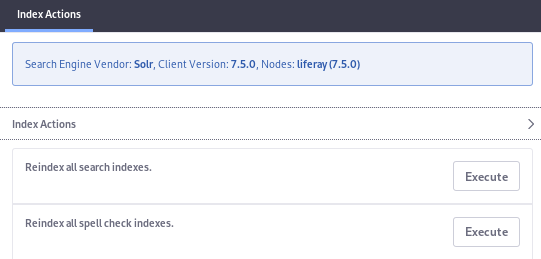
\includegraphics{./images/solr-reindex.png}
\caption{Once the Solr connector is installed, you can re-index your
Liferay DXP data against your Solr server.}
\end{figure}

In production deployments, specify your edits to the Solr connector's
default configurations using a configuration file deployed to the
\texttt{Liferay\_Home/osgi/configs} folder. Name the file

\begin{verbatim}
com.liferay.portal.search.solr7.configuration.SolrConfiguration.config
\end{verbatim}

During testing and development, use the Solr 7 System Settings entry
Control Panel → Configuration → System Settings for editing the default
configurations.

\begin{figure}
\centering
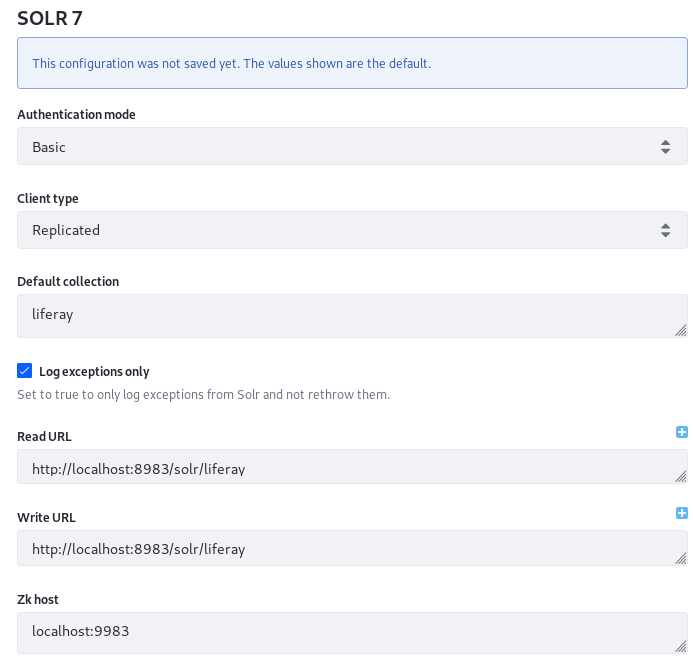
\includegraphics{./images/solr-system-settings.png}
\caption{You can configure Solr from Liferay DXP's System Settings
application. This is most useful during development and testing.}
\end{figure}

The next article covers clustering Solr with SolrCloud.

\section{Installing Solr: High Availability with
SolrCloud}\label{installing-solr-high-availability-with-solrcloud}

\noindent\hrulefill

\textbf{Note:} To install Solr 8, see the Solr installation guide on
\href{https://learn.liferay.com/dxp/latest/en/using-search/installing-and-upgrading-a-search-engine/solr/installing-solr.html}{Liferay
Learn}

\noindent\hrulefill

Use SolrCloud if you need a cluster of Solr servers. Note that to use
SolrCloud in production, you should set up an
\href{https://cwiki.apache.org/confluence/display/solr/Setting+Up+an+External+ZooKeeper+Ensemble}{external
ZooKeeper ensemble}. \href{http://zookeeper.apache.org/}{ZooKeeper} is a
centralized coordination service for managing distributed systems like
your SolrCloud cluster.

The steps included here should be considered the bare minimum of what
must be done to configure SolrCloud with Liferay DXP. For example, these
instructions cover configuring SolrCloud on a single machine, whereas a
production environment would feature multiple physical or virtual
machines. These instructions also assume you've followed the earlier
section on \emph{Installing and Configuring Solr 7}. Refer to the
\href{https://cwiki.apache.org/confluence/display/solr/SolrCloud}{SolrCloud
guide for more information}.

\begin{enumerate}
\def\labelenumi{\arabic{enumi}.}
\item
  Stop the Solr server if it's running.
\item
  Navigate to the \texttt{Solr\_Home/configsets} folder and create a
  folder called

\begin{verbatim}
 liferay_configs
\end{verbatim}
\item
  Copy the \texttt{conf} folder from \texttt{Solr\_Home/liferay} to the
  \texttt{liferay\_configs} folder you just created.

  The \texttt{configset/liferay\_configs} folder contains the SolrCloud
  Liferay DXP collection configuration and is uploaded to ZooKeeper. By
  copying the \texttt{conf} folder from the \texttt{liferay} server
  configured earlier, you're using the \texttt{schema.xml} and
  \texttt{solrconfig.xml} files provided with the Liferay Solr Adapter.
\item
  Next launch an interactive SolrCloud session to configure your
  SolrCloud cluster. Use this command:

\begin{verbatim}
 ./bin/solr -e cloud
\end{verbatim}
\item
  Complete the setup wizard. These steps demonstrate creating a two-node
  cluster:

  \begin{itemize}
  \item
    Enter \texttt{2} for the number of nodes.
  \item
    Specify ports \texttt{8983} and \texttt{7574} (the defaults). Both
    nodes are started with the start commands printed in the log:

\begin{verbatim}
     Starting up Solr on port 8983 using command:
     "bin/solr" start -cloud -p 8983 -s "example/cloud/node1/solr"
\end{verbatim}
  \item
    Name the collection \emph{liferay}.
  \item
    Split the collection into two shards.
  \item
    Specify two replicas per shard.
  \item
    When prompted to choose a configuration, enter
    \emph{liferay\_configs}. You should see a log message that concludes
    like this when the cluster has been started:

\begin{verbatim}
     SolrCloud example running, please visit http://localhost:8983/solr
\end{verbatim}
  \end{itemize}
\end{enumerate}

Now you have a new collection called \emph{liferay} in your local
SolrCloud cluster. Verify its status by running the \emph{status}
command:

\begin{verbatim}
./bin/solr status
\end{verbatim}

You'll see log output like this:

\begin{verbatim}
Found 2 Solr nodes: 

Solr process 16989 running on port 8983
INFO  - 2018-08-06 13:54:17.665; org.apache.solr.util.configuration.SSLCredentialProviderFactory; Processing SSL Credential Provider chain: env;sysprop
{
  "solr_home":"/home/russell/liferay-bundles/solr-7-dxp/solr-7.4.0/example/cloud/node1/solr",
  "version":"7.4.0 9060ac689c270b02143f375de0348b7f626adebc - jpountz - 2018-06-18 16:55:13",
  "startTime":"2018-08-06T17:52:01.519Z",
  "uptime":"0 days, 0 hours, 2 minutes, 16 seconds",
  "memory":"68.5 MB (%14) of 490.7 MB",
  "cloud":{
    "ZooKeeper":"localhost:9983",
    "liveNodes":"2",
    "collections":"1"}}


Solr process 17127 running on port 7574
INFO  - 2018-08-06 13:54:18.507; org.apache.solr.util.configuration.SSLCredentialProviderFactory; Processing SSL Credential Provider chain: env;sysprop
{
  "solr_home":"/home/russell/liferay-bundles/solr-7-dxp/solr-7.4.0/example/cloud/node2/solr",
  "version":"7.4.0 9060ac689c270b02143f375de0348b7f626adebc - jpountz - 2018-06-18 16:55:13",
  "startTime":"2018-08-06T17:52:11.987Z",
  "uptime":"0 days, 0 hours, 2 minutes, 6 seconds",
  "memory":"56.4 MB (%11.5) of 490.7 MB",
  "cloud":{
    "ZooKeeper":"localhost:9983",
    "liveNodes":"2",
    "collections":"1"}}
\end{verbatim}

To stop Solr while running in SolrCloud mode, use the \emph{stop}
command, like this:

\begin{verbatim}
bin/solr stop -all
\end{verbatim}

\subsection{Configure the Solr Adapter for
SolrCloud}\label{configure-the-solr-adapter-for-solrcloud}

There's only one thing left to do: specify the client type as
\emph{CLOUD} in Liferay's Solr connector.

\begin{enumerate}
\def\labelenumi{\arabic{enumi}.}
\item
  From System Settings or your OSGi configuration file, set the
  \emph{Client Type} to \emph{CLOUD}.

\begin{verbatim}
 clientType="CLOUD"
\end{verbatim}
\item
  Start Liferay DXP if it's not running already.
\end{enumerate}

\begin{figure}
\centering
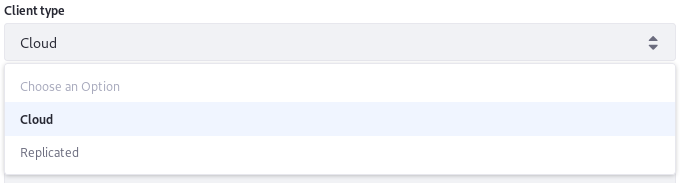
\includegraphics{./images/solr-client-type.png}
\caption{From the Solr 7 System Settings entry, set the \emph{Client
Type} to \emph{Cloud}.}
\end{figure}

WC template \textbar{} Template is deleted \textbar{} The feed can exist
without the template. It is not validated. \textbar{} Renderer template
is deleted \textbar{} The feed can exist without the template. It is not
validated. Page \textbar{} Page's friendly URL is modified \textbar{}
The link to the page still works. \textbar{} Portlet is removed from
page \textbar{} The feed can live without a portlet ID; the portlet is
removed upon publication. Display page \textbar{} WC article with
display pages is configured \textbar{} The page, Asset Publisher
portlet, and content are published. \textbar{} Display page is deleted
\textbar{} The page and its content are deleted. \textbar{} WC article
is deleted \textbar{} The article deletion is published; the display
page is not affected. \textbar{} WC article with a display page is added
but the page was not published earlier and it's not included in the
publication \textbar{} The page reference is validated and the
publication fails when the page is not there. A message displays
explaining this to the user.

\noindent\hrulefill

\subsection{Wiki}\label{wiki}

The following table describes how entities that are attached/related to
Wikis are handled by the Staging framework.

\noindent\hrulefill

\begin{longtable}[]{@{}
  >{\raggedright\arraybackslash}p{(\columnwidth - 4\tabcolsep) * \real{0.2414}}
  >{\raggedright\arraybackslash}p{(\columnwidth - 4\tabcolsep) * \real{0.2586}}
  >{\raggedright\arraybackslash}p{(\columnwidth - 4\tabcolsep) * \real{0.5000}}@{}}
\toprule\noalign{}
\begin{minipage}[b]{\linewidth}\raggedright
Related entity
\end{minipage} & \begin{minipage}[b]{\linewidth}\raggedright
Action performed
\end{minipage} & \begin{minipage}[b]{\linewidth}\raggedright
How does Staging handle this?
\end{minipage} \\
\midrule\noalign{}
\endhead
\bottomrule\noalign{}
\endlastfoot
Attachment link & Add a link to an attachment of the same page to a wiki
page & The attachment is published and the link in the wiki points to
the new attachment. \\
Add a link to another wiki page of the same node to a wiki page & The
wiki page is published, but the link is not. & \\
Parent wiki page & Add a wiki page and a child of that page & Both pages
are published. \\
Parent page is deleted & The parent page and all its children are
deleted. & \\
Child page is deleted & The child page deletion is published. & \\
Parent page is updated & The updated page is published. & \\
Child page is updated & The updated page is published. & \\
Wiki redirect page & Page is moved to a new title & The pages are
updated and published; the redirect works on the live site. \\
Intermediate page is deleted & The page deletion is published; the new
page is not affected. & \\
Target page is deleted & Both the intermediate and new page are deleted
and those deletions are published. & \\
Site link in content & Add a link to a Liferay site page to wiki & The
new wiki content and the site page referenced in the link are
published. \\
Wiki node & New node is added & The node is published. \\
Node is updated & The node is published. & \\
Set of pages is imported into existing node & The pages are published.
& \\
Node is deleted & The node and all its dependent pages are deleted and
those deletions are published. & \\
Wiki page & Page with no child/parent relationships is copied & The new
page is published. \\
Page containing a child is moved, changing its title and parent & The
page is published. After publication, the page is located under a new
parent and has a new name. The child points to the new page. & \\
Page with no child/parent relationships is deleted & The page deletion
is published. & \\
Attachment is removed from page & The page is published. The attachment
is removed from the page on the live site. & \\
Category is removed from page & The page is published. The category is
removed from the page on the live site. & \\
Page format is modified & The page is published. & \\
Image (not yet published) is added to page's content & The page and its
image are published. & \\
\end{longtable}
